\setchapterpreamble[u]{\margintoc}
\chapter{Simulation of LiDAR sensors}
\labch{lidar_simulation}
\label{sec:lidar_simulation}

\section*{About this chapter}

This chapter presents a synthetic \acrshort{gpu}-based \acrshort{lidar} scanner. It is parameterized to emulate a large number of sensor models, ranging from airborne to terrestrial scanning. The approach is massively parallelized in the \acrshort{gpu} to solve millions of intersections with a reduced response time, even simulating multiple returns for scenarios aimed at modelling forestry. This work is mainly intended for the rapid generation of large \acrshort{lidar} datasets for Deep Learning. The conducted experiments show that the proposed approach outperforms a sequential approach, and the capabilities for constructing large datasets were proven to enhance previous work. 

\begin{marginfigure}[6cm]
    \centering
    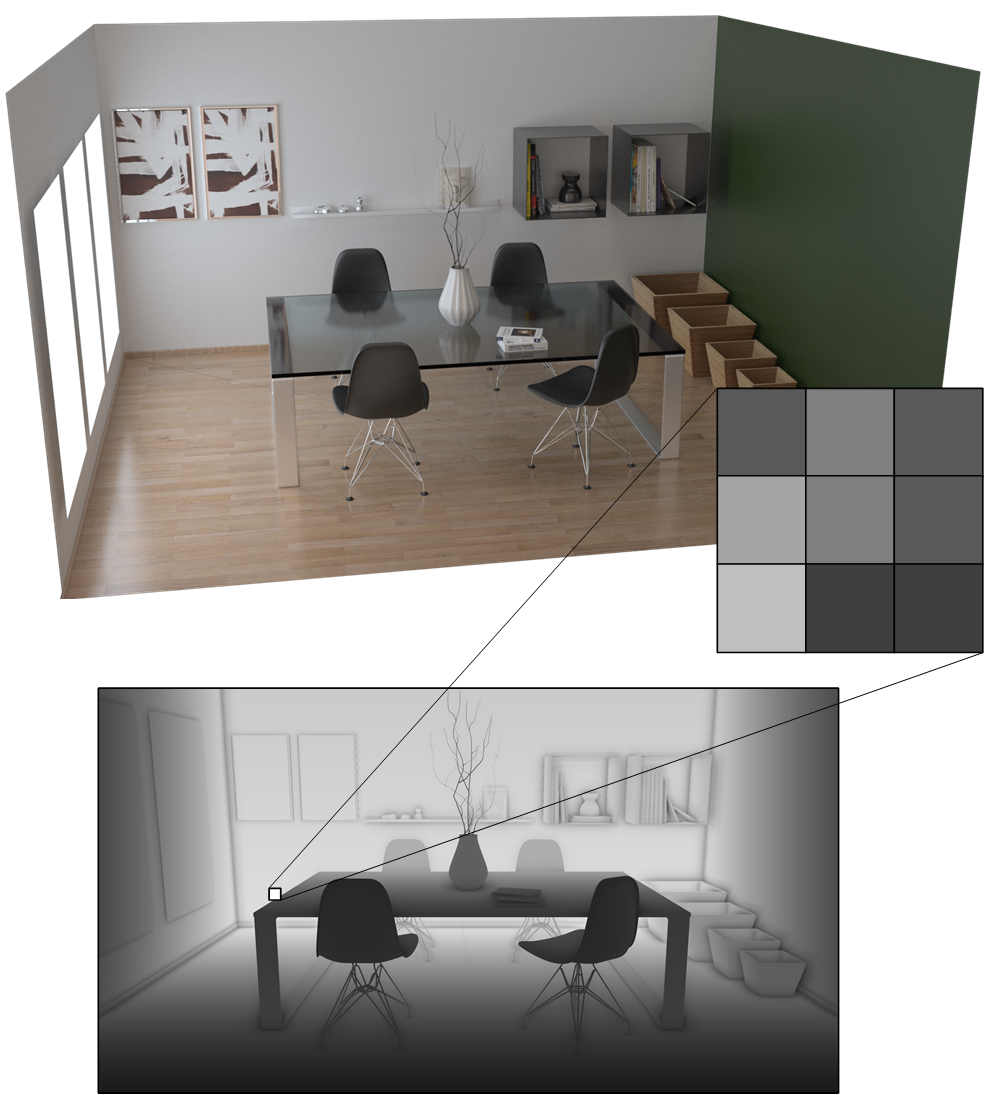
\includegraphics[width=\linewidth]{figs/lidar_simulation/depth_buffer.png}
	\caption{Depth buffer of a 3D scene, as proposed in previous \acrshort{lidar} simulations. }
	\label{fig:depth_buffer_lidar}
\end{marginfigure}
Another key factor is the use of procedural 3D environments; scenes modelled by professionals can be utilized for generating a few datasets using several viewpoints or paths, whereas those governed by generation rules help to construct a large number of datasets depicting different environments. Besides \acrshort{tls}, which is by far the most studied kind of \acrshort{lidar} sensor, this chapter is also intended for describing how to simulate aerial surveys comprising sensor errors and surface properties. In comparison with previous work, collisions are solved using state-of-the-art ray-tracing data structures, instead of \textit{z}-buffers with a limited resolution (Figure \ref{fig:depth_buffer_lidar}). Consequently, this piece of software is able to construct high-quality point clouds with low latency. 

% Nevertheless, working in the image space is sometimes required; for instance, Deep Learning models are easier to operate in images than over 3D point clouds without losing precision on them (e.g., by voxelizing).

In comparison with previous work, the main contributions of this chapter are the generation of large labelled \acrshort{lidar} datasets from procedural scenarios. These are obtained in a reduced response time following a physically-based interaction, while a sequential approach requires several minutes, even hours, for solving complete scans of the inspected scenario. The overall workflow is depicted in Figure \ref{fig:lidar_overview}. 

\section{On the generation of LiDAR datasets}

\acrshort{lidar} technology has rapidly evolved in the last two decades and therefore, it has received great attention from industrial and academic environments. This sensor enables acquiring information about a surface, object or phenomenon without physical contact. There is a wide variety of \acrshort{lidar} variants according to the sensor capabilities, the platform on which they are operated (\acrshort{tls}, \acrshort{als}, \acrshort{mms}, \acrshort{bmmls}, etc.), manufacturers and models. Unfortunately, it is not easy to get a sufficient amount of ground truth data due to time constraints and available resources. In contrast to real \acrshort{lidar} sensors, \acrshort{lidar} simulation enables the generation of classified data at a significantly lower cost. The cost of \acrshort{lidar} technology is prohibitive, and collecting large real-world datasets is time-consuming, both in the acquisition and labelling (if required). 

On the other hand, simulated \acrshort{lidar} data can be enriched with any kind of information. For instance, semantic tags can be accurately determined since the models in the input scenarios are named accordingly. The \acrshort{lod} of augmented data, including semantic tags, can be constrained by the \acrshort{lod} of input environments as well as by the requirements of decision-making and classification algorithms that will use these synthetic datasets. Also, simulations can go further and integrate errors and limitations of \acrshort{lidar}, either systematic or random, to provide more realistic data. Nevertheless, simulating the physical interaction of \acrshort{lidar} sensors with real-world surfaces is a non-trivial task that demands computationally efficient algorithms. 

\begin{figure*}
    \centering
    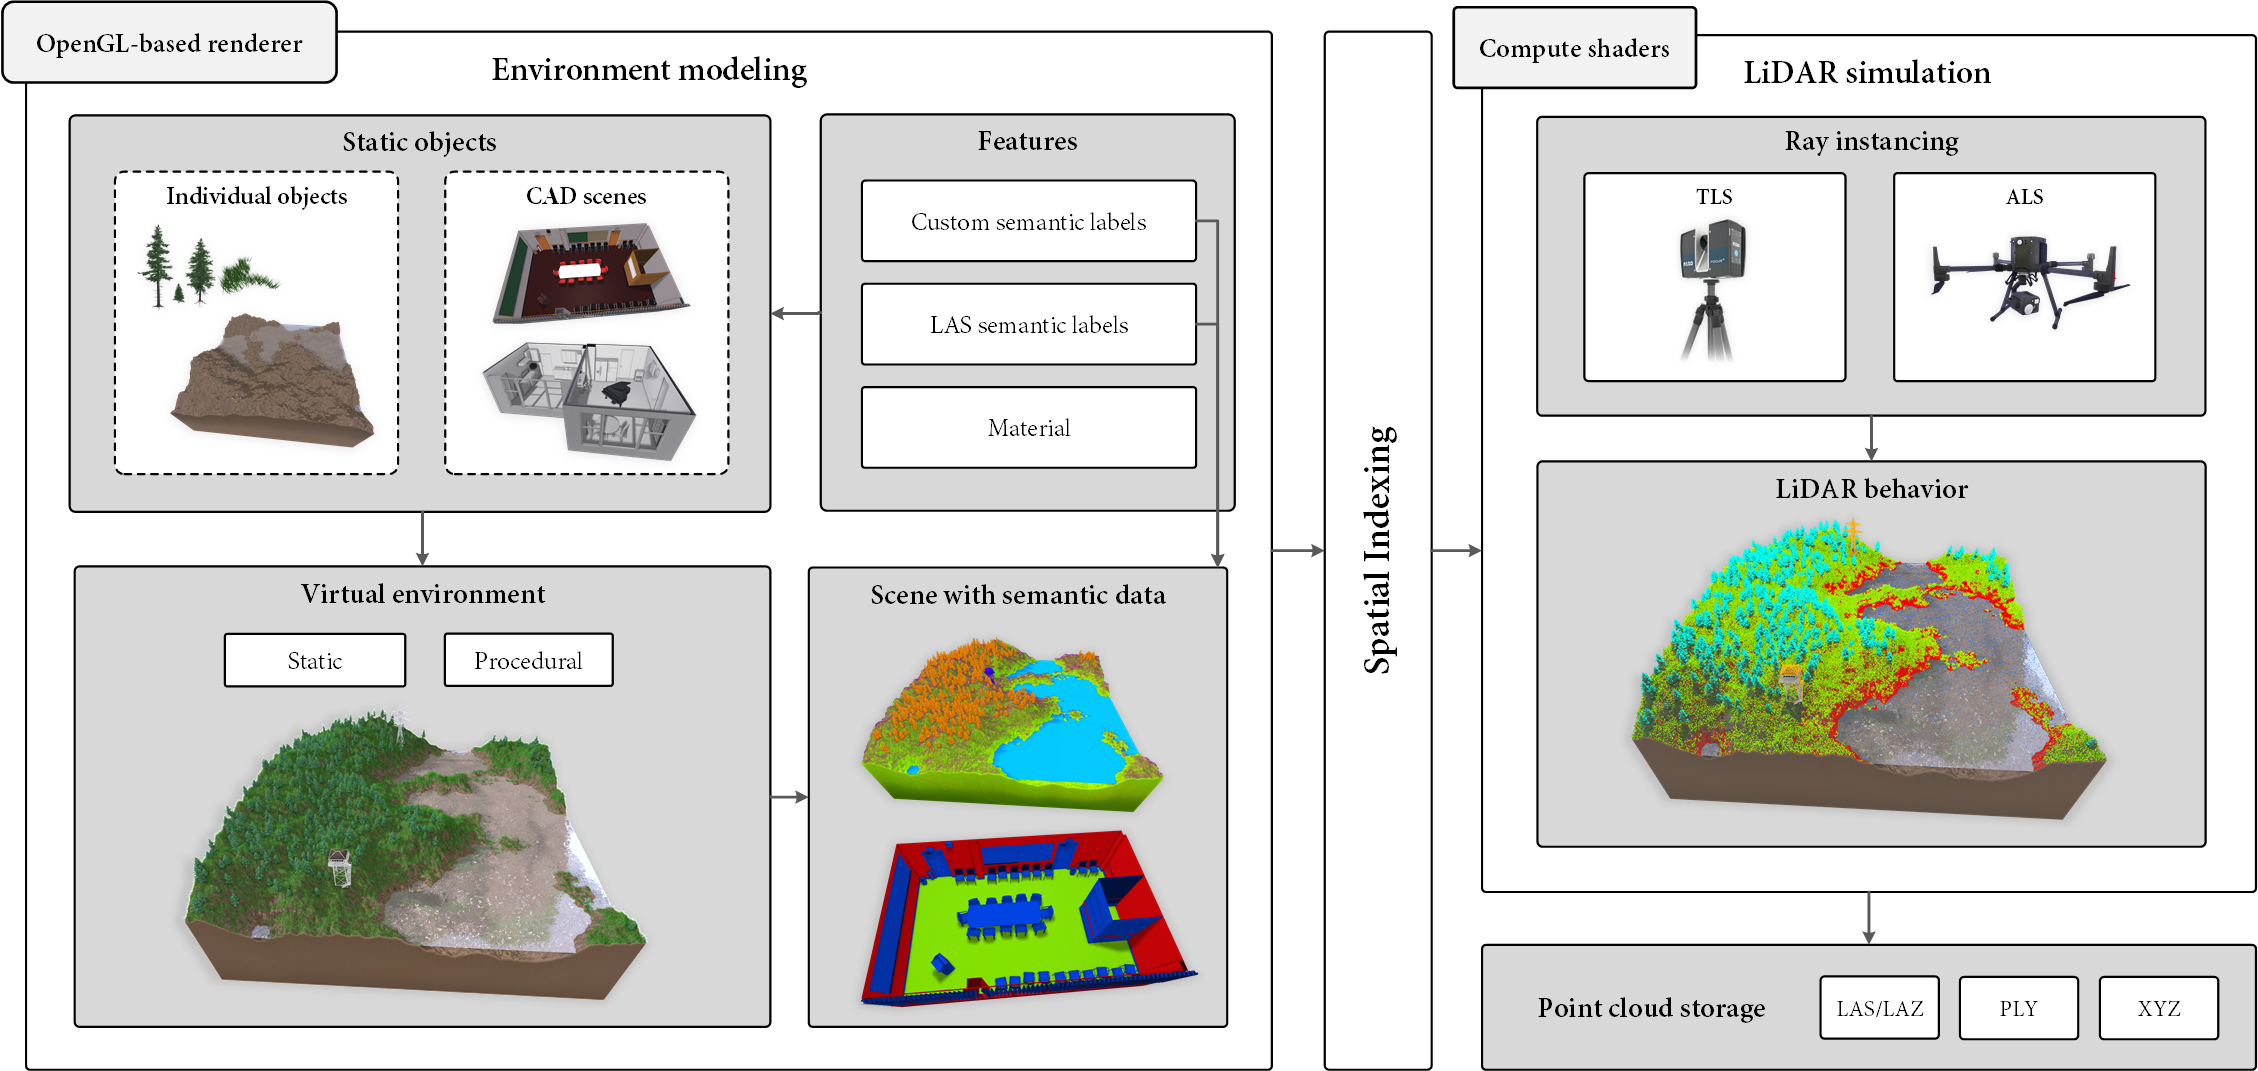
\includegraphics[width=\linewidth]{figs/lidar_simulation/overview.png}
	\caption{Overview of a \acrshort{lidar} simulator operating over 3D virtual scenes, either procedural or static, which are previously indexed to speed up spatial queries. }
	\label{fig:lidar_overview}
\end{figure*}

\section{Modelling of synthetic environments}

Synthetic scenarios must be similar to real-world environments since the scanning results are aimed at feeding \acrshort{dl} algorithms. Furthermore, procedural scenarios are preferred over those modelled by professionals in the generation of large datasets, since the former lead to a greater variety. Following this approach, scenarios can be generated using rules that determine how will be distributed a collection of 3D models. In contrast to static scenarios, the labelling of procedural environments is more efficient as it is only performed once. Although there exists third-party software for the generation of procedural environments, such as SpeedTree\textregistered, a custom tool was implemented to meet our specific requirements and enable the labelling of every model instance. 

\newpage
\subsection{Forestry environments}

\begin{marginfigure}[.cm]
    \centering
    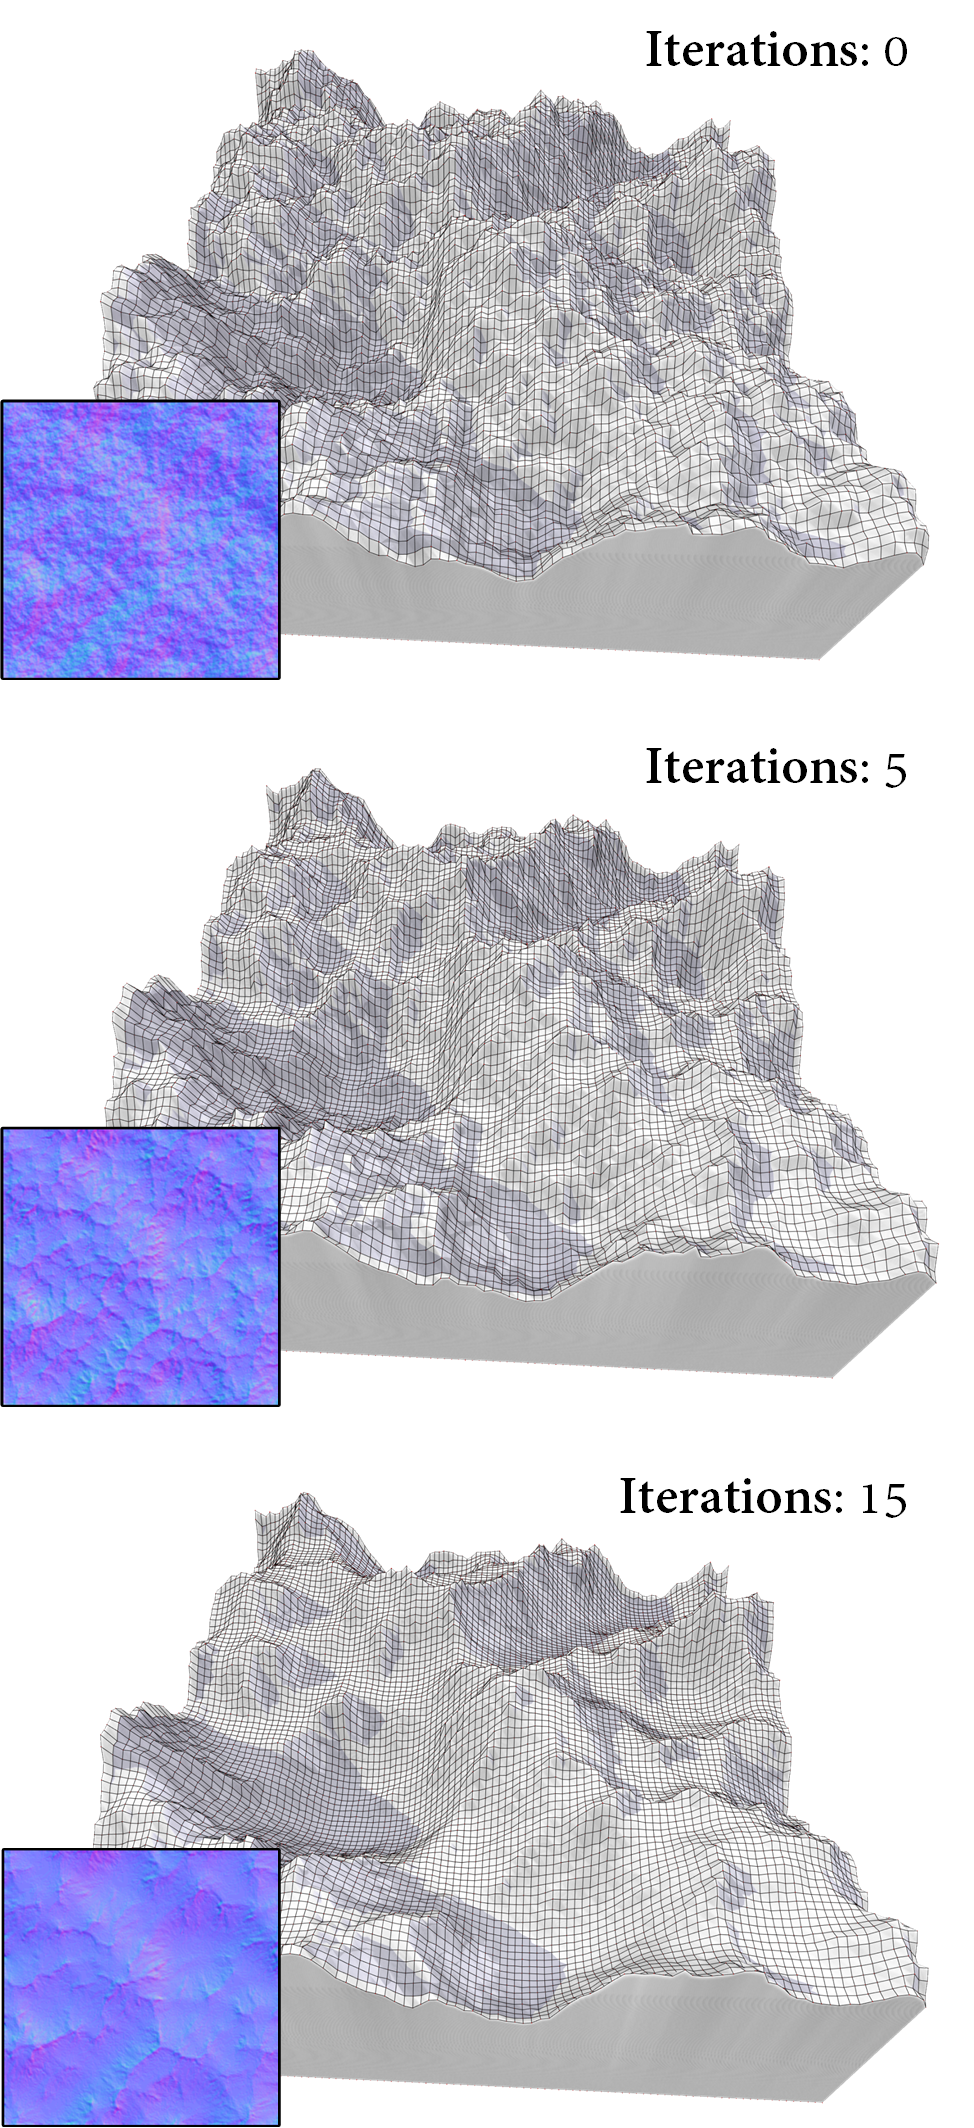
\includegraphics[width=\linewidth]{figs/lidar_simulation/erosion.png}
	\caption{Hydraulic erosion of 200k particles over a heightfield modelled with 2D Perlin noise. }
	\label{fig:hydraulic_erosion}
\end{marginfigure}
The procedural generation of forestry scenarios has been previously approached with ecosystems \cite{cordonnier_authoring_2017, fischer_autobiomes_2020, makowski_synthetic_2019} that achieve a high level of realism. However, this work intended to provide a simple tool for the procedural generation of natural scenarios. To this end, the procedure depicted in Figure \ref{fig:procedural_workflow} can be configured using a text file or a node editor in the Graphical User Interface (\acrshort{gui}).

\begin{figure*}
    \centering
    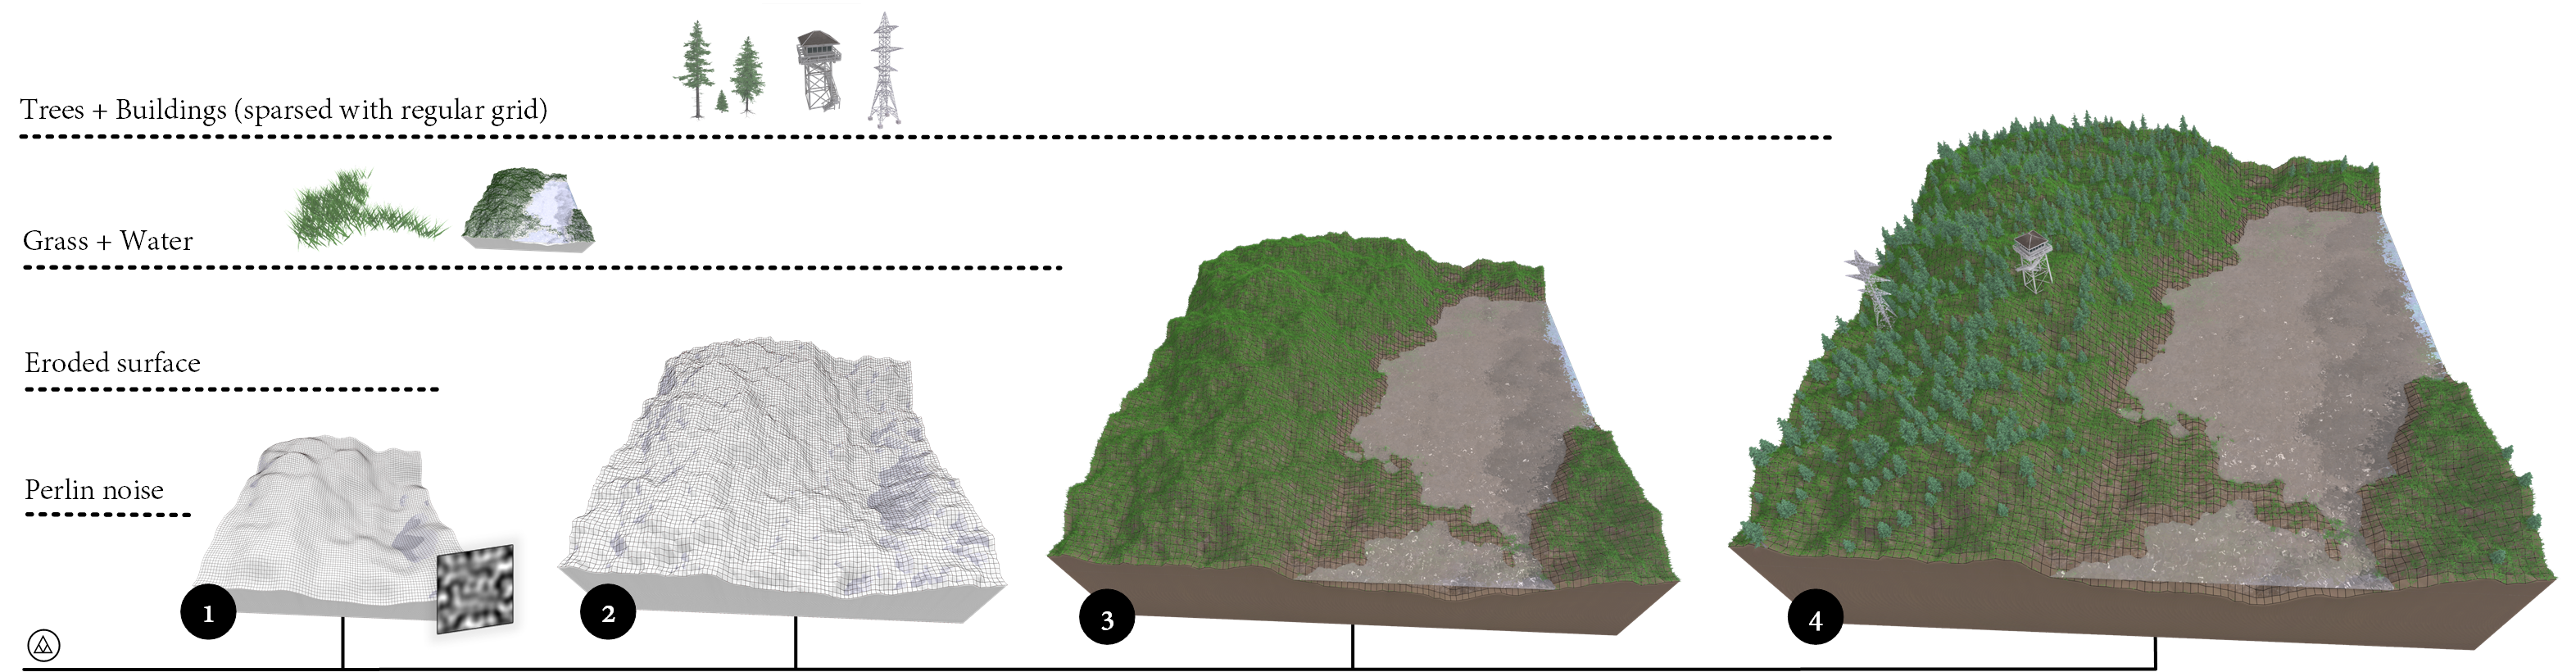
\includegraphics[width=\linewidth]{figs/lidar_simulation/procedural_workflow.png}
	\caption{Workflow regarding the procedural modelling of a forestry area with water, low-vegetation, high-vegetation and buildings. First, the soil is eroded using hydraulic processes, and then, water and low vegetation are procedurally generated. Finally, trees and buildings are generated so that collisions among them are avoided. }
	\label{fig:procedural_workflow}
\end{figure*}

The soil was modelled using a Perlin noise function, followed by hydraulic erosion over the heightfield representation of the terrain. The erosion algorithm was enhanced using the \acrshort{gpu} to model each particle with a different thread. Accordingly, the particles move according to a weighted aggregation of slopes from their surroundings, until a move of length zero or a limit of iterations ($\rho_{\textit{iterations}}$) are reached. During these moves, particles deposit sediment whether the carried material exceeds their capacity; otherwise, the heightfield is eroded. The erosion is applied as a convolution with a configurable radius, whose weights, $w_i$, represent the distance to the kernel centre. Regardless of the particle location, the convolution has always the same weights and thus can be computed once and stored. Figure \ref{fig:hydraulic_erosion} shows several stages of this hydraulic erosion for 200k particles. The surface got smoother when the erosion run for a larger number of iterations. Hence, a limited number of iterations helps to balance realism and latency. 

On the other hand, water is modelled as planar surfaces placed at valleys. The procedure is to locate local minima defined as points whose elevation is lower than surrounding pixels. Then, local minima points are flooded until the height $h_{\textit{flood}}$ is achieved to compute which cells are part of a valley. $h_{\textit{flood}}$ is computed as shown in Equation \ref{eq:water_height} using a reference height, $h_{\textit{water}}$, and a random value in $[-h_{\sigma}, h_{\sigma}]$, both obtained from the scene configuration. The set of collected valleys is sorted according to the covered area to retrieve only the top-$n$ instances. 
\begin{equation}
    \label{eq:water_height}
    h_{\textit{flood}} = h_{\textit{water}} + f_{\textit{random}}h_{\sigma}
\end{equation}
where $f_{\textit{random}} \in [-1, 1]$.

\begin{marginfigure}[1.0cm]
    \centering
    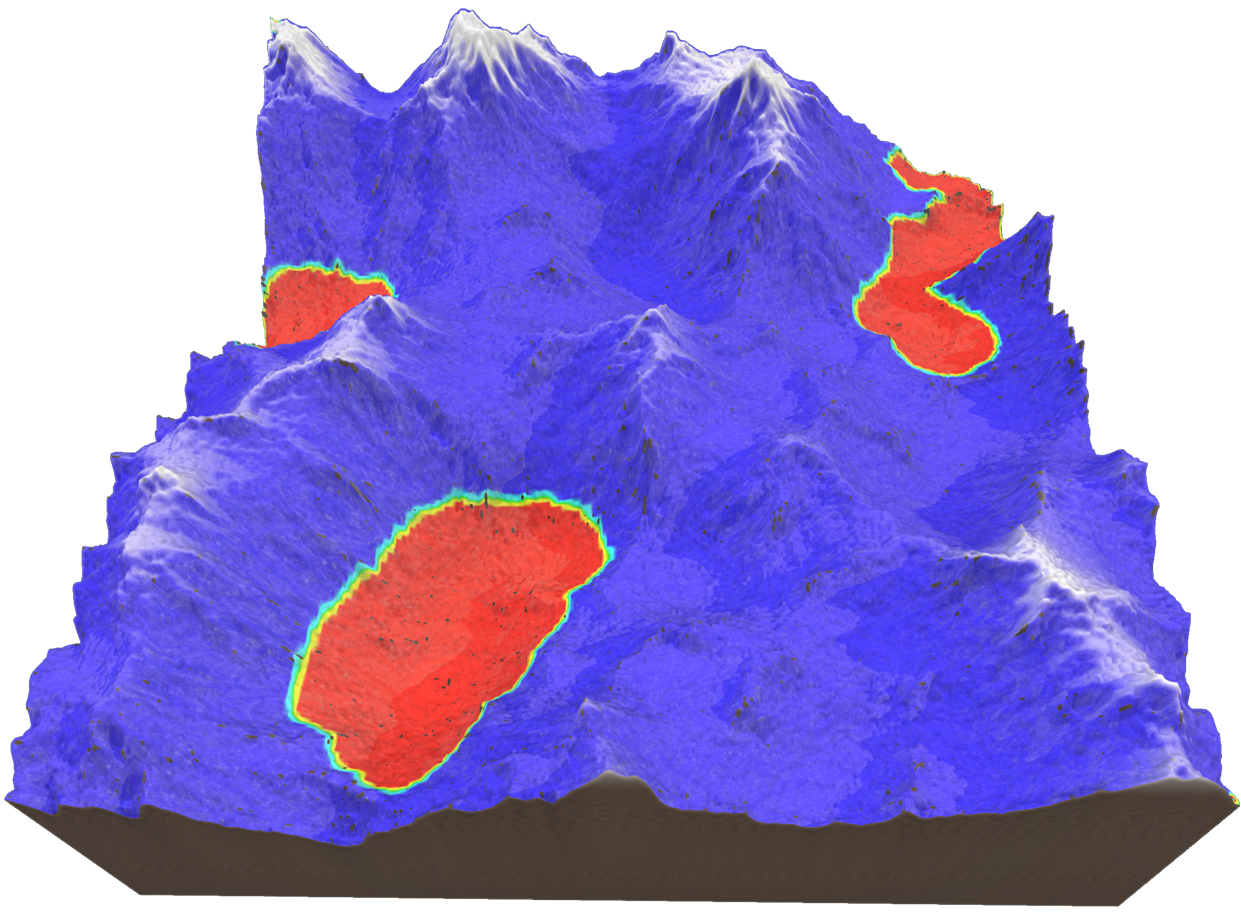
\includegraphics[width=\linewidth]{figs/lidar_simulation/valley_finds.png}
	\caption{Valleys detected on an eroded terrain. }
	\label{fig:terrain_valleys}
\end{marginfigure}
Low vegetation is represented with a large number of low-poly instances that enable the modelling of highly detailed scenes while keeping a good rendering performance. Still, \acrshort{opengl}'s instance rendering is required for providing a high value of \acrshort{fps}. Otherwise, geometry shaders could be used; however, the \acrshort{lidar} simulation requires explicitly declaring the vegetation geometry in a \acrshort{ssbo} for the spatial indexing. The distribution was computed using seeds from a random uniform distribution, with the slope and height being key factors to determine whether they are instanced or not. Thus, the instancing probability is defined as shown in Equation \ref{eq:vegetation_instancing_prob}. The probability map is compiled in a texture that aggregates the height and normal map computed in previous stages. According to Equation \ref{eq:vegetation_instancing_prob}, points that present steeper slopes and lower altitudes have a lower instancing probability.
\begin{gather}
    \label{eq:vegetation_instancing_prob}
    p_{i, j} = 1 - w_{\textit{height}} \cdot H(h, h_{\textit{min}}, h_{\textit{max}}) - w_{\textit{slope}} \cdot (1 - \hat{n} \cdot \left[0, 1, 0\right]^\intercal)
\end{gather}
where $H(h, h_{\textit{min}}, h_{\textit{max}})$ is an Hermite interpolation function in $[h_{\textit{min}}, h_{\textit{max}}]$, and $\hat{n}$ is the normal vector at $(i, j)$, given that $i \in [0, \textit{width}[$ and $j \in [0, \textit{height}[$, with ($\textit{width}, \textit{height}$) being the size of the eroded heightfield.

\begin{figure*}[hbt]
    \centering
    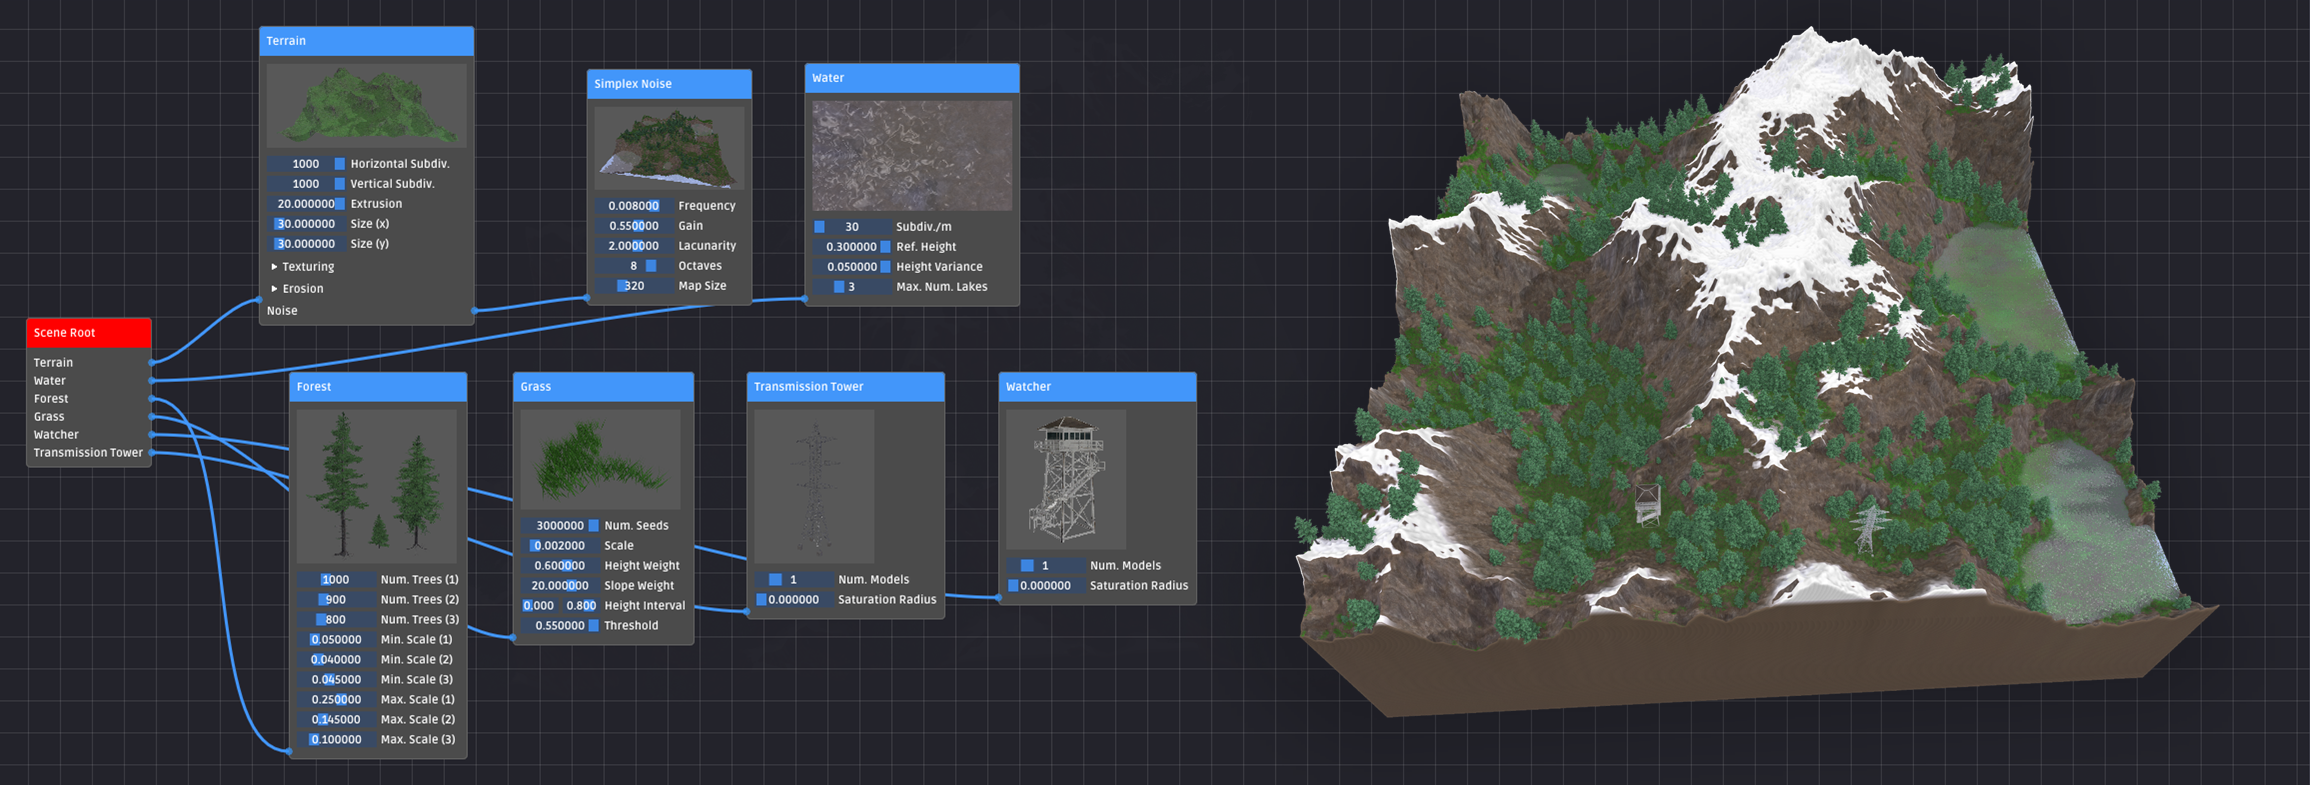
\includegraphics[width=\linewidth]{figs/lidar_simulation/node_editor.png}
	\caption{Configuration of the node editor for constructing an environment such as the one depicted on the right side.  }
	\label{fig:node_editor}
\end{figure*}

In contrast to low vegetation, the instancing of trees also takes into account previously instanced geometry to avoid intersecting it. Instead of checking collisions among triangle meshes, it was simplified using a 2D regular grid that narrows the problem to check whether a cell is already occupied or saturated. According to this, the grid cells are saturated with a factor of $f_{\textit{saturation}}$ within a radius $r$ when a new object is instanced. On the other hand, a grid cell is considered to be saturated whether its occupation is over a threshold, $h_{\textit{saturation}}$. Therefore, the density of vegetation is coarsely controlled with the grid subdivision and $h_{\textit{saturation}}$. Whenever a grid cell must be occupied by a single model, it can be saturated with a value of $\infty$. 

\subsection{Urban environments}

Urban scenarios are partly modelled as procedural environments (see Figure \ref{fig:procedural_urban}). The baseline is a large city and residential scenario modelled by professionals, whereas pedestrians and vehicles are procedurally instanced. To this end, candidate seeds are sparsed over sidewalks and road models and instanced whether the linked random value is below a threshold. The instancing frequency as well as the varying scale of each model can be configured. 

\begin{marginfigure}[.2cm]
    \centering
    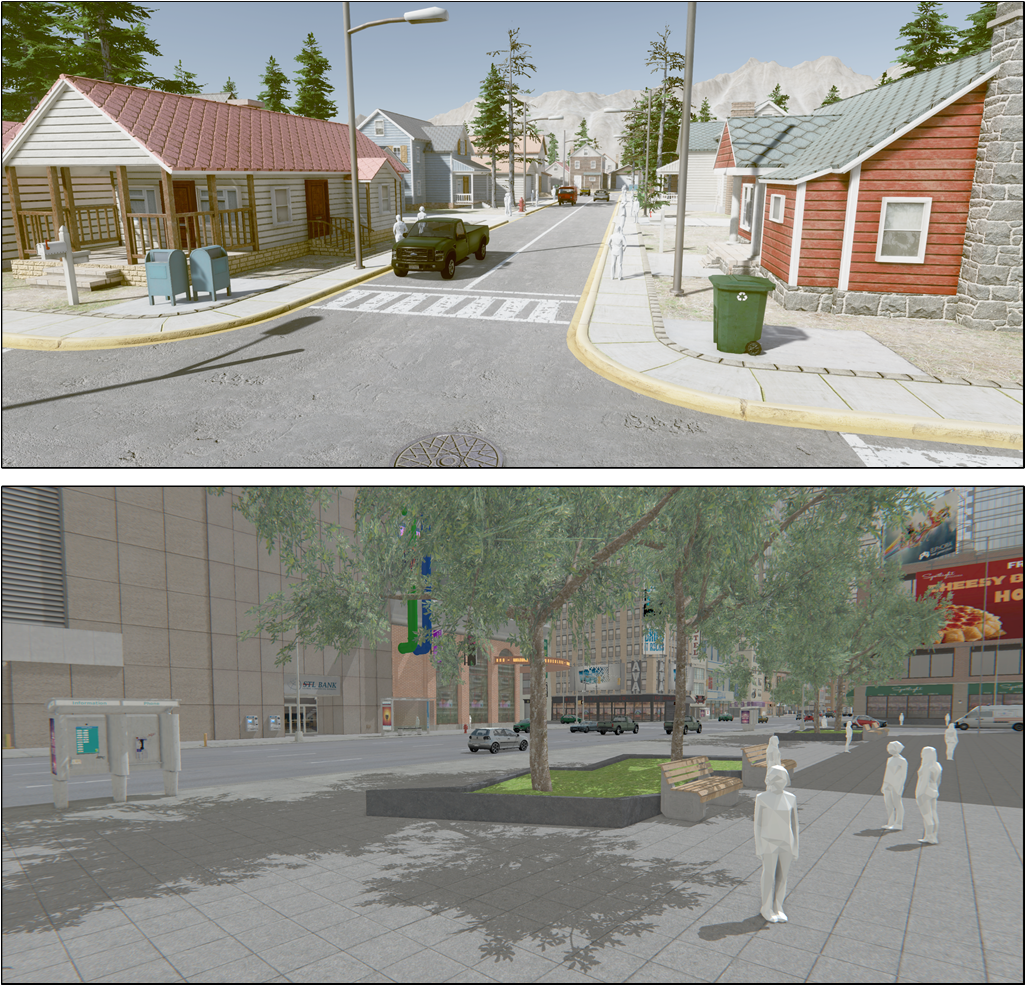
\includegraphics[width=\linewidth]{figs/lidar_simulation/procedural_urban.png}
	\caption{Procedural urban environment based on a) a residential area and b) a metropolis. }
	\label{fig:procedural_urban}
\end{marginfigure}
\begin{marginfigure} [8.cm]
	\centering
	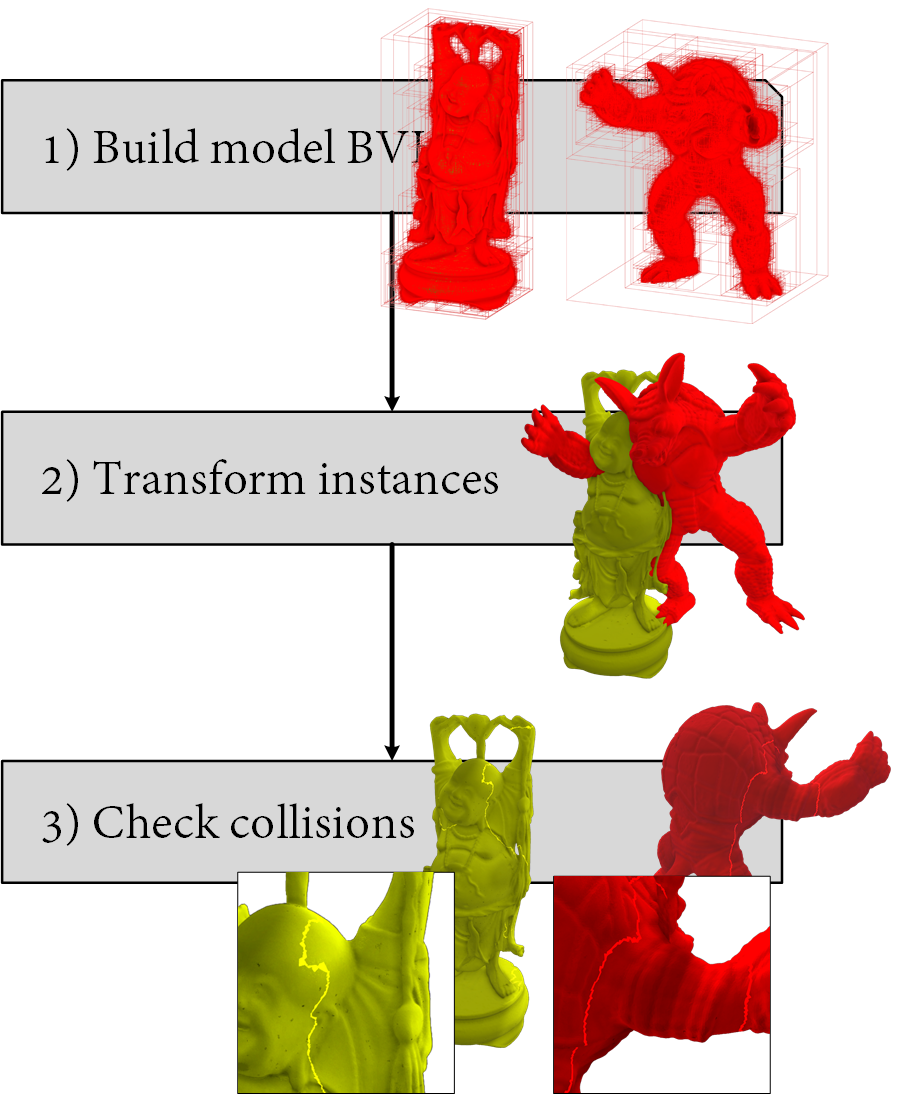
\includegraphics[width=\linewidth]{figs/lidar_simulation/mesh_collision.png}
	\caption{Detection of collisions between two triangle meshes. }
	\label{fig:triangle_mesh_collision}
\end{marginfigure}
Firstly, roads are split into rails according to their width, and then, vehicles are rotated using the road rotation matrix. The location is computed by selecting a random road and rail, as well as a random translation within it. On the other hand, the \textit{y} coordinate is computed as the collision of a ray emitted towards the road with $\textit{nadir}$ direction, plus half the height of the vehicle's bounding box. The main concern during the instancing of vehicles is to avoid inter-collisions. Hence, these can be detected by building the \acrshort{bvh} of each different model and rapidly determining if there are collided polygons. However, doing this for every instance is very time-consuming; instead, \acrshort{bvh}s are built for every model in the database, and they can be changed according to the instance's transformation matrix (Figure \ref{fig:triangle_mesh_collision}). Still, transforming every vertex is time-consuming, and thus, collisions between triangles can be identified by casting rays with the shape of the edges of every source model's triangle. With this approach, three rays are cast for every triangle, with its coordinates being transformed as shown in Equation \ref{eq:mesh_collision_ray}. Rather than comparing the new instance with the rest, it is narrowed using a 2D regular grid whose subdivision length corresponds to the maximum \textit{xz} length from any collected vehicle. Similarly, the source model from which rays are emitted is selected as the one with the lower number of polygons.
\begin{gather}
    \label{eq:mesh_collision_ray}
    \begin{aligned}
        r_{o} &= \inv{C_{T}} \cdot C_{S} \cdot v_{\textit{source}}\\
        r_{t} &= \inv{C_{T}} \cdot C_{S} \cdot v_{\textit{target}}\\
        r_{d} &= \widehat{r_{t} - r_{o}}
    \end{aligned}
\end{gather}
where $r_{o}$, $r_{t}$ and $r_{d}$ are the ray's source, target and direction, and the vertices $v_{\textit{source}}$, $v_{\textit{target}}$ are part of a triangle edge. Composite matrices ($C$) with $T$ subscript correspond to the target model, whereas $S$ refers to the source instance, i.e., the model with a lower number of polygons.

On the other hand, translation and rotation vectors are significantly more randomized for pedestrian instancing. Pedestrian models are randomly selected, whereas their location and rotation in the $y$-axis are described using three random values ($t_x$, $t_z$, $r_y$). As proposed before, the $y$ coordinate can be obtained by casting a ray with $\textit{nadir}$ direction. The detection of inter-collisions is addressed as explained, though pedestrians may also collide with buildings. Thus, it requires building the \acrshort{bvh} of non-populated urban objects. Finally, procedural trees are also generated in some areas, and they can be upscaled and downscaled within a user-defined interval.

\section{Spatial indexing}

The objective of the synthetic \acrshort{lidar} that will be following proposed is to estimate returns with high precision. To this end, these will be computed with ray-casting in 3D, rather than solving it in the image space. However, highly detailed scenarios are composed of several millions of triangles and \acrshort{lidar} simulations also comprise millions of rays. Despite ray-triangle intersections being efficiently solved in the \acrshort{gpu}, the main concern is the spatial traversal since it is considerably more time-consuming. Thus, this is a well-known time bottleneck even for optimized proposals. 

\begin{marginfigure}[.cm]
    \centering
    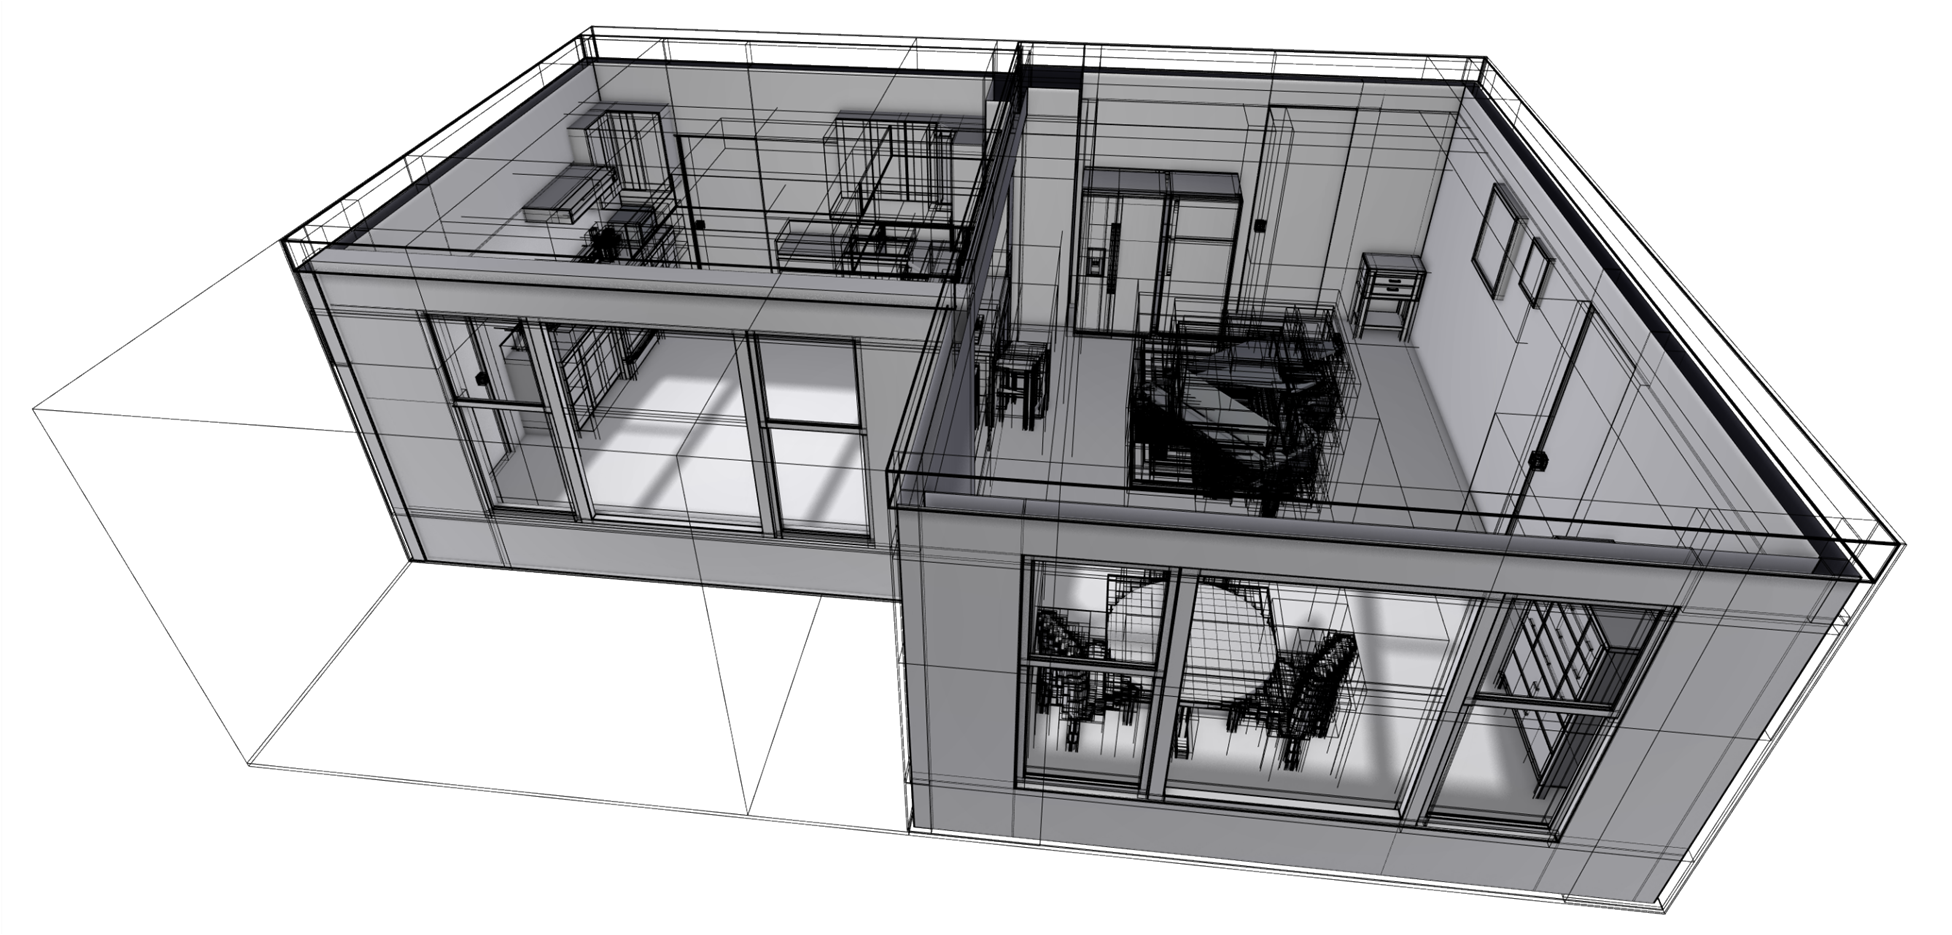
\includegraphics[width=\linewidth]{figs/lidar_simulation/bvh_rendering.png}
	\caption{Rendering of the \acrshort{bvh} indexing of the very same scene in \ref{fig:kitchen_classification}. It was constructed using a buffer radius, $r$, of size 100.}
	\label{fig:lidar_bvh_rendering}
\end{marginfigure}
Either static or procedural, scenarios are indexed using a \acrshort{bvh} which can be rapidly traversed for millions of rays. The indexing was performed as proposed by Meister and Bittner \cite{meister_parallel_2018} in the \acrshort{gpu}. Hence, it is efficiently generated and after this, the \acrshort{bvh} is stored in the \acrshort{gpu}'s memory to solve the subsequent scans, thus avoiding time-consuming transfers between \acrshort{cpu} and \acrshort{gpu}. For instance, this \acrshort{gpu}-based approach enables building a \acrshort{bvh} for ten million triangles with a response time below 1 \si{\second}, as reported in Figure \ref{table:bvh_time}. On the other hand, the traversal time is improved with several threads working in parallel. The naïve traversal starts by the root and descends into the tree while pushing nodes into a stack. Hence, the topmost node of this stack is checked for intersections. The ray-\acrshort{aabb} intersections are rapidly solved with the algorithm proposed by Majercik et al. \cite{majercik_ray-box_2018}, whereas leaf nodes are checked with the ray-triangle test described by Möller \cite{moller_fast_1997}.

\section{Labelling of triangle meshes}

\begin{marginfigure}[1.5cm]
    \centering
    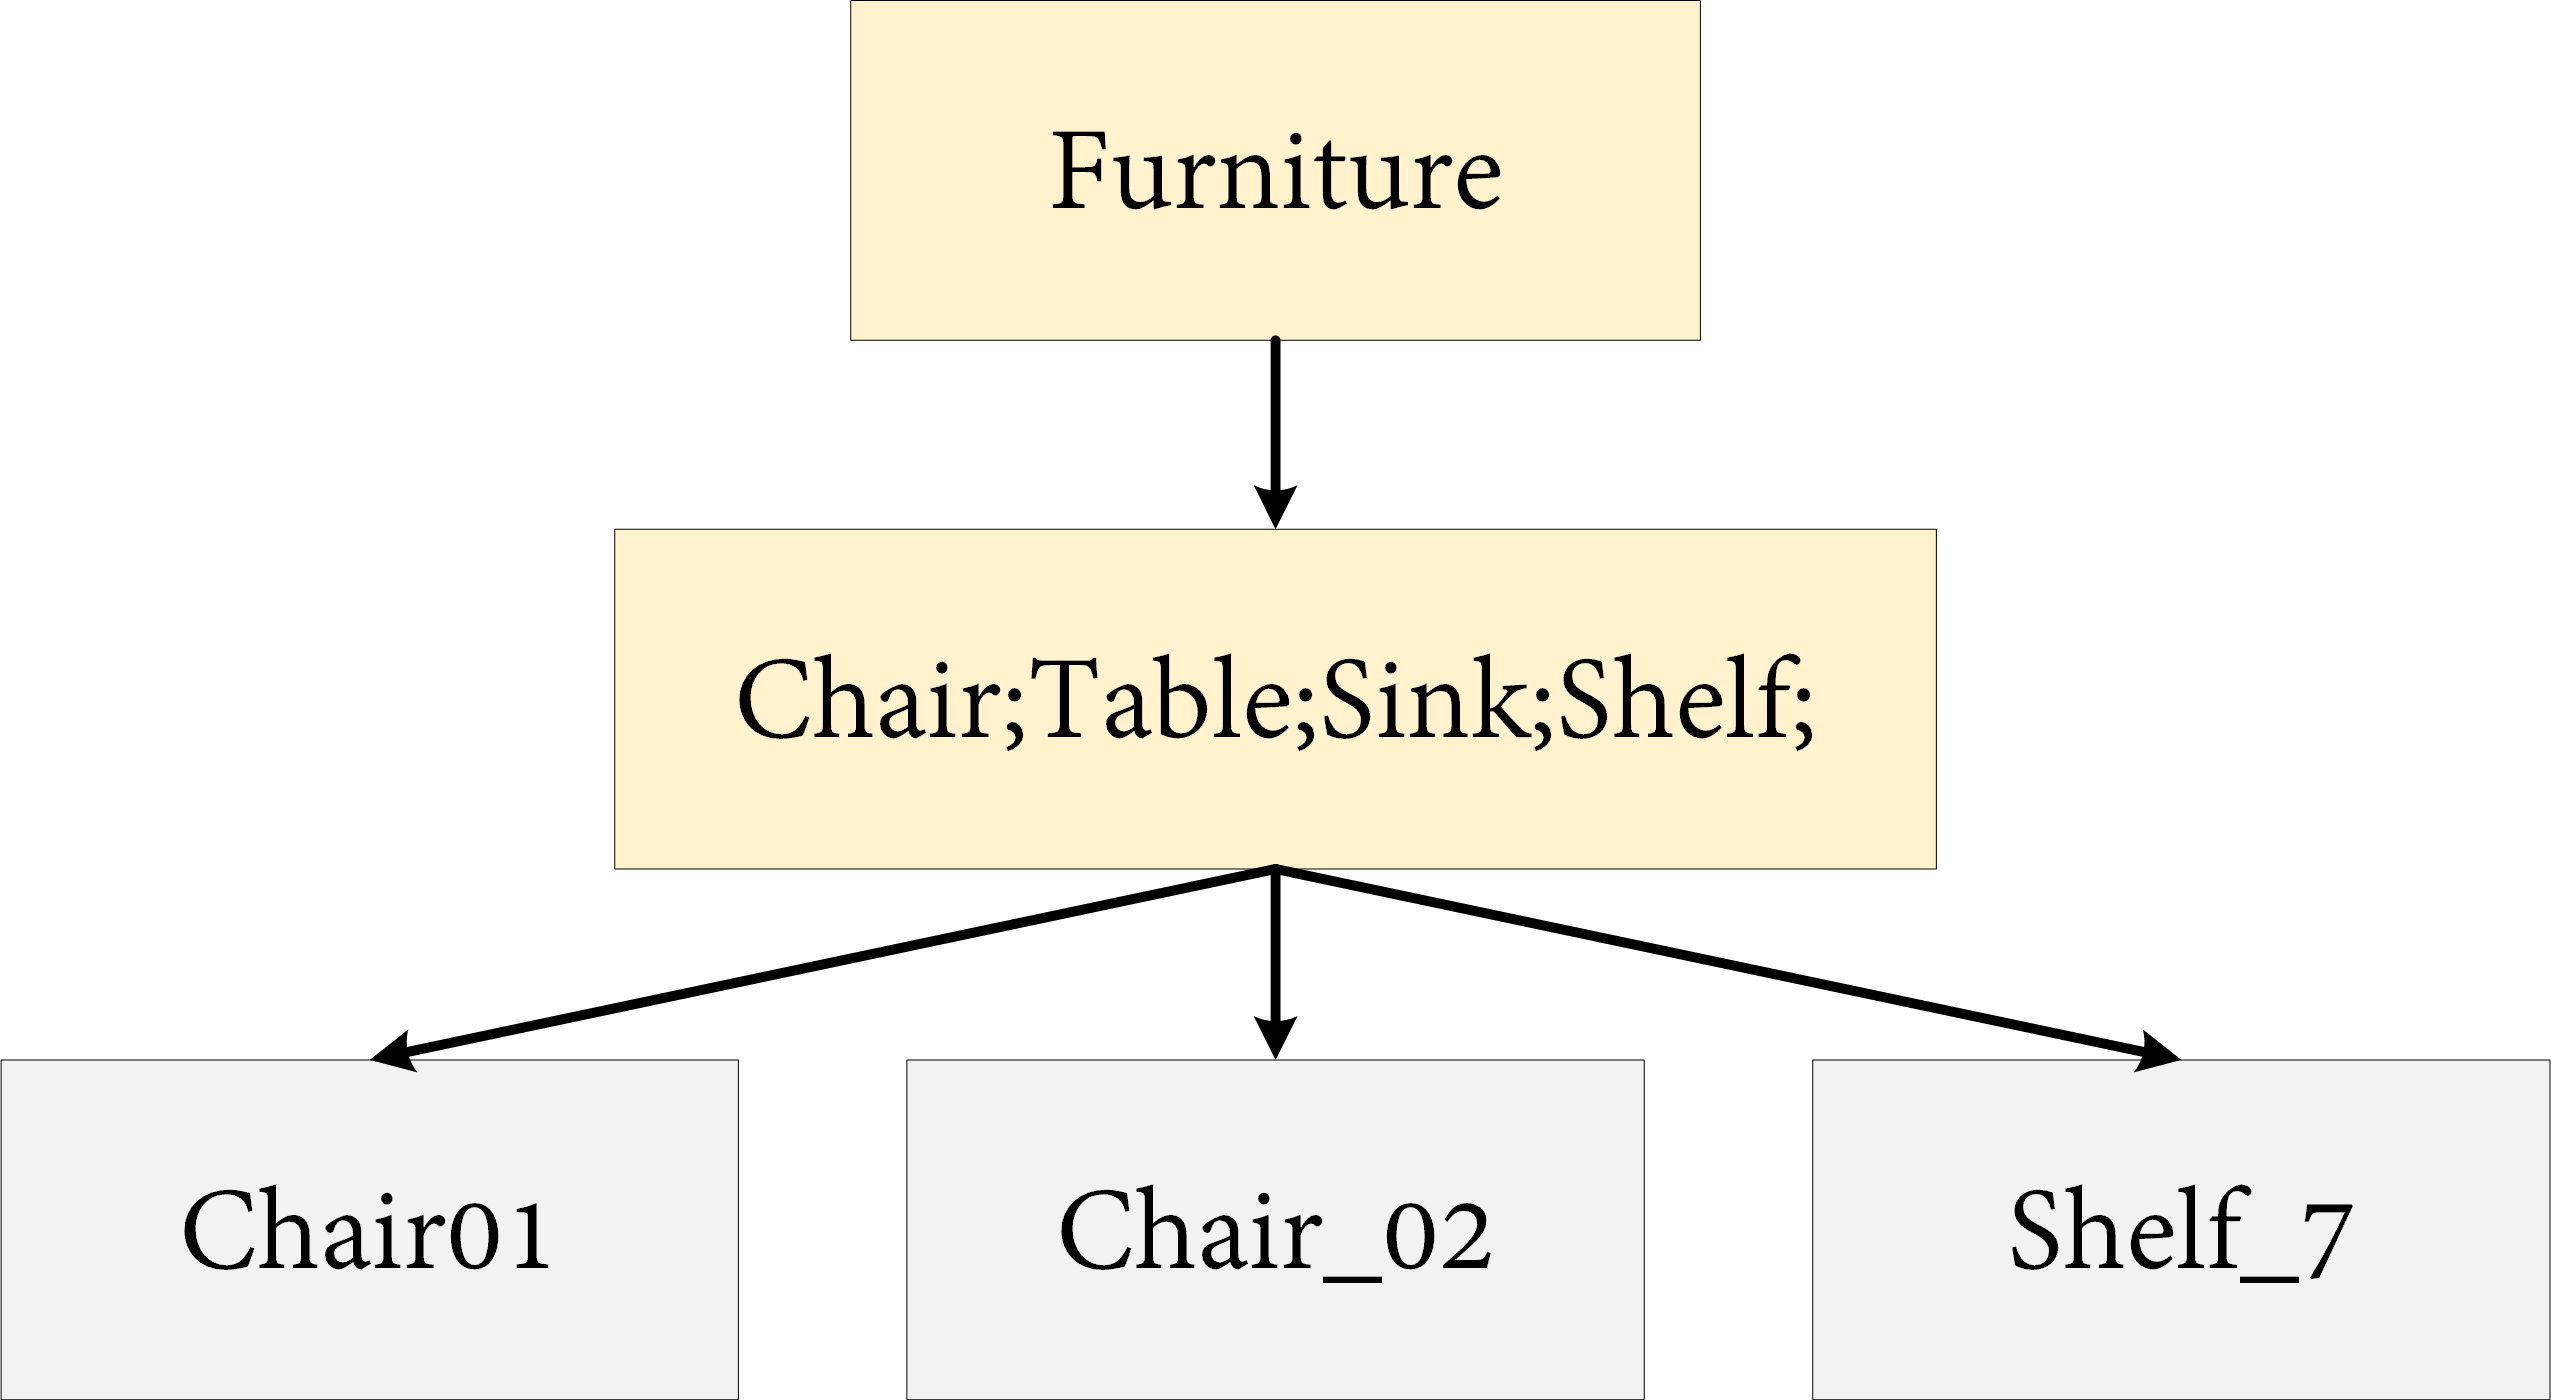
\includegraphics[width=\linewidth]{figs/lidar_simulation/semantic_labels_example.png}
	\caption{Example of hierarchical annotation, where the furniture label includes a wide range of items. }
	\label{fig:semantic_label_examples}
\end{marginfigure}
Instead of manually labelling large \acrshort{lidar} point clouds, human operators are required to label objects in a 3D triangle mesh. This task is facilitated using a hierarchical segmentation that is sped up using the naming conventions of objects and materials (see Figure \ref{fig:semantic_label_examples}). During the mesh loading, object names are considered significant whether they do not collide with other instances' names. Otherwise, they are named after the material together with a unique $\mathtt{id}$. Furthermore, models are organized either by following a custom tag or standard labels defined in the LASer (\acrshort{las}) file format (see Figure \ref{fig:kitchen_classification}). The former can be collapsed or further subdivided according to the required \acrshort{lod}, thus helping to provide a fine-grained segmentation. In contrast to the manual classification of real \acrshort{lidar} point clouds, annotated environments help to suppress labelling errors and provide a fine-grained segmentation. Otherwise, manual labelling should be limited to a few classes to avoid overwhelming human operators in this task.

\begin{figure}[ht]
    \centering
    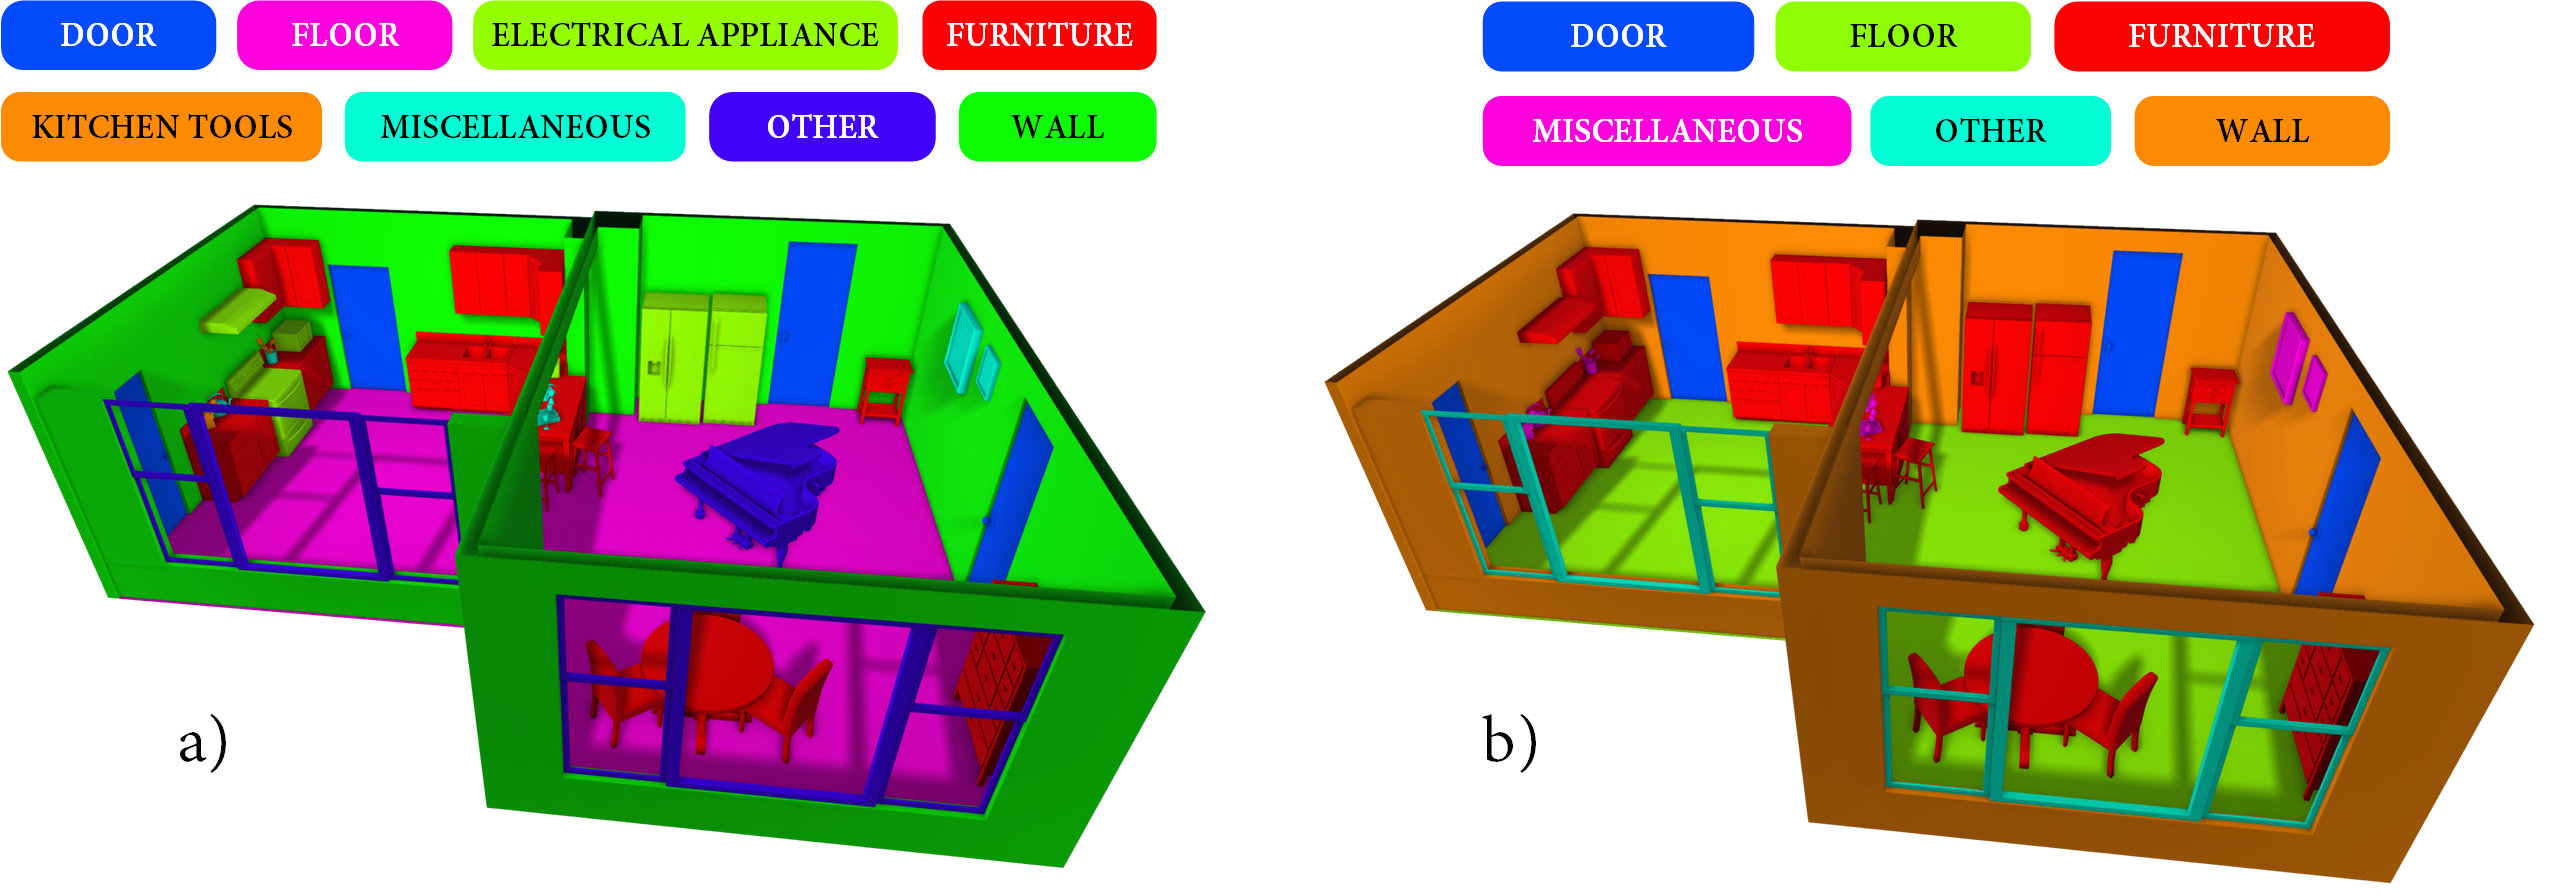
\includegraphics[width=\linewidth]{figs/lidar_simulation/semantic_labels.png}
	\caption{Different criteria for labelling a static scenario. First, the scene is annotated using custom labels, whereas the second classification is performed with semantic labels in the \acrshort{las} 1.4 standard.}
	\label{fig:kitchen_classification}
\end{figure}

Besides semantic labels, models are also linked to materials that help in computing the \acrshort{lidar} intensity. This property will be further described in the following chapter. Finally, the identifier of each instance is also stored to make the simulated datasets appropriate for instance segmentation.

\section{LiDAR simulation}

This section is structured according to the steps followed in the \acrshort{gpu}-based \acrshort{lidar} scans. First, a comprehensible explanation of \acrshort{lidar} pulse modelling is provided, followed by the interaction of \acrshort{lidar} beams and synthetic surfaces. The latter stage will also help to introduce the pipeline in the \acrshort{gpu}. The generic parameters used throughout this chapter are explained in Table \ref{table:lidar_workflow_parameters}. 

\renewcommand{\arraystretch}{1.2}
\begin{table*}
    \small
    \caption{Baseline configuration parameters of \acrshort{lidar} simulations. These parameters are in common to \acrshort{als} and \acrshort{tls}. }
    \label{table:lidar_workflow_parameters}
    \begin{tabular}{ll}
    \toprule
    \textbf{Parameter} & \textbf{Description}\\
    \midrule
    Wavelength ($\lambda$) & 532 \si{\nano\meter} for bathymetric scans, 1064 \si{\nano\meter} otherwise.\\
    Pulse radius ($r$) & Radius at a distance of $t = 1$ following the ray parametric equation. \\
    Rays per pulse ($n_{p}$) & \acrshort{lod} of the pulse discretization. \\
    Energy ($\bar{I}$) & Energy linked to a \acrshort{lidar} pulse, given in \si{\watt}. \\
    Sensor diameter ($p_{l}$) & Diameter of the \acrshort{lidar}'s receiver component (\si{\meter}). \\
    Maximum number of returns ($n_{r}$) & Number of maximum returns per pulse. \\
    Maximum range ($R$) & Maximum range covered by a single pulse.\\
    Fuzzy boundary around $R$ ($R_{\delta_{\textit{min}}}, R_{\delta_{\textit{max}}}$) & Fuzzy boundary to avoid abrupt losses when $R$ is reached.\\
    Terrain-induced error ($e_{\textit{terrain}}$) & Boolean value indicating if errors related to slopes are simulated. \\
    Shiny surface error ($e_{\textit{glossy}}$) & Boolean value indicating if the 'time-walk' effect is simulated. \\
    Outlier threshold ($t_{\textit{outlier}}$) & Probability of generating outliers. \\
    % Outlier range ($t_{\textit{min}}, t_{\textit{max}}$) & Dispersion of outliers. \\
    Atmospheric attenuation ($a_{\textit{atm}}$) & Atmospheric attenuation factor (see Equation \ref{eq:lidar_equation}). \\
    System transmission ($n_{\textit{sys}}$) & System transmission factor (see Equation \ref{eq:lidar_equation}). \\
    \bottomrule
    \end{tabular}
    \libertineNormal
\end{table*}
\renewcommand{\arraystretch}{1}

\subsection{Pulse modelling}

\acrshort{lidar} pulses are modelled as a set of rays emitted at the sensor's location that propagate towards uniformly sampled points in a unit sphere. From now on, the emitter and receiver will be assumed to be placed in the same location to simplify the conceptualization of the \acrshort{lidar} mechanism. Rather than a single ray, the physical behaviour of a \acrshort{lidar} pulse is better simulated with multiple rays \cite{zohdi_rapid_2020} (see Figure \ref{fig:pulse_radius_insight}) within a radius that can be static (collimated beams; parallel rays) or dynamic (diverging beams). Rays in the same pulse are calculated according to the orthonormal basis ($\hat{u}, \hat{v}, \hat{r}_{d}$) formed by the ray direction and the $\hat{\textit{up}}$ vector. $\hat{u}, \hat{v}$ are then scaled with random numbers to generate points within a circumference of radius $r$. 

\begin{figure}[ht]
	\centering
	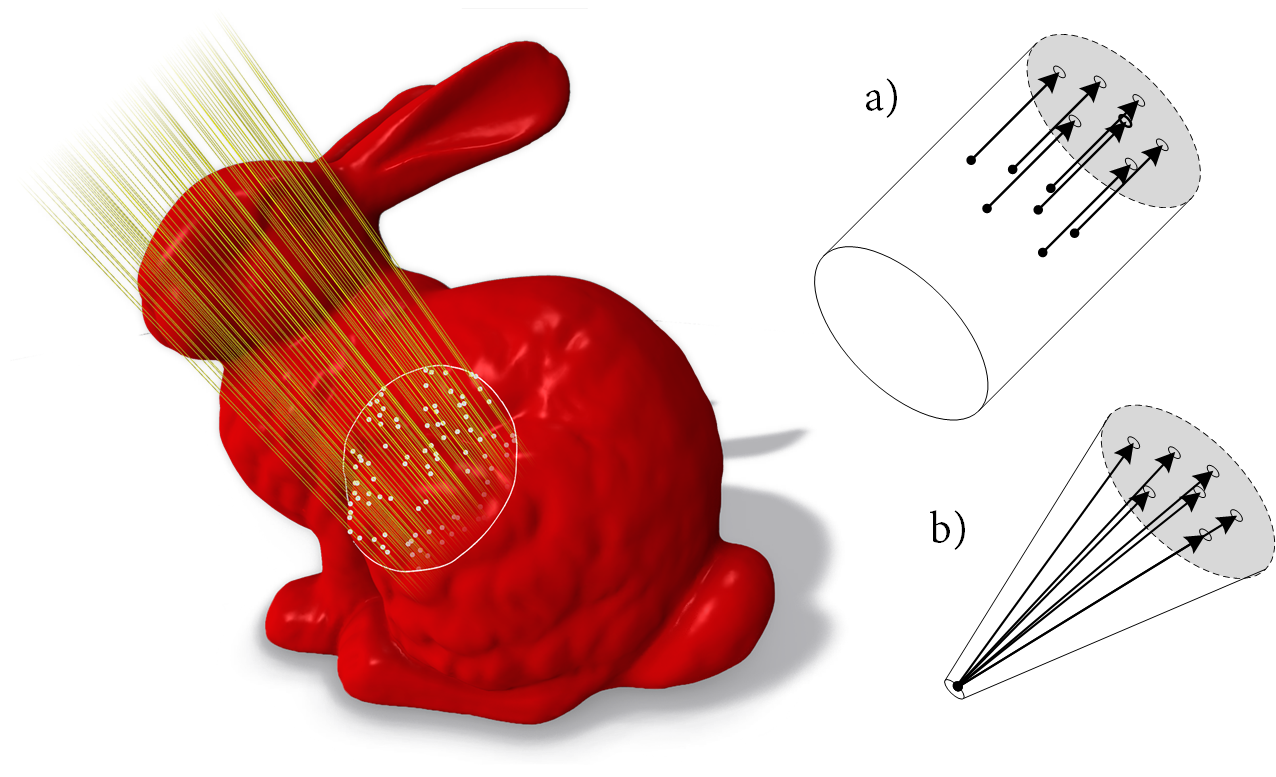
\includegraphics[width=\linewidth]{figs/lidar_simulation/ray_section.png}
	\caption{Collimated rays from the same pulse intersecting the Bunny model. The figures on the right side show the scheme of a) collimated rays and b) diverging rays.}
	\label{fig:pulse_radius_insight}
\end{figure}

\subsubsection{Terrestrial \acrshort{lidar} (\acrshort{tls})}

\renewcommand{\arraystretch}{1.2}
\begin{table*}
    \small
    \centering
    \caption{Parameters which can be configured on the propagation of laser beams from \acrshort{tls}. Position-related factors are expressed in \si{\meter}, whereas angular parameters are expressed in radians.}
    \label{table:tls_parameters}
    \begin{tabular}{ll}
    \toprule
    \textbf{Parameter} & \textbf{Description} \\
    \midrule
    Position ($p$) & Position of \acrshort{lidar}'s emitter.\\
    Field of view ($\alpha_{\textit{fov}_{xz}}$, $\alpha_{\textit{fov}_{y}}$) & Horizontal and vertical aperture ($0 \leq \alpha_{\textit{fov}_{xz}} \leq 2\pi$ and $0 \leq \alpha_{\textit{fov}_{y}} \leq \pi$). \\
    Scanning resolution ($r_{x}$) & Number of horizontal scan lines. \\
    Horizontal reference angle ($\alpha_{\textit{centre}_{xz}}$) & It helps to calculate the starting horizontal angle as $\alpha_{\textit{centre}_{xz}} - \alpha_{\textit{fov}_{xz}} / 2$. \\
    Vertical reference angle ($\alpha_{\textit{centre}_{y}}$) & It helps to calculate the starting vertical angle as $\alpha_{\textit{centre}_{y}} - \alpha_{\textit{fov}_{y}} / 2$. \\
    The number of channels ($n_{c}$) & Number of simultaneous channels. \\
    Channel spacing ($d_{c}$) & Interleaved distance between consecutive channels.\\
    Channel angular distance ($d_{\alpha_{c}}$) & Interleaved emission angle between consecutive channels.\\
    Axis noise ($\hat{\delta}_{\textit{noise}}$) & Magnitude of ray jittering. \\
    Angle noise ($\alpha_{\textit{noise}}$) & Magnitude of the angle used for jittering the ray's target position. \\
    \bottomrule
    \end{tabular}
    \libertineNormal
\end{table*}
\renewcommand{\arraystretch}{1}

The parameters concerning \acrshort{tls} simulations are described in Table \ref{table:tls_parameters}. Rays in \acrshort{tls} spread in a sphere which is discretized through the horizontal and vertical resolution, $r_x$ and $n_c$. Furthermore, horizontal and vertical \acrshort{fov} determine which part of the sphere is covered, since these angles can be lower than $2\pi$ and $\pi$, respectively. The \acrshort{fov} is parameterized with $\alpha_{\textit{centre}_{xz}}, \alpha_{\textit{fov}_{xz}}$ as well as $(\alpha_{\textit{centre}_{y}}, \alpha_{\textit{fov}_{y}})$. Therefore, the horizontal \acrshort{fov} covers $[\alpha_{\textit{centre}_{xz}} - \frac{\alpha_{\textit{fov}_{xz}}}{2}, \alpha_{\textit{centre}_{xz}} + \frac{\alpha_{\textit{fov}_{xz}}}{2}]$, whereas the spacing of channels is $d_c$ (by default, it is almost zero, $\epsilon \gets 1^{-16}$). However, this ideal spatial subdivision leads to grid-like renderings (Moiré effect) of \acrshort{lidar} point clouds, which can be interpreted as an artefact. Instead, this unwanted visual effect can be avoided by jittering \cite{akenine-moller_real-time_2018} the emitted rays, thus leading to an imperfect result. Furthermore, it enables emulating beam jittering and minor inaccuracies as a result of the limited sensor accuracy \cite{mcmanamon_lidar_2019}. The jittering changes both the ray's direction ($\hat{\delta}_{\textit{noise}}$) and its magnitude ($\alpha_{\textit{noise}}$) with random values in $[-1, 1]$.

\begin{figure}[ht]
	\centering
	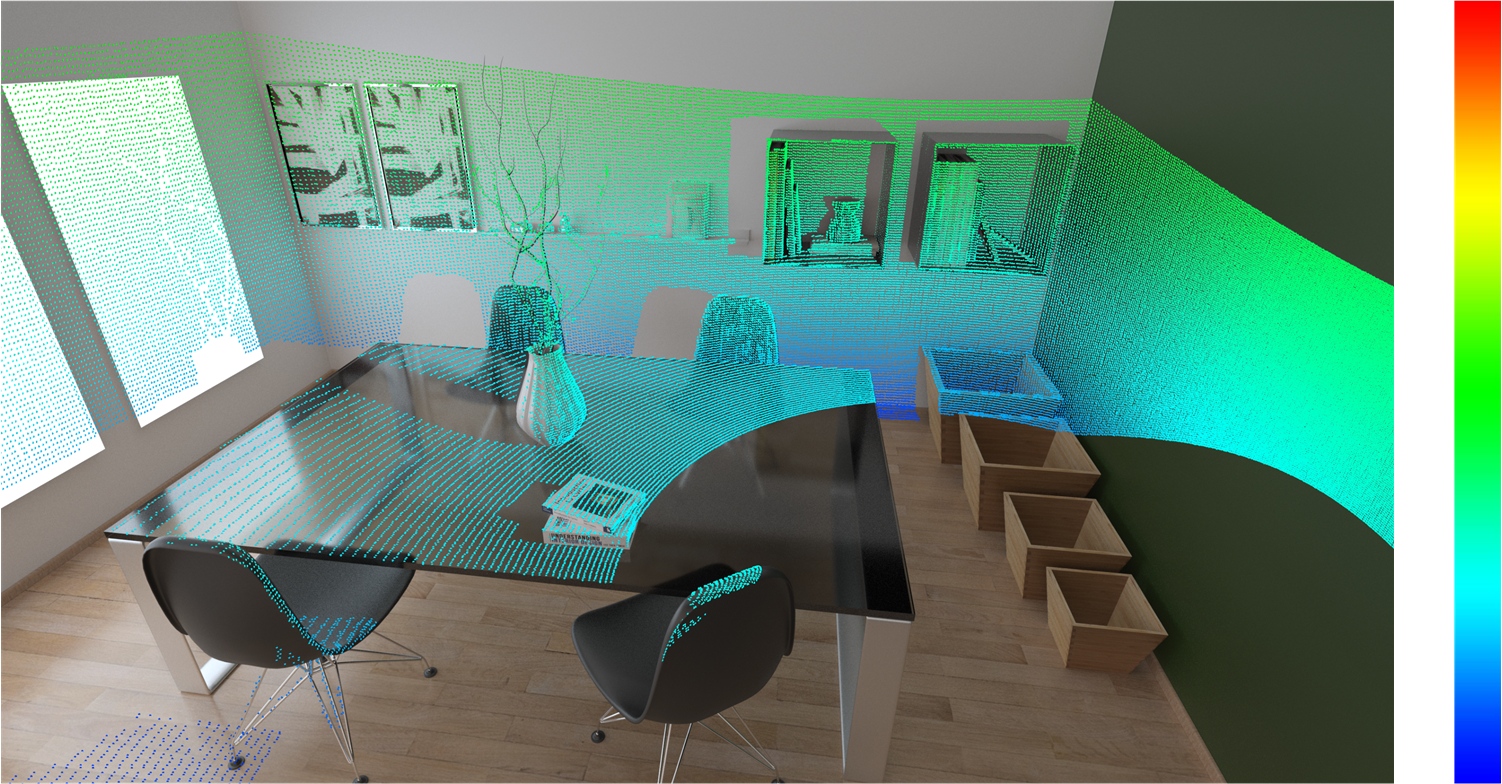
\includegraphics[width=\linewidth]{figs/lidar_simulation/tls_first_approach.png}
	\caption{Terrestrial scan with point colours encoding their relative height.}
	\label{fig:tls_first_approach}
\end{figure}

Equation \ref{eq:ray_target_tls} shows the scattering direction of a beam emitted from the \acrshort{tls}'s emitter (Equation \ref{eq:ray_origin_tls}). Horizontal lines ($\alpha_{xz}$) enable calculating the position $\Theta$ on the surface of a unit sphere with $y \gets 0$, whereas the vertical lines ($\alpha_{y}$) determine the elevation of such point. Also note that $s_{d}$ and $\hat{\delta}_{xyc}$ are defined as orthogonal vectors from Equation \ref{eq:sphere_point_tls}. $r(u)$ shows the ray equation expressed through its origin, $r_{o}$, and target point, $r_{t}$. 
\begin{align*}
    &r_{o} = p + \left[0, \frac{-d_{c}\left(n_{c} - 1\right)}{2} + c d_{c}, 0\right]^\intercal 
    \numberthis \label{eq:ray_origin_tls}\\
    &r_{t} = r_{o} + \Omega_{1}\left(\hat{\delta}_{\textit{noise}}\begin{bmatrix}\lambda_{x} \\ \lambda_{y} \\ \lambda_{z} \end{bmatrix}, \alpha_{\textit{noise}}\lambda_{\alpha}\right) \Omega_{2}\left(\hat{\delta}_{xyc}, \alpha_{y}\right) \Theta
    \numberthis \label{eq:ray_target_tls}\\[.4em]
    &r(u) = r_o + u\widehat{\left(r_{t} - r_{o}\right)}
    \numberthis \label{eq:ray_equation_tls}
\end{align*}
where intermediate results are calculated as follows:
\begin{align*}
    \Theta &= \left[\cos{\alpha_{xz}}, 0, -\sin{\alpha_{xz}}\right]^\intercal 
    \numberthis \label{eq:sphere_point_tls}\\
    \hat{\delta}_{xyc} &= \left[\Theta_{z}, 0, -\Theta_{x}\right]^\intercal
    \numberthis \label{eq:sphere_angle_tls}\\
    \alpha_{xz} &= \alpha_{\textit{centre}_{xz}} - \frac{\alpha_{\textit{fov}_{xz}}}{2} + \alpha_{\textit{fov}_{x}}\left(\frac{x}{r_{x}} + \frac{y}{ r_{x}n_{c}} - \frac{1}{2}\right)
    \numberthis \label{eq:horizontal_angle_tls}\\
    \alpha_{y} &= \alpha_{\textit{centre}_{y}} - \frac{\alpha_{\textit{fov}_{y}}}{2} + y\left(\frac{n_{c}\alpha_{\textit{fov}_{y}} + \alpha_{\textit{fov}_{y}}}{{n_{c}}^2}\right)
    \numberthis \label{eq:vertical_angle_tls}
\end{align*}
provided that $\Omega$ represents a rotation matrix defined by a rotation axis and scalar angle, whereas $\lambda_{x}$, $\lambda_{y}$, $\lambda_{z}$ and $\lambda_{a}$ are random values generated through a random uniform distribution. $x$ and $y$ are iterative values so that $0 \leq x < r_{x}$, $0 \leq y < n_{c}$. $\alpha_{xz}$ and $\alpha_{y}$ are horizontal and vertical angles, respectively. Accordingly, $0 \leq \alpha_{xz} \leq 2\pi$ and $\frac{-\pi}{2} < \alpha_{y} < \frac{\pi}{2}$. 

Furthermore, other \acrshort{lidar} models such as Pandar64 do not have uniform resolution along the vertical axis \cite{hesai_pandaset_2021}. To cope with this kind of sensor, several intervals can be defined with the starting and limit angles.  

Even this straightforward construction of \acrshort{tls} rays has a significant latency in high-resolution scans covering large areas. Thus, this construction stage was solved with a massively parallel approach in the \acrshort{gpu} to handle every ray with a different thread, rather than in a sequential manner. In contrast to the \acrshort{cpu}, one of the main drawbacks of \acrshort{gpgpu} is the lack of noise functions required for randomizing the ray generation. Some pseudo-random generators are frequently used in \acrshort{glsl}, though noise was required to be uniformly distributed. This was solved by building a large buffer with uniform random values computed in the \acrshort{cpu}, which are later used by \acrshort{gpu} threads to randomize \acrshort{lidar} simulations. Another challenge arises from the limited \acrshort{gpu} memory since \acrshort{ssbo}s expand to a few gigabytes at most, regardless of the \acrshort{gpu} capacity. Therefore, the ray generation is split into several iterations that overwrite a single \acrshort{ssbo} on which rays are stored, with each iteration being followed by the collision solver. Otherwise, \acrshort{cpu} and \acrshort{gpu} transfers would be larger to avoid exceeding the maximum capacity. The maximum number of allocatable rays in a single buffer is computed from the maximum capacity of an \acrshort{opengl}'s \acrshort{ssbo}, the size of a single ray and the number of rays within a pulse, $n_p$, as shown in Equation \ref{eq:max_rays_ssbo}. Note that rays within a pulse cannot be separated into different iterations since they behave synchronously.
\begin{equation}
    \label{eq:max_rays_ssbo}   
    n = n_p\lfloor{\frac{\mathtt{\tiny{glGetIntegerv(GL\_MAX\_SHADER\_STORAGE\_BLOCK\_SIZE)}}}{n_p \cdot \tiny{\mathtt{sizeof(Ray)}}}\rfloor}
\end{equation}

\subsubsection{Aerial \acrshort{lidar} (\acrshort{als})}

\renewcommand{\arraystretch}{1.2}
\begin{table}
    \footnotesize
    \caption{Parameters which can be configured for generating rays from an \acrshort{als}. Again, angles are expressed in radians.}
    \label{table:als_parameters}
    \centering
    \begin{tabular}{ll}
    \toprule
    \textbf{Parameter} & \textbf{Description} \\
    \midrule
    Platform altitude ($h$) & Fixed elevation of the mobile platform.\\
    Field of view ($\alpha$) & Aperture of \acrshort{lidar} sensor. \\
    Speed of the platform ($\nu$) & Pace of the mobile platform in \si{\meter/\second}. \\
    Number of scans ($\xi$) & Number of scan lines per second. \\
    Number of pulses ($\psi$) & Number of pulses per second. \\
    Spatial noise ($\delta_{\textit{noise}}$) & Magnitude of distortion applied to the ray's target.\\
    Altitude noise ($h_{\textit{noise}}$) & Magnitude of jittering in the platform altitude.\\
    Scanning pattern & Pattern used to scan the scene. \\
    Flattening of ellipses ($e_{f}$) & $y$-scale of ellipses (elliptical scan pattern). 
    \\
    Radius of ellipses ($e_{r}$) & Radius of ellipses in the slanted pattern.\\
    \bottomrule
    \end{tabular}
\end{table}
\renewcommand{\arraystretch}{1}

\acrshort{tls} was explained so that beams were emitted from a single emitter location. However, both \acrshort{tls} and \acrshort{als} can be configured to follow a path, thereby simulating terrestrial and aerial vehicles, respectively. However, the configuration of airborne paths is slightly more complex, though they can be automatically computed, and thus will be introduced with \acrshort{als}. The parameters concerning \acrshort{als} that will be used throughout this section are described in Table \ref{table:als_parameters}.

In comparison with \acrshort{tls}, \acrshort{als} pulses a spread over a plane rather than a sphere, and the sensor's emitter changes according to the path. Among other features, the \acrshort{fov} is typically narrowed to avoid including returns from atmospheric particles, and yet, noisy returns are very frequent. In this case study, the jittering affects the emitted rays and the height of the mobile platform, with a magnitude of $\delta_{\textit{noise}}$ and $h_\textit{noise}$, respectively. The resolution is parameterized by the number of scans and pulses per second. Instead of only performing parallel scans, other patterns are frequently used in \acrshort{als} to maximize the point cloud coverage. Figure \ref{fig:als_patterns} shows the aftermath of zigzag and elliptical patterns \cite{dong_lidar_2018}. Hence, the configuration of \acrshort{als} includes parameters that help to automatize the estimation of the platform path. Regardless of the scanning pattern, the airborne platform moves according to such a path, and therefore, the emitter location is calculated with a parametric value, $t_i$. On the other hand, $r_d$ and $r_t$ are computed according to the scanning pattern and $t_i$. The rays emitted with parallel and zigzag patterns are calculated as follows:
\begin{align*}
    r_{o} &= p_{t_{i}} + 
    \begin{bmatrix} 0 \\ \lambda_{h}h_{\textit{noise}} \\ 0 \end{bmatrix} + \frac{\xi p_{s_{i}}}{\psi} \vec{d}
    \numberthis \label{eq:ray_origin_als_zigzag}\\
    r_{t} &= r_{o} - \hat{\delta}_{sp} \sin{\beta} +
    \begin{bmatrix}0 \\ -\cos{\beta}\\ 0 \end{bmatrix} + \delta_{noise}\vec{\lambda}
    \numberthis \label{eq:ray_target_als_zigzag}
\end{align*}
with the rotation angle $\beta$ and the vector $\delta_{sp}$ being:
\begin{align*}
    \beta &= \textit{z}_{s}\alpha \left(\frac{p_{s_{i}} \xi}{\psi} - \frac{1}{2}\right)
    \numberthis \label{eq:beta_als_zigzag}\\[0.4em]
    \delta_{sp} &= \left[-\vec{d}_{z}, 0, \vec{d}_{x}\right]^\intercal
    \numberthis \label{eq:rotation_axis_als_zigzag}
\end{align*}
given that $p_{s_{i}}$ is the index of a pulse within the $\textit{i}$-th sweep, $\vec{d}$ is the vehicle direction, $\delta$ is a random value and $\vec{\lambda}$ is a random vector, both retrieved from a uniform distribution and finally, $s$ is an iterative value such that $0 \leq s < \xi$. On the other hand, $\textit{z}_{s} \in \{-1, 0, 1\}$ enables omitting the program branching for parallel scanning ($\textit{z}_{s} \gets 0$), whereas -1 and 1 are used for odd and even iterations in the zigzag pattern.

\begin{figure}
    \centering
    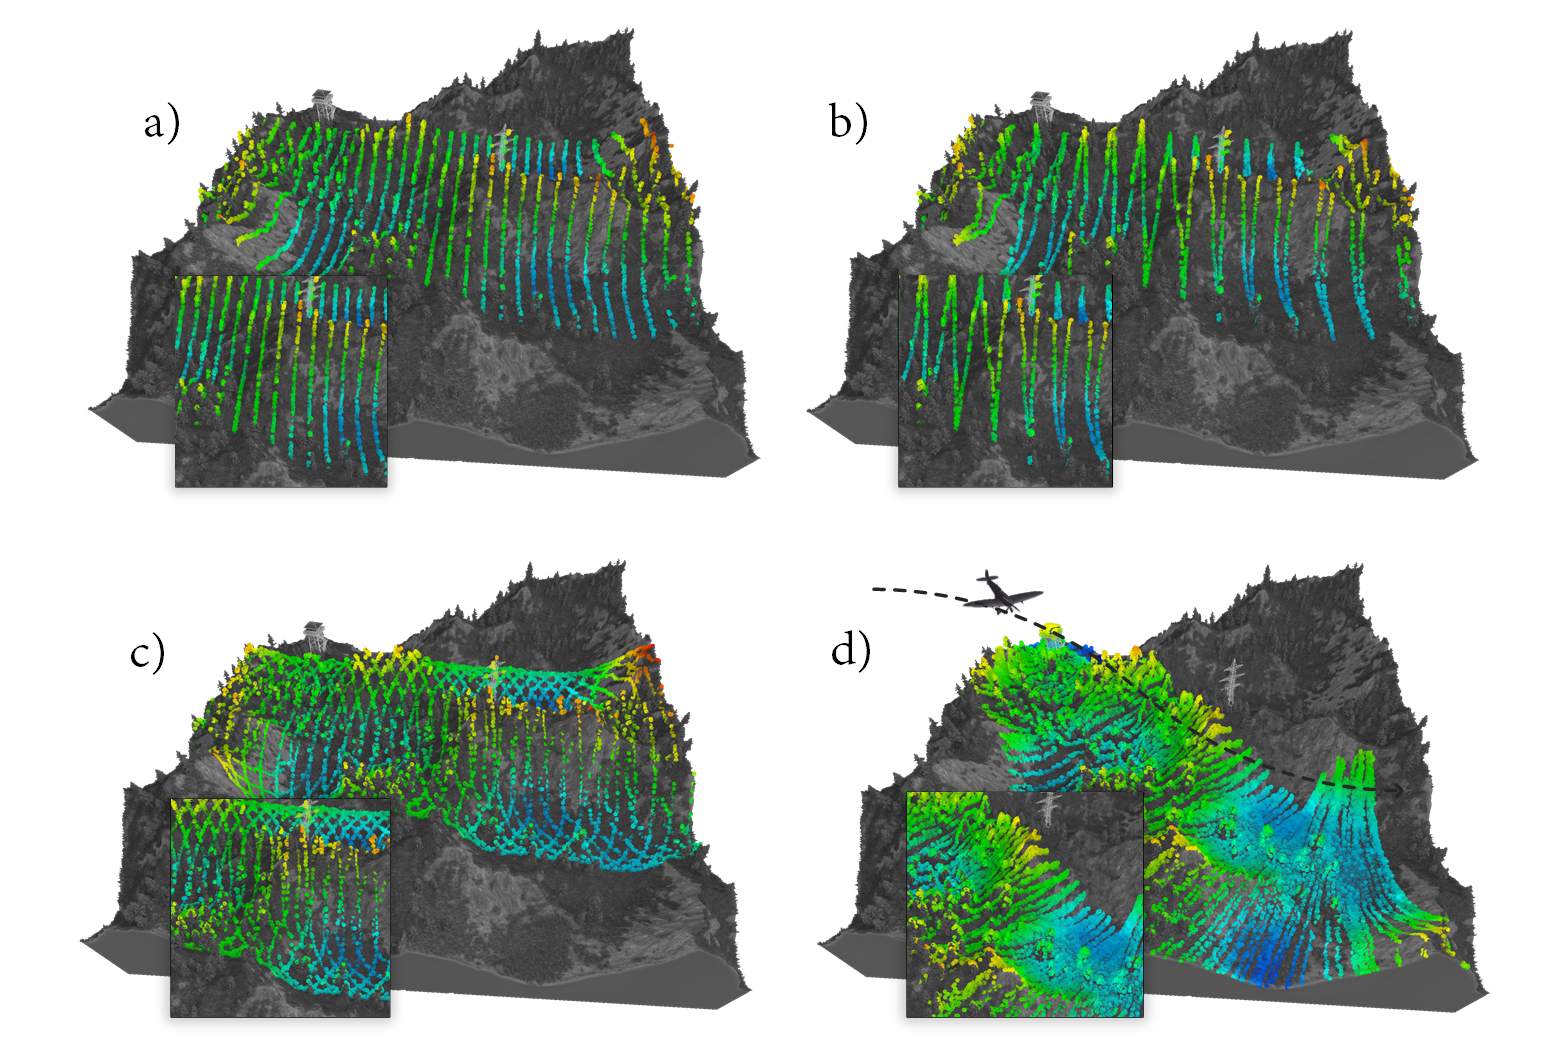
\includegraphics[width=\linewidth]{figs/lidar_simulation/als_patterns.png}
	\caption{Multiple airborne scans following a) parallel, b) zigzag and c) elliptical patterns. d) illustrates a custom path defined by the user in the \acrshort{gui}. }
	\label{fig:als_patterns}
\end{figure}

The elliptical pattern is slightly different as scans are now ellipses flattened with a factor $e_{f}$ (Equation \ref{eq:ray_target_als_elliptical}). Accordingly, $\beta$ defines a circumference flattened in the $x$-axis and centred in $p_{t_{i}}$. 
\begin{align*}
    r_{t} &= r_{o} + 
    \begin{bmatrix}e_{f} e_{r} \sin{\vartheta}\\ -h\\ e_{r} \cos{\vartheta}\end{bmatrix} + \delta_{\textit{noise}} \vec{\lambda}
    \numberthis \label{eq:ray_target_als_elliptical}
\end{align*}
where the rotation angle, $\vartheta$, and the ellipse radius, $e_{r}$, are calculated in Equations \ref{eq:beta_als_elliptical} and \ref{eq:radius_als_elliptical}.
\begin{align*}
    \vartheta &= \frac{2 p_{s_{i}} \pi \frac{\textit{aabb}_{x}}{s_{p} \xi}}{\frac{\textit{aabb}_{x}}{s_{p} \psi}} = \frac{2 p_{s_{i}} \pi \psi}{\xi} 
    \numberthis \label{eq:beta_als_elliptical}\\[0.4em]
    e_{r} &= h \tan{\frac{\alpha}{2}}  
    \numberthis \label{eq:radius_als_elliptical}
\end{align*}
Intuitively, $e_{r}$ is computed with the tangent of $\frac{\alpha}{2}$ for any height $h$. The formulae were considerably simplified by momentarily assuming that $h \gets 1$, and therefore, $r_{d_{y}} \gets -h$. On the other hand, $i$ is defined as the index of each incremental step, related to the parametric value $t_{i}$.

Scenarios can be scanned with \acrshort{als} following parallel routes along the $X$ or $Z$ axis. Platform rotations involving changes in the $\textit{forward}$ direction are not simulated since these waypoints are typically discarded in post-processing. Hence, computer-aided paths simply consist of sparse lines parallel to the $X$-axis. The distance between them is calculated considering the dimensions of the scenario as well as the sensor's \acrshort{fov} (Equation \ref{eq:num_aerial_sweeps}), in order to exhaustively cover the scene. Otherwise, the path can be defined using a canvas in the \acrshort{gui}, though these require further processing. User-defined paths comprise points recorded in every frame as long as the painting pointer is being dragged, thereby generating paths with a huge number of (noisy) points. This shortcoming was tackled by simplifying the path with the Douglas-Pecker algorithm \cite{douglas_algorithms_1973}: the path remains very similar, whereas the number of points is significantly lowered and the noise is mitigated. Then, points in this path are the control points of a Catmull-Rom spline which will be later sampled during the scan. Either computer-aided or defined by users, paths are sampled in the \acrshort{cpu} and transferred to the \acrshort{gpu} to make this routine simpler in the \acrshort{gpu} processing. 
\begin{equation}
    n_{\textit{steps}} = \lceil{\frac{\textit{aabb}_{\textit{min}_z}}{2(h - \textit{aabb}_{\textit{min}_y})\tan(\frac{\alpha}{2})}\rceil}
    \numberthis \label{eq:num_aerial_sweeps}
\end{equation}
where $\textit{aabb}_{\textit{min}}$ is the minimum point of the scene's \acrshort{aabb}.

Finally, the emitted rays in \acrshort{als} change considerably with respect to \acrshort{tls}; firstly, diverging laser beams within a pulse were simulated instead of collimated beams, as proposed by Zohdi \cite{zohdi_rapid_2020}. Given a radius $r$ defined at a distance $d \gets 1$, rays are scattered following the Equation \ref{eq:ray_target_diverging}. For each ray, an orthonormal basis is constructed ($\hat{u}, \hat{v}, \hat{r}_{d}$) using the ray direction, $r_{d}$, as well as an up vector, $\widehat{\textit{up}}$, expressed as $\left[0, 1, 0\right]^\intercal$ for \acrshort{tls}. Accordingly, $\hat{u}, \hat{v}$ correspond to the $X$ and $Y$ axes in the ray coordinate system, and therefore, scaling both vectors by a random factor $\delta_{r} \in [-r, r]$ and adding them to the ray's target ($r_{t}$) leads to a diverging beam. For that purpose, the point calculated in Equation \ref{eq:ray_target_diverging}, $p_{d_{i}}$, satisfies $\lVert p_{d_{i}} - r_{t}\rVert < r$, provided that $i$ is bounded by the number of rays in a pulse, $n_{p}$, and the distance is measured by a simple Euclidean function. Consequently, \acrshort{lidar} simulations are more precise with larger values of $n_{p}$, despite having a higher memory footprint.
\begin{gather}
    \label{eq:ray_target_diverging}
    \begin{aligned}
        p_{d_{i}} &= r_{o} + \hat{r}_{d} + \hat{u}\delta_{r} + \hat{v}\delta_{r} = r_{t} + \hat{u}\delta_{r} + \hat{v}\delta_{r}\\
        \vec{u} &= \widehat{\textit{up}} \times \hat{n}\\
        \vec{v} &= \hat{n} \times \hat{u}
    \end{aligned}
\end{gather}

\subsection{Collision solver}

\acrshort{tls} and \acrshort{als} rays interact with surfaces to construct dense synthetic point clouds enhanced with semantic information. The emitted rays operate following the synchronous stages shown in Figure \ref{fig:lidar_workflow}, regardless of the scanning platform. Particularities on \acrshort{tls} and \acrshort{als} can be implemented through shader subroutines rather than different pipelines. The \acrshort{gpu}-based stages are explicitly synchronized to avoid simultaneous reading and writing operations from different steps. Stages involving randomness use buffers generated with a custom random distribution and accessed with an offset equal to the thread index. The \acrshort{qmc} (Quasi-Monte Carlo) Halton sampler was used along with the C++ built-in uniform random distribution, although other samples could be integrated. The number of rays processed during a single iteration must be a multiple of $n_{p}$.

The stages depicted in Figure \ref{fig:lidar_workflow} are following described:
\subsubsection{Ray initialization}

Initially, rays carry a value of energy equal to $\bar{I} / n_{p}$, with $\bar{I}$ being the energy of a single pulse in watts (\si{\watt}). The return number is set to zero and the refractive index is initially one (air medium). 

\begin{marginfigure}[-4.0cm]
	\centering
	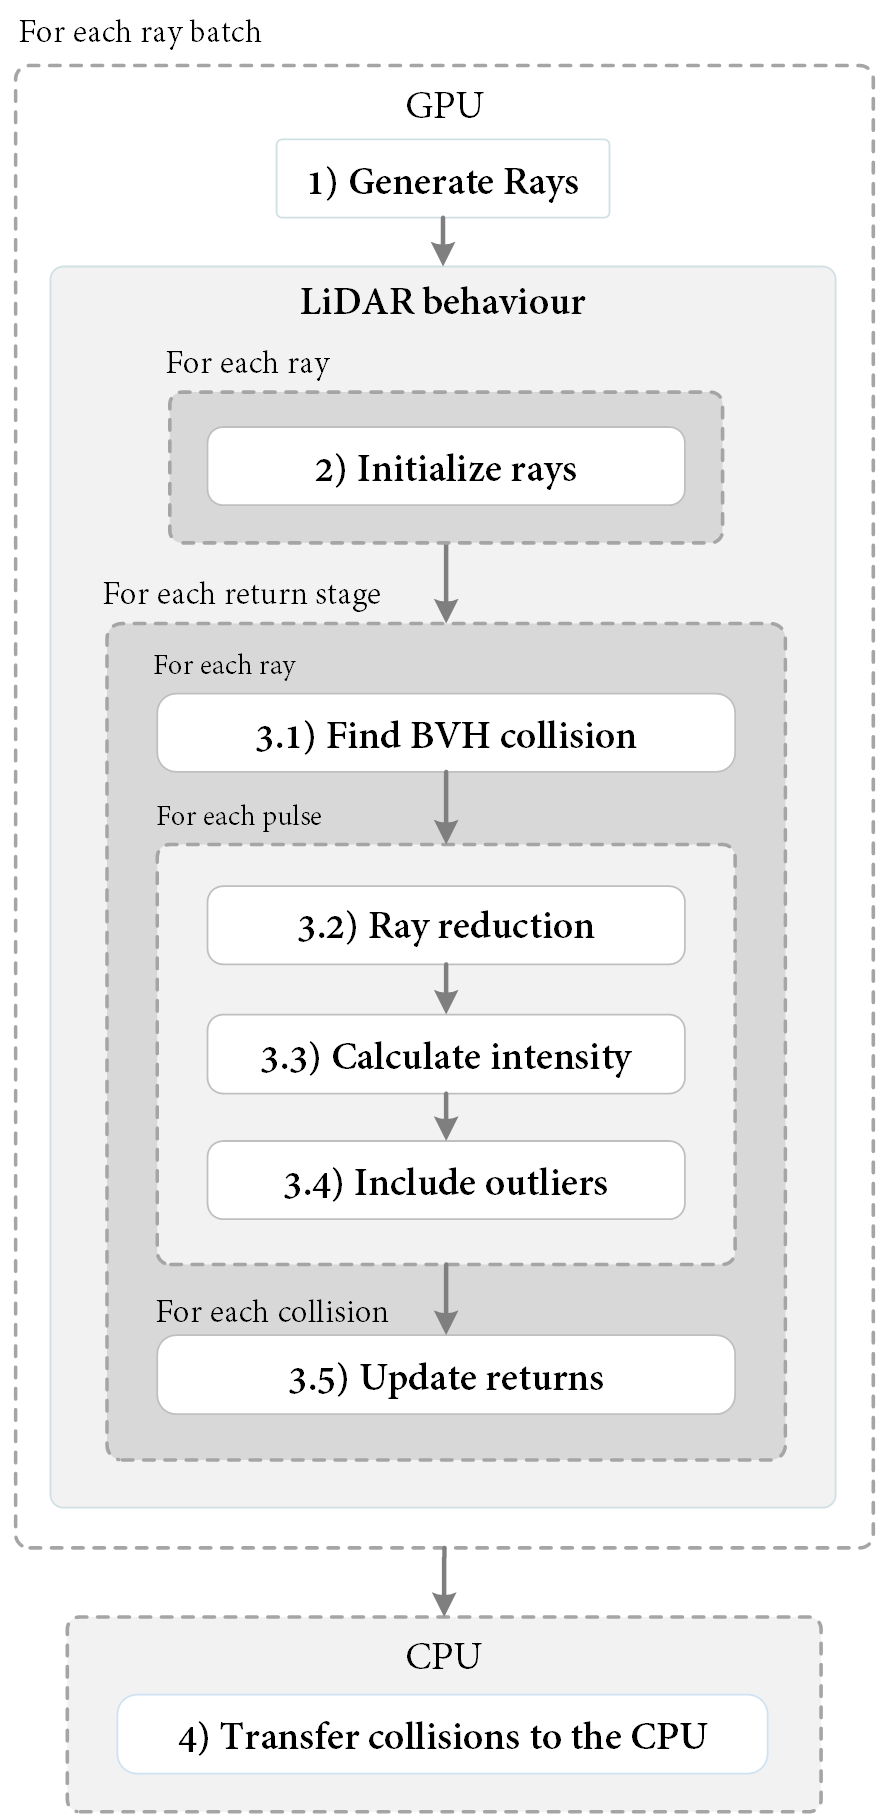
\includegraphics[width=\linewidth]{figs/lidar_simulation/lidar_overview.png}
	\caption{Summary of the simulation workflow as implemented in the \acrshort{cpu} and \acrshort{gpu}. \acrshort{cpu} processing is minimized during this pipeline to avoid delays from data transfers.}
	\label{fig:lidar_workflow}
\end{marginfigure}

\subsubsection{Find collision in the \acrshort{bvh}}

Each ray finds the nearest intersected polygon and surface. This stage requires the constructed \acrshort{bvh} as well as solving ray-\acrshort{aabb} and ray-triangle intersections. The foundational core is the time-of-flight (\acrshort{tof}) principle, which involves estimating the nearest intersection by timing the travel distance of the laser beam, whose velocity is known. Whether the propagated ray detects an intersection, the indices of the intersected triangle and surface are stored in what is called a collision buffer. 

\subsubsection{Ray reduction}

Then, rays do not operate individually but rather as a group of rays in a pulse. Hence, the number of shader calls is $p$ instead of $n_{p}p$. This stage helps to simulate multiple returns since rays which are not terminated early are able to penetrate high and low vegetation and acquire ground-labelled points. Although a pulse can detect several, disparate returns, only one is considered valid at each incremental step. Therefore, threads that intersected the nearest surface or did not collide are terminated, whereas the rest continue their path. Several impacts are considered to belong to the same chunk of a surface if multiple criteria are met. 
\marginnote[5.0cm]{
    Measuring the distance solely with $2dr + \epsilon$ leads to omitting those collisions whose $\hat{n} \cdot \hat{r}_{d}$ highly differs from 1. Consequently, the maximum distance is corrected as shown in Equation \ref{eq:pulse_radius_slope_distance}.
}
\begin{itemize}
    \item Collisions fall in the same triangle. This assumption cannot be applied to objects, since triangle meshes represented by several not-enclosed surfaces, such as leaves, may lead to missing some returns.
    \item Distance among collisions is smaller than $2 - \left|\hat{n} \cdot \hat{r}_{d}\right|$, thus taking into account the surface normal vector. Accordingly, this condition is expressed as shown in Equation \ref{eq:pulse_radius_slope_distance}, given that $d$ is the distance from the collision to the \acrshort{lidar}'s receiver component, $r$ is the pulse radius and $\hat{n}$ is the surface normal.
    \begin{equation}
        \label{eq:pulse_radius_slope_distance}
        d_{\textit{max}} = 2dr \cdot (2 - \left|\hat{n} \cdot \hat{r}_{d}\right|)
    \end{equation}
    \item Collided triangles are adjacent and therefore they share at least two vertices. Given the limited radius of a single pulse, checks of one-level depth are sufficient under the majority of scenarios.
\end{itemize}

Rays change based on the conclusions that were extracted in this section: those that collided with a surface which was not the closest one follow their path, in contrast to those that did not collide or caused the current return. Consequently, laser emissions may iteratively find several returns, and each new intersection is assigned a return number that is later completed with the number of collisions returned per pulse at the end of the simulation. 
  
% On the other hand, returns can also be discarded if the distance to the sensor's emitter is higher than $R$. The slope of surfaces influences the distortion of returned collisions, both on vertical and horizontal axes \cite{deems_lidar_2013}. The magnitude of such errors depends on the distance to the sensor, thus being significantly higher in aerial scans. Previous research has helped in selecting an appropriate value for this distortion \cite{hodgson_accuracy_2004}. Finally, a significant number of return errors are derived from shiny surfaces with high reflectance. This is modelled by simulating the 'time-walk' effect, on which beams are reflected multiple times, thus increasing the time-of-flight and the measured distance. This even leads to losing some of these returns. 

\subsubsection{Maximum range of ToF measurements}

Given the maximum distance, $R$, and a noisy boundary, defined through $R_{\delta_{\textit{min}}}$ and $R_{\delta_{\textit{max}}}$, with $R_{\delta_{\textit{min}}} \leq 0 \leq R_{\delta_{\textit{max}}}$, a point is discarded if the distance to the sensor, $d$, satisfies Equation \ref{eq:noisy_boundary}.
\begin{equation}
    \label{eq:noisy_boundary}
    d > R + \delta (R_{\delta_{\textit{max}}} - R_{\delta_{\textit{min}}}) + R_{\delta_{\textit{min}}}
\end{equation}
provided that $\delta$ is a random value retrieved from a uniform random distribution ranging from 0 to 1, and $R_{\delta}$ denotes a value relative to $R$, with $R_{\delta_{\textit{min}}} \leq R_{\delta_{\textit{max}}}$. For instance, $R_{\delta_{\textit{min}}} \gets -1 $\si{\meter} and $R_{\delta_{\textit{max}}} \gets 1 $\si{\meter} are valid values. Figure \ref{fig:tls_maximum_range} shows an example of smoother boundaries in return losses.

\begin{figure}[ht]
	\centering
	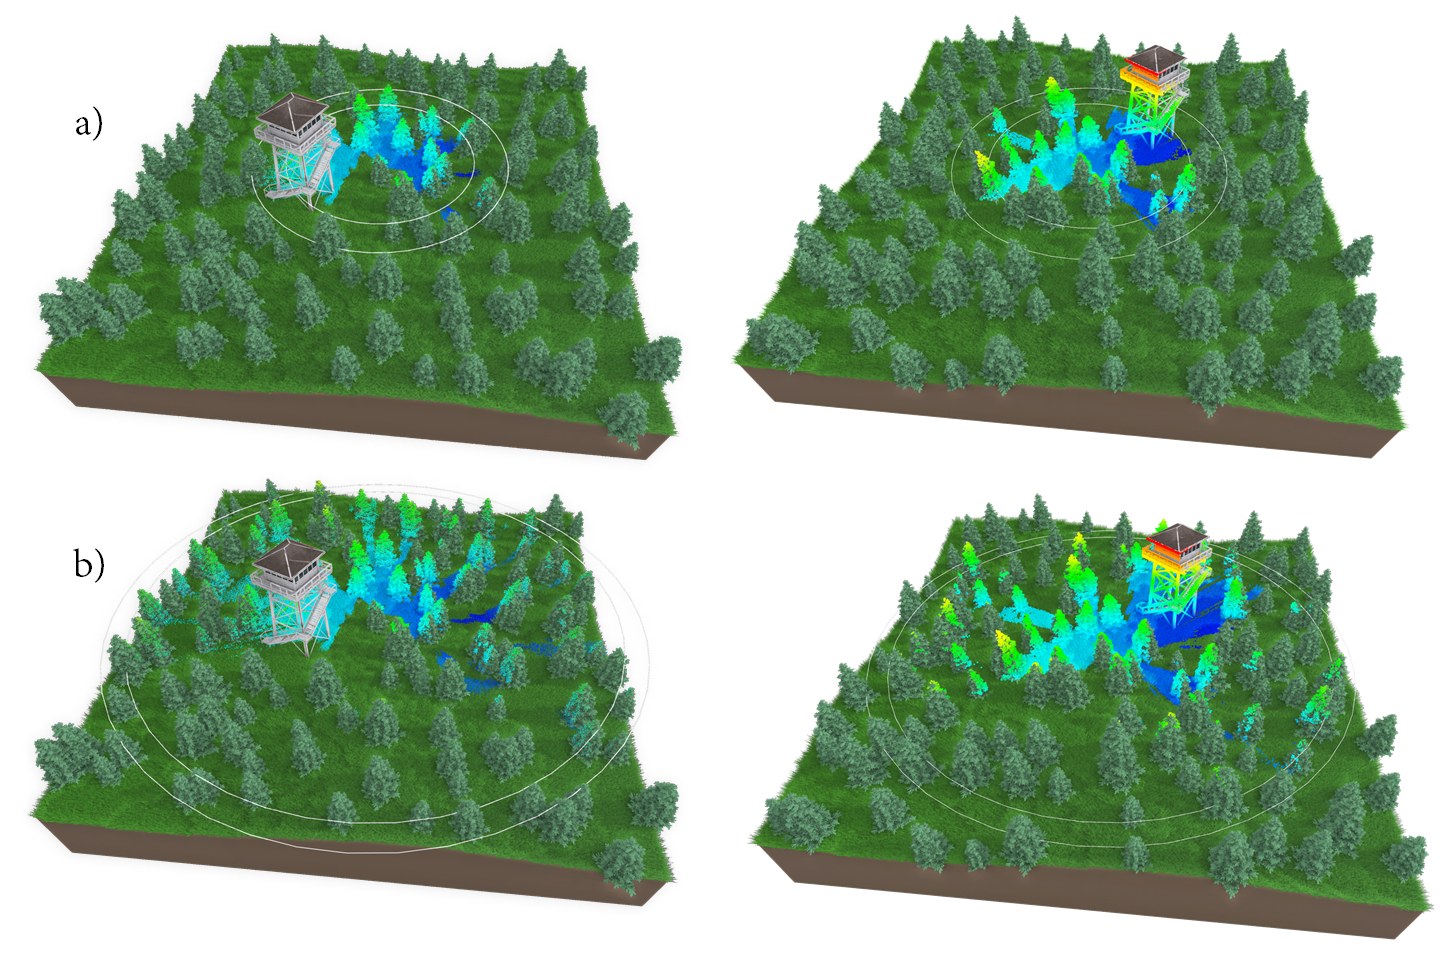
\includegraphics[width=\linewidth]{figs/lidar_simulation/tls_maximum_range.png}
	\caption{Scanning with very limited range, a), and with a larger range, b).}
	\label{fig:tls_maximum_range}
\end{figure}

\subsubsection{'Time-walk' effect}

This effect is simulated by translating returns according to three factors: the distance to the sensor's receiver and the indices that identify 1) the intersected surface and 2) a single collision in a unique way. Hence, index-related factors, $\delta_{\textit{object}}$ and $\delta_{\textit{return}}$ are intended to distort the returns according to either \textit{object} or \textit{return}. $\delta_{\textit{surface}}$ distorts every intersection from a surface with the same factor, thus preserving the shape, whereas $\delta_{\textit{return}}$ changes every return individually. Still, the magnitude of these errors is mainly driven by the distance factor (Equation \ref{eq:shiny_surface_error}).
\begin{equation}
    \label{eq:shiny_surface_error}
    \varrho = e_{\textit{glossy}} \cdot (d \cdot \hat{r}_{d} k_{\textit{distance}} + \hat{r}_{d}(\delta_{\textit{surface}}k_{\textit{surface}} + \delta_{\textit{collision}}k_{\textit{collision}})) 
\end{equation}
where $k_{\textit{distance}}$, $k_{\textit{surface}}$ and $k_{\textit{collision}}$ are constant values that control the magnitude of every equation term, $\textit{glossy}$ is a Boolean value that determines if such error is applied, and $d$ is the distance from the sensor to the intersection. Figure \ref{fig:shiny_surface_error} shows the translation applied to highly reflective objects if the \acrshort{lidar}'s emitter is close to the affected surfaces.

\begin{figure}[ht]
	\centering
	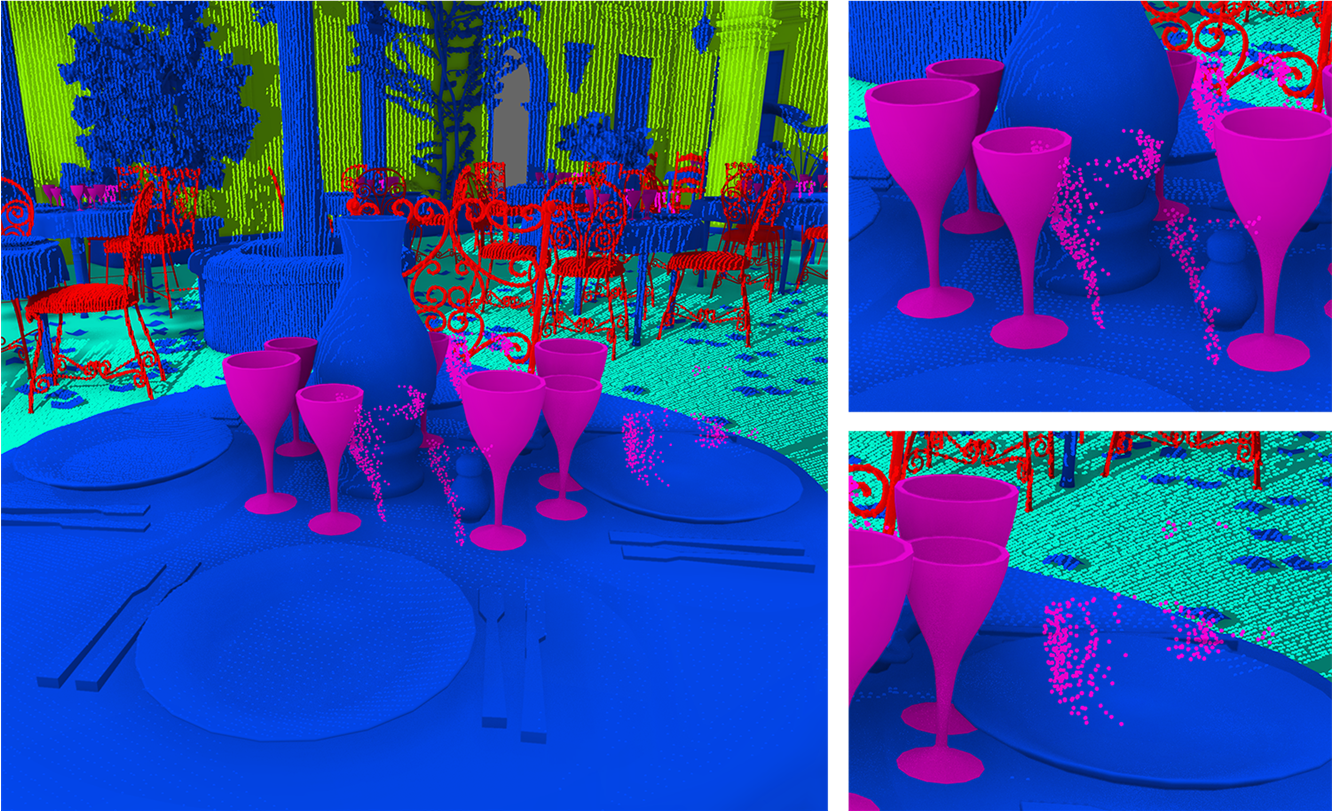
\includegraphics[width=\linewidth]{figs/lidar_simulation/glossy_time_walk.png}
	\caption{'Time-walk' effect simulated on glass surfaces rendered according to their semantic labels. }
	\label{fig:shiny_surface_error}
\end{figure}

\subsubsection{Slope derived errors}

Points are also distorted on steep surfaces according to the airborne flight altitude (vertical error) and the slope (horizontal error). The former is calculated as $\frac{h}{10^3}$ \si{\meter}, with $h$ being the airborne platform altitude \cite{hodgson_accuracy_2004}. The altitude-based error depends on the surface slope and flight altitude \cite{baltsavias_comparison_1999} as expressed in Equation \ref{eq:soil_induced_error}.
\begin{gather}
    \label{eq:soil_induced_error}
    \begin{aligned}
        \varrho = e_{\textit{terrain}} \cdot (&\delta_{h} k_{\textit{height}_{h}} h 
        \left[\delta_{x}, 0, \delta_{z}\right]^\intercal\\
        &+ \delta_{v} (k_{\textit{height}_{v}} h + k_{\alpha} \alpha)
        \left[0, 1, 0\right]^\intercal)
    \end{aligned}
\end{gather}
provided that $h$ is the flight altitude, $k_{\textit{height}_{v}}$, $k_{\textit{height}_{h}}$,  $k_{\alpha}$ weight the flight altitude and slope angle for the horizontal and vertical errors, and $\delta$ are random values in $[0, 1]$. Figure \ref{fig:terrain_induced_errors} shows the outcome of this distortion. All these errors can be omitted by weighting them as zero.

\begin{figure}
    \centering
    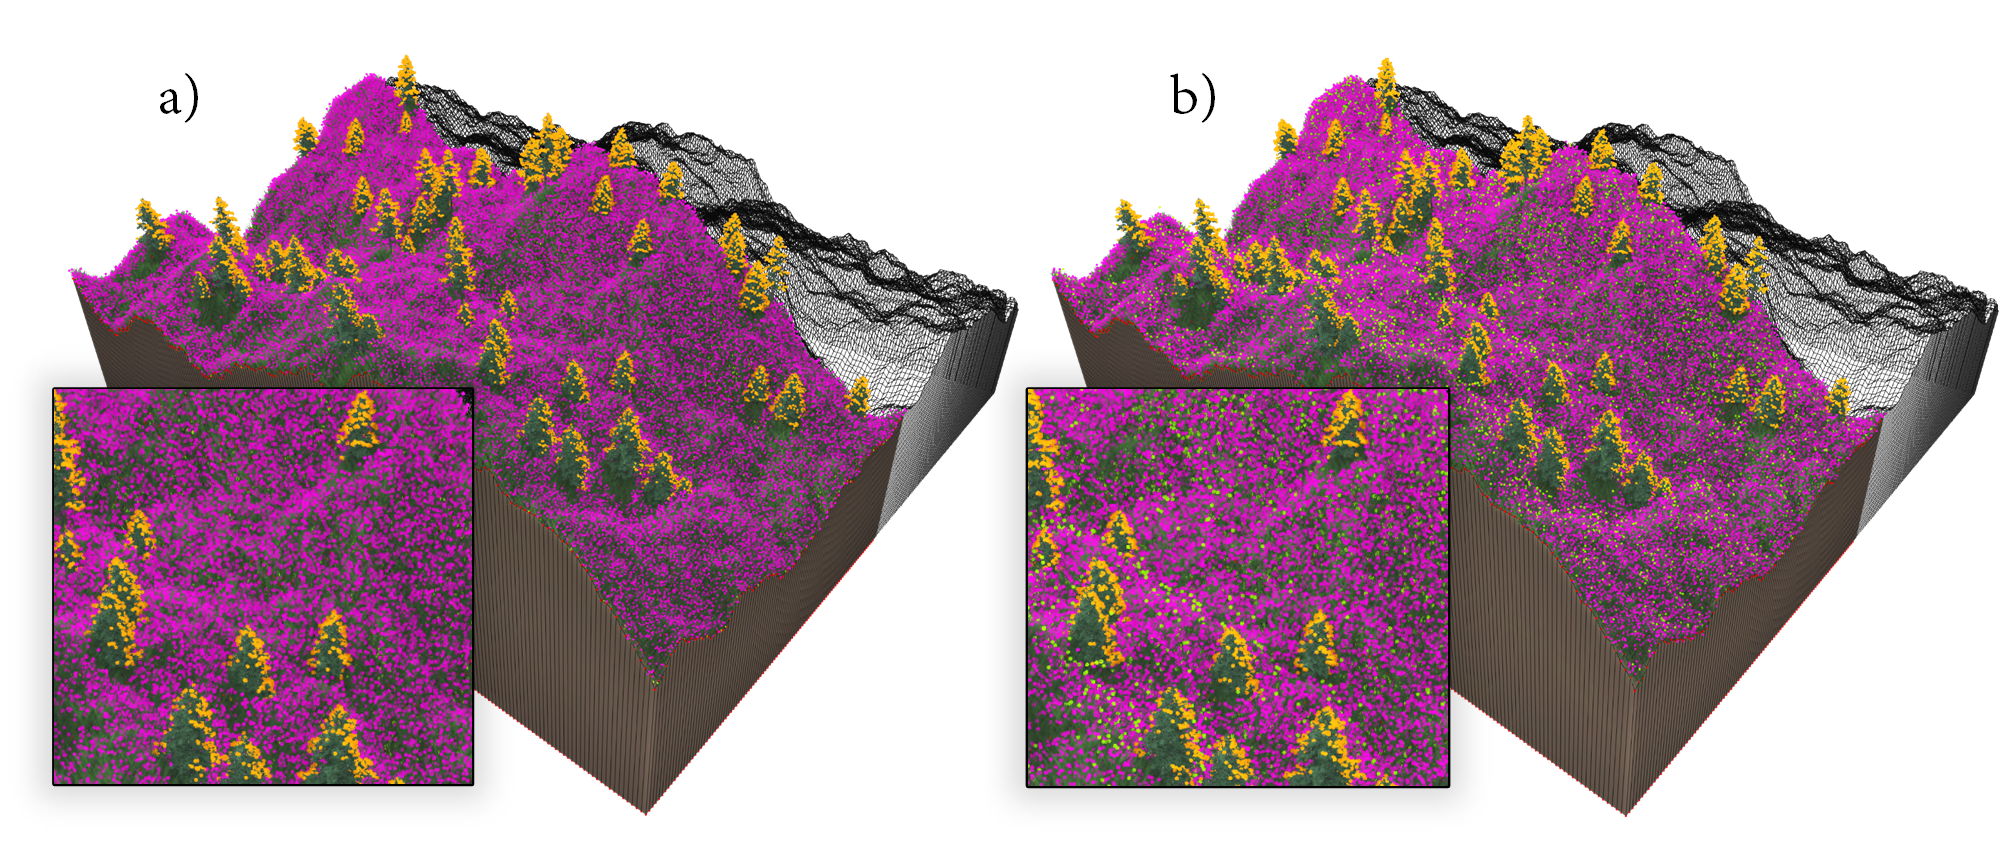
\includegraphics[width=\linewidth]{figs/lidar_simulation/terrain_induced_errors.png}
	\caption{Terrain-induced errors for a procedural environment. a) depicts an environment scanned without slope-based errors, whereas b) simulates such errors, thus making these points visible in the foreground. }
	\label{fig:terrain_induced_errors}
\end{figure}

\subsubsection{Bathymetric \acrshort{lidar}}

This kind of sensor presents some relevant changes with respect to the topographic \acrshort{lidar}. Bathymetric \acrshort{lidar} is able to detect surfaces underwater and yet propagates causing new returns. The ray's origin is always updated as $r_{o} = p + \epsilon$, whereas the ray's direction after colliding is computed from the refraction vector for the incident $\hat{r}_{d}$, the surface normal, $\hat{n}$, and the ratio of refractive indices, $r_{i}$. In addition, $r_{i}$ is given by the refractive index of the substance where the ray propagates, $\eta_{1}$, as well as the index of refraction from the substance of the intersected material, $\eta_{2}$. Moreover, $\eta_{2}$ depends on the wavelength of the \acrshort{lidar} sensor, and therefore, the material description must include the refractivity over different wavelengths.

\subsubsection{Return losses}

The return loss over glossy surfaces is driven by an exponential function, $g(k_{s})$, the coefficients $a, b, c, p$, a threshold $\textit{t}$ and the material's roughness, $k_s$, as shown in Equation \ref{eq:return_loss}. Hence, returns from glossy surfaces whose specular factor is above $\textit{t}$ are discarded whether the value retrieved from a random distribution is smaller than $g(k_{s})$. Accordingly, surfaces with lower reflectivity are less likely to cause return losses. Thus, it is possible to partially or entirely discard water returns with a step-function as the one depicted in Figure \ref{fig:glossy_loss}. 
\begin{gather}
    \label{eq:return_loss}
    g(k_{s}) = \begin{aligned}
        \begin{cases}
            c + a (k_{s} + b) ^ {p} &k_{s} > \textit{t}\\
            c &k_{s} \leq \textit{t}\\
        \end{cases}
    \end{aligned}
\end{gather}
where $c$ allows introducing some randomness even for diffuse materials. However, $c$ is defined as zero by default.

\begin{figure}
	\centering
	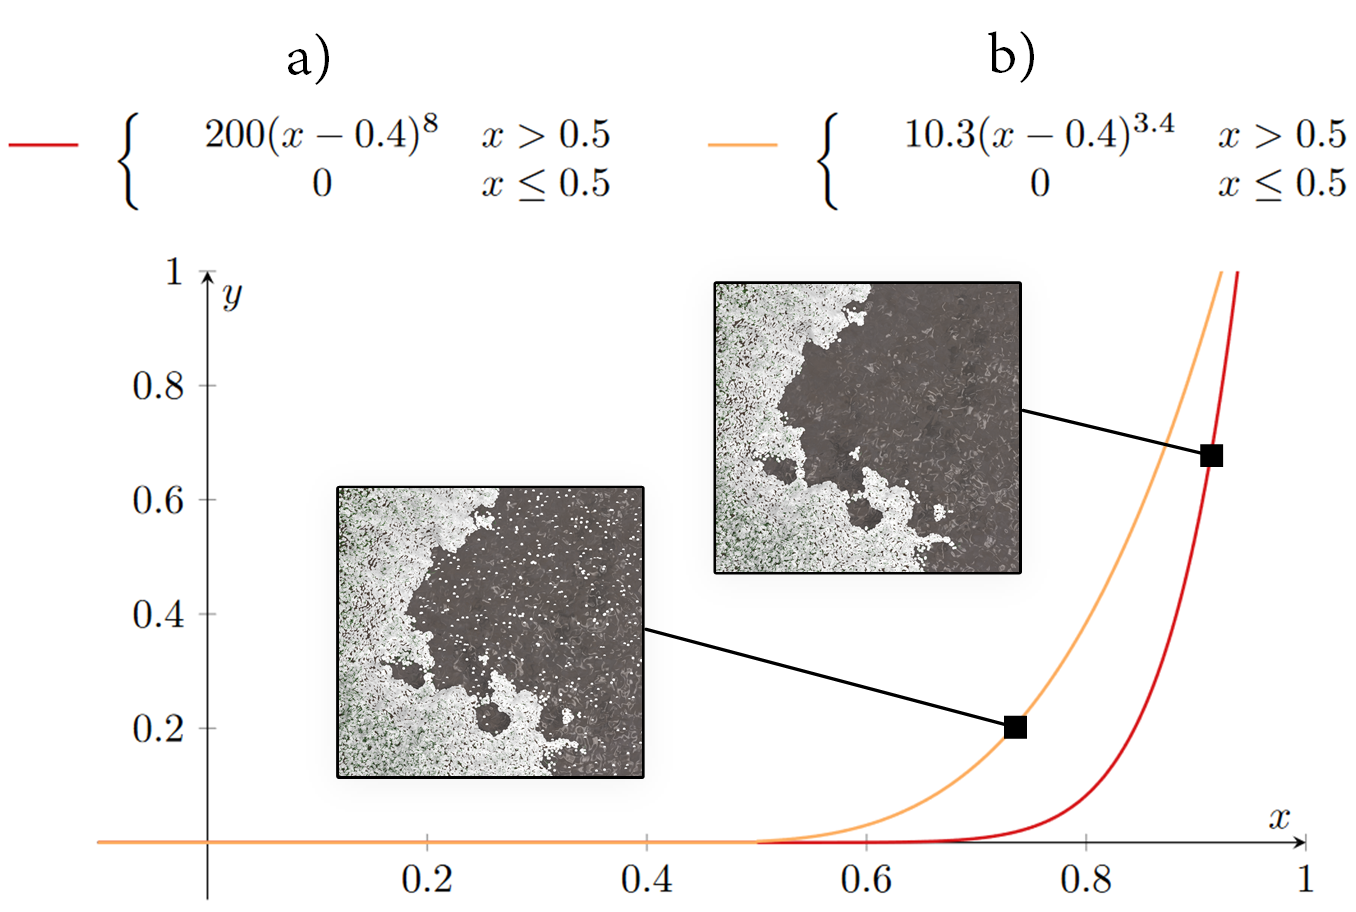
\includegraphics[width=.75\linewidth]{figs/lidar_simulation/glossy_loss.png}
	\caption{a) A loss function that slightly tolerates surfaces as glossy as water, and b) another loss function that discards every return from glossy surfaces. }
	\label{fig:glossy_loss}
\end{figure}

\subsubsection{Intensity computation}

This stage simulates radiometric information acquired by the virtual \acrshort{lidar}, which will be the matter of the following chapter. Note that radiometric data may also be relevant for \acrshort{dl} networks and therefore should be accurately modelled. The unitless returned intensity values are equally influenced by the surface material and the \acrshort{lidar} specifications, including the operating wavelength. The formulae describing the received optical power were already explained in Chapter \ref{sec:fundamentals_rs}, and therefore, we refer the reader to this section for further insight into the involved parameters. 

\begin{marginfigure}[.3cm]
	\centering
	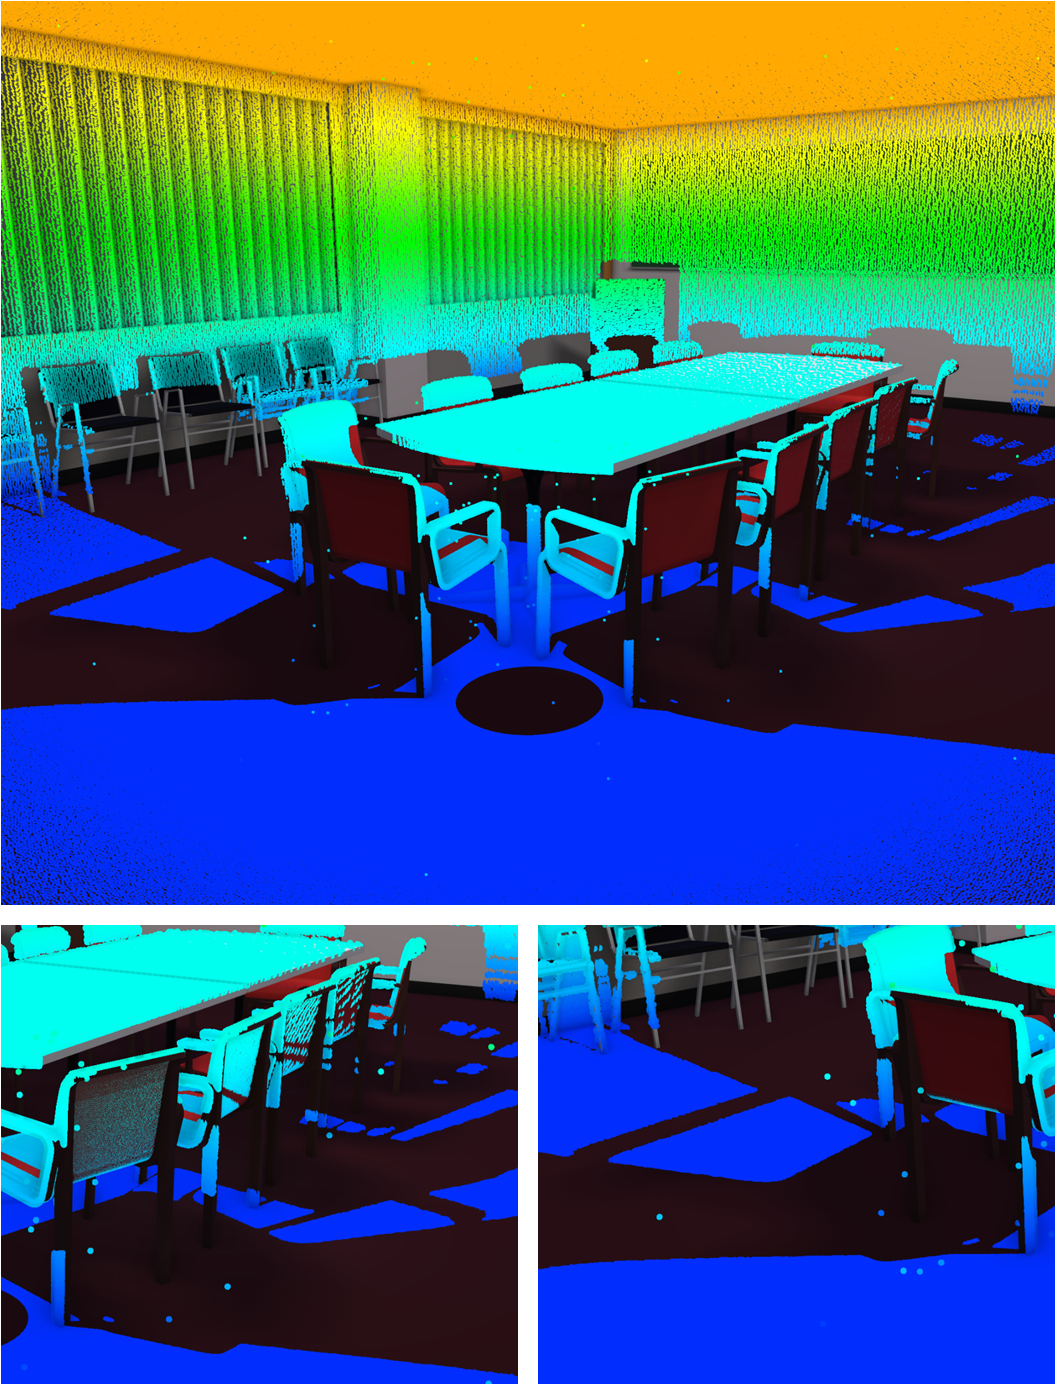
\includegraphics[width=\linewidth]{figs/lidar_simulation/outliers.png}
	\caption{Outliers in a \acrshort{tls} simulation, with $h \gets 0.95$.}
	\label{fig:lidar_outliers}
\end{marginfigure}

\subsubsection{Simulating outliers}

Outlier points are included to simulate errors caused by atmospheric particles such as dust or steam \cite{boehler_investigating_2018}. To this end, a variable amount ($t_{\textit{outlier}} \in [0, 1]$) of returns is translated along the ray's direction with a magnitude of $t \in [0, 1]$, which is modelled with a pseudo-random generation. In this case, the distribution from which noise is retrieved is particularly relevant to emulate the spatial distribution of outliers. The value $t$ refers to the parametric value in $p = r_o + r_d * t$. Figure \ref{fig:lidar_outliers} shows some outliers simulated at the Conference scenario.

\subsubsection{Update of return numbers}

Pulses are updated once all the rays are terminated or achieve the maximum number of returns. Returns are then changed to save the overall number of collisions per pulse. The return number provides valuable information since it helps to compute a factor $k_{\tau}$ defined as $\frac{\tau}{n_{\tau}}$, i.e., the return number, $\tau$ divided by the overall number of returns. Returns obtained in later iterations are more likely to belong to the ground; however, filtering by $\tau$ does not help to retrieve every ground point and filter out the rest. Instead, the last return of every pulse satisfies that $k_{\tau} > 1 - \epsilon$, and these are more appropriate to filter out vegetation and render only points close to the ground. For example, \acrshort{lidar} technology has been widely adopted in archaeology to detect remains which are not visible (either buried or occluded by the canopy) using the \acrshort{dsm} reconstructed with points that belong to the ground. 

\begin{figure}[ht]
	\centering
	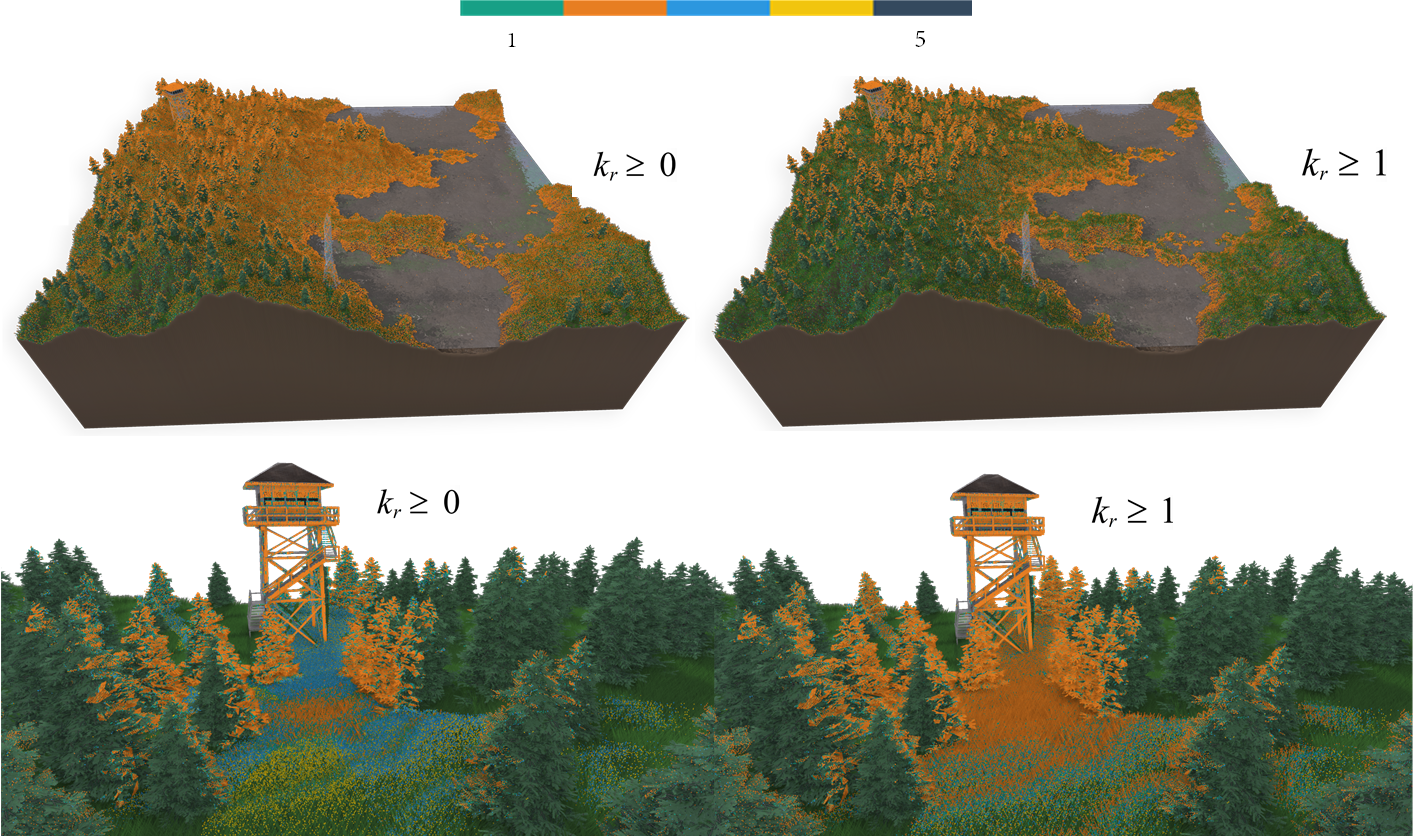
\includegraphics[width=1\linewidth]{figs/lidar_simulation/tls_multiple_returns.png}
	\caption{\acrshort{als} and \acrshort{tls} simulations over a procedural environment. First, the complete point cloud is rendered ($k_{r} \geq 0$), whereas the second image renders only the last return of each pulse.}
	\label{fig:multiple_returns}
\end{figure}

Figure \ref{fig:multiple_returns} depicts two different point clouds filtered by means of $k_{\tau}$ to visualize the last return of each pulse. The forest canopy was significantly dense and many pulses did not penetrate vegetation, whereas low vegetation was easily avoided. Accordingly, it shows a much less dense point cloud at ground level when $k_{\tau} \geq 1$ by filtering out vegetation.

\section{Results and discussion}

The proposed \acrshort{lidar} simulator has been tested against static and procedural scenes with high polygonal complexity (from 4.5M triangles to 11M). Also, the performance was checked by considering both response time and resulting point clouds. Therefore, the \acrshort{gpu}- and \acrshort{cpu}-based approaches were compared. Then, the proposed simulation was compared against several state-of-the-art \acrshort{lidar} solutions by addressing both quantitative metrics, such as the facilities to generate dense semantic datasets, and qualitative factors, such as the similarity of the point clouds with respect to real-world \acrshort{lidar} scans. 

Measurements were performed using a PC with Intel Core i9-9900 3.1 GHz, 48 GB RAM, RTX 2080 Ti \acrshort{gpu} with 11 GB RAM (Turing architecture). The proposed methodology was implemented in C++ along with \acrshort{opengl}. Massively parallel processes were either implemented in the \acrshort{gpu}, either using \acrshort{glsl} and general-purpose compute shaders or \acrshort{cpu} multi-threading with \acrshort{openmp}. 

\subsection{\acrshort{lidar} response time}

A comparison of the \acrshort{gpu}-based solution against its analogous multi-core \acrshort{cpu} approach will be first carried out to show the efficiency of the proposed simulation. Synchronism was established among the pipeline stages to await the end of different \acrshort{gpu} calls, thus allowing us to measure the stage-wise latency in the \acrshort{gpu}. Note that the response time from ray instancing is shared for the same \acrshort{lidar} configuration, whereas the rest of the stages are very influenced by the scenario. Figure \ref{fig:lidar_response_time_global} summarizes the results obtained for \acrshort{tls} and \acrshort{als} surveys, using scenes with an increasing number of polygons: Suburb (4.1M), San Miguel (4.5M), City (10.1M) and Forest (11M). Simulations with multiple returns were bounded to five returns. Further insight into the results is provided in Table \ref{table:lidar_response_time}.

\begin{figure*} [ht]
	\centering
	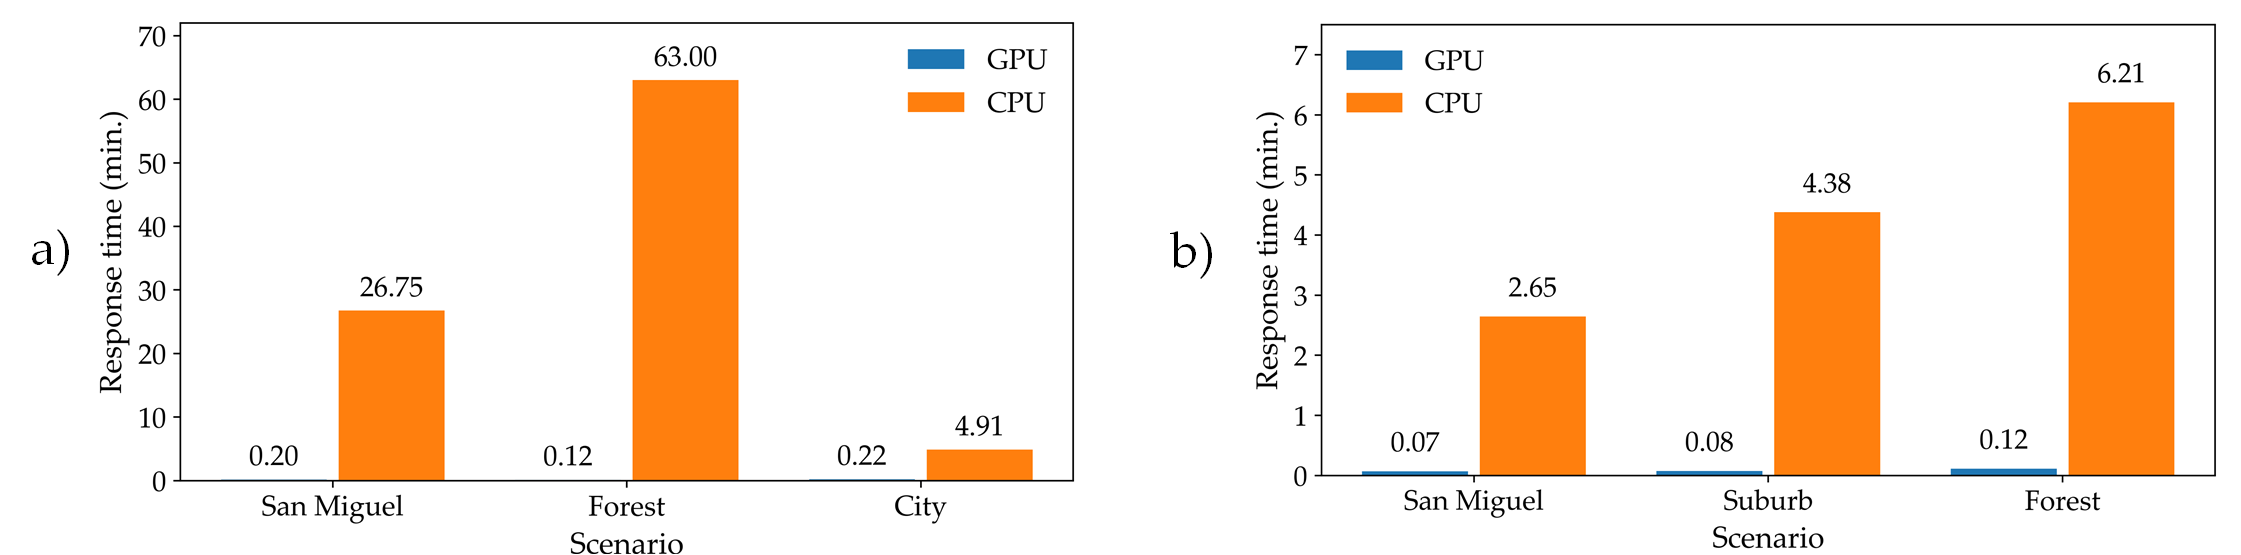
\includegraphics[width=\linewidth]{figs/lidar_simulation/response_time.png}
	\caption{Comparison of response time between the \acrshort{gpu} and multi-core \acrshort{cpu} approaches using a) \acrshort{tls} and b) \acrshort{als} with 10M pulses, 10 rays per pulse and multiple returns. }
	\label{fig:lidar_response_time_global}
\end{figure*}

\textbf{Ray build time}. \acrshort{tls} beams were straightforwardly computed, and thus the instancing phase shows lower latency. On the other hand, \acrshort{als} beams require a larger number of parameters and processing involving angles and the platform path. The response time for 10M pulses grows linearly with respect to 5M. Despite \acrshort{cpu}-based ray-instancing not being as time-consuming as the \acrshort{lidar} core, the speedup ranged from 90.9\% (\acrshort{als}, 10M pulses) to 99.12\% (\acrshort{tls}, 10M pulses).

\textbf{\acrshort{lidar} behaviour}. The \acrshort{tof} solver operates for every batch of rays, with the batch dimensionality being limited by the maximum allocatable memory for an \acrshort{ssbo}. In this stage, the response time is also proved to grow linearly according to the number of pulses. However, \acrshort{als} surveys show lower latency both in \acrshort{cpu} and \acrshort{gpu} since the scene geometry is less dense in the vertical axis, and thus, the \acrshort{bvh} clusters are rapidly discarded. Although \acrshort{ssbo}s are very limited in size, reducing it beyond the limit queried from \acrshort{opengl} helped to reduce the latency, apparently from a lower \acrshort{gpu} overload. This factor was also parameterized to be tuned during these tests.

Although \acrshort{tls} scans are notably slower, the reported speedup with respect to the sequential approach is impressive: San Miguel (99.27\%), Forest (99.81\%) and City (95.06\%). \acrshort{als} scans, on the other hand, achieve the following speedups: San Miguel (98.62\%), Forest (98.71\%) and Suburb (99.15\%).

\begin{figure*}
    \centering
    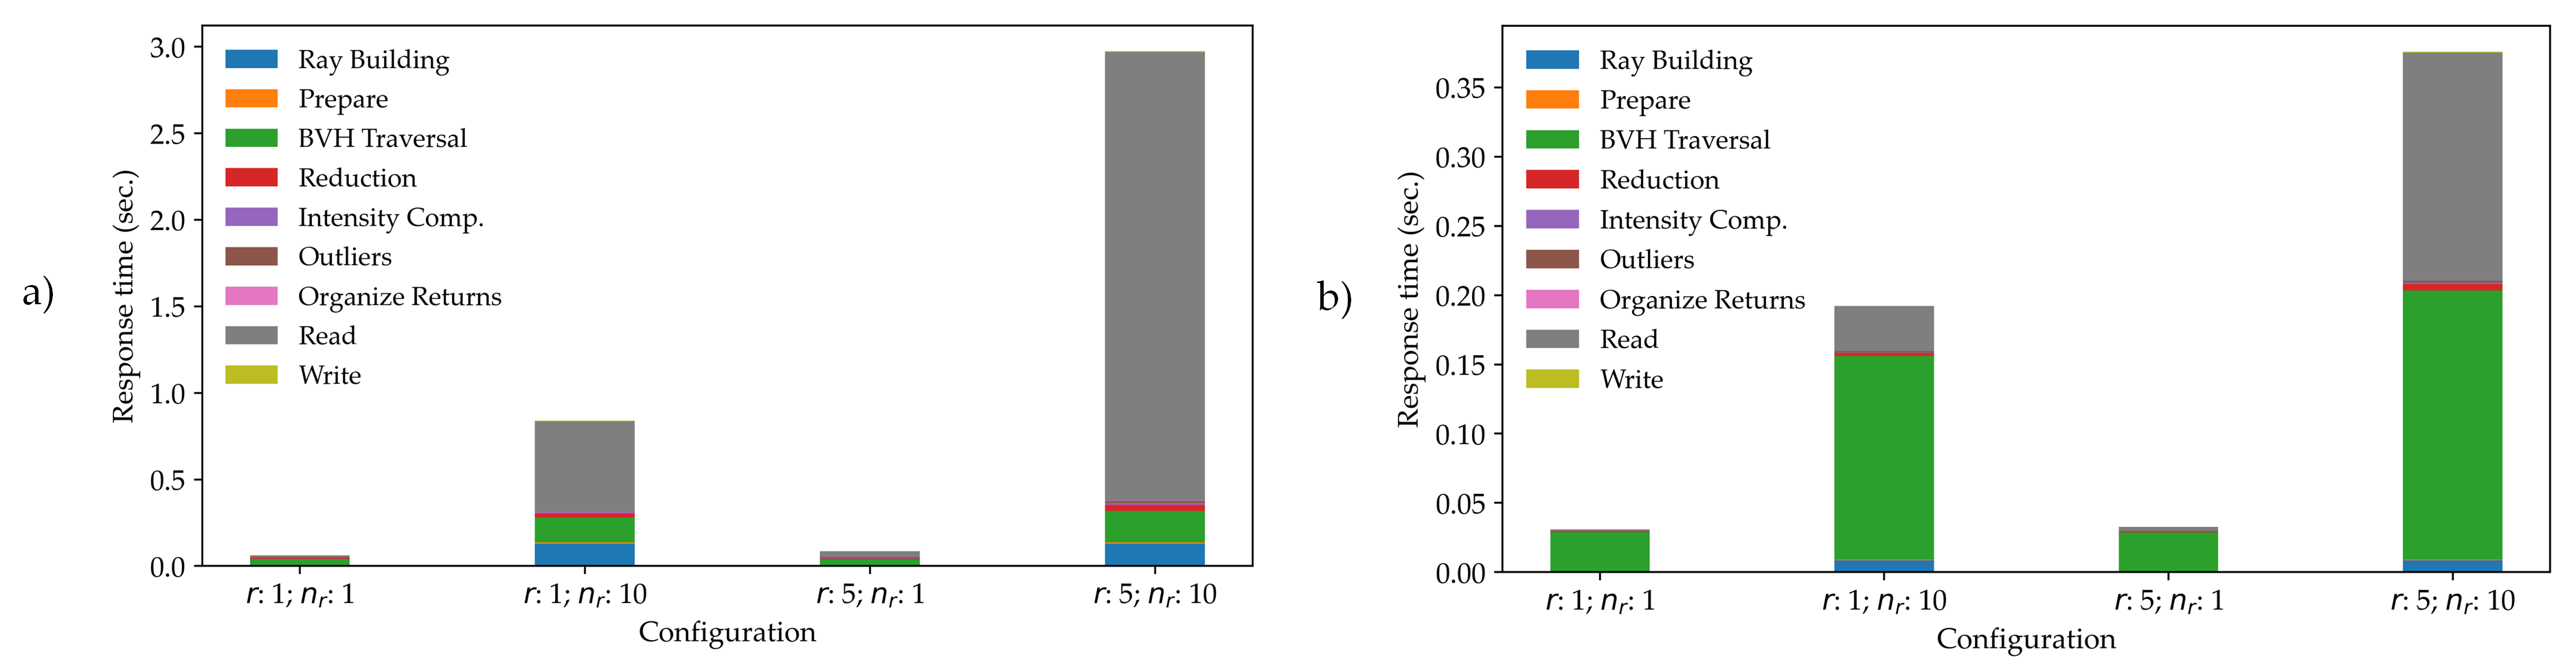
\includegraphics[width=\linewidth]{figs/lidar_simulation/lidar_response_time_stage.png}
	\caption{Absolute (left) and relative (right) response time of \acrshort{lidar} stages. a) The first chart row compares the performance of \acrshort{tls} in a procedural forest, using a different number of allowed returns ($r$) and rays within a pulse ($n_r$). Similarly to \acrshort{tls}, the second chart row presents the results for an \acrshort{als} sensor.}
	\label{fig:lidar_response_time_chart}
\end{figure*}

\textbf{Stage occupancy}. Besides the overall response time, the individual latency of every stage was also measured. To this end, stages were explicitly synchronized in the \acrshort{cpu} instead of allowing \acrshort{opengl} to handle parallelism and memory access. Figure \ref{fig:lidar_response_time_chart} shows the relative latency for high-performance tests using environments from lower (5M) to higher complexity (10M) scanned with 5M pulses. Apart from the phases depicted in Figure \ref{fig:lidar_workflow}, reading transfers from \acrshort{gpu} to \acrshort{cpu} were also included as they were required to perform further processing in the \acrshort{cpu} and store the results as part of the simulated point cloud. Instead of constructing the whole ray buffer at once, rays were iteratively constructed to avoid \acrshort{cpu} and \acrshort{gpu} data transfers.

As reported, transferring collisions to the \acrshort{cpu} takes a substantial portion of time, whereas \acrshort{bvh} traversals are notably more time-consuming for highly populated environments. However, traversing a scene is significantly slower for \acrshort{tls} scans as they cannot discard clusters as rapidly. The reduction stage is also relevant in this chart due to the operations performed pulse-wise; note that in this stage, every ray within a pulse is processed by the same thread. 

\newcommand{\datasetImageHeight}{-.06\totalheight}
\newcommand{\datasetImageSize}{1.4cm}
\newcommand{\lidarCoreLabel}{ToF Solver}

\renewcommand{\arraystretch}{1.2}
\begin{table*}[hb]
    \footnotesize
    \centering
    \caption{Comparison of \acrshort{cpu} and \acrshort{gpu} response time for \acrshort{tls} and \acrshort{als} scans. The results were obtained using static and procedural scenes with a significant number of triangles.}
    \label{table:lidar_response_time}
    \begin{tabular}{c|c|c|llll}
    \toprule
    \multicolumn{7}{c}{\textbf{Terrestrial \acrshort{lidar}}}\\
    \cmidrule{1-7}
    \multicolumn{3}{c}{\textbf{Configuration}} & &
    \raisebox{\datasetImageHeight}{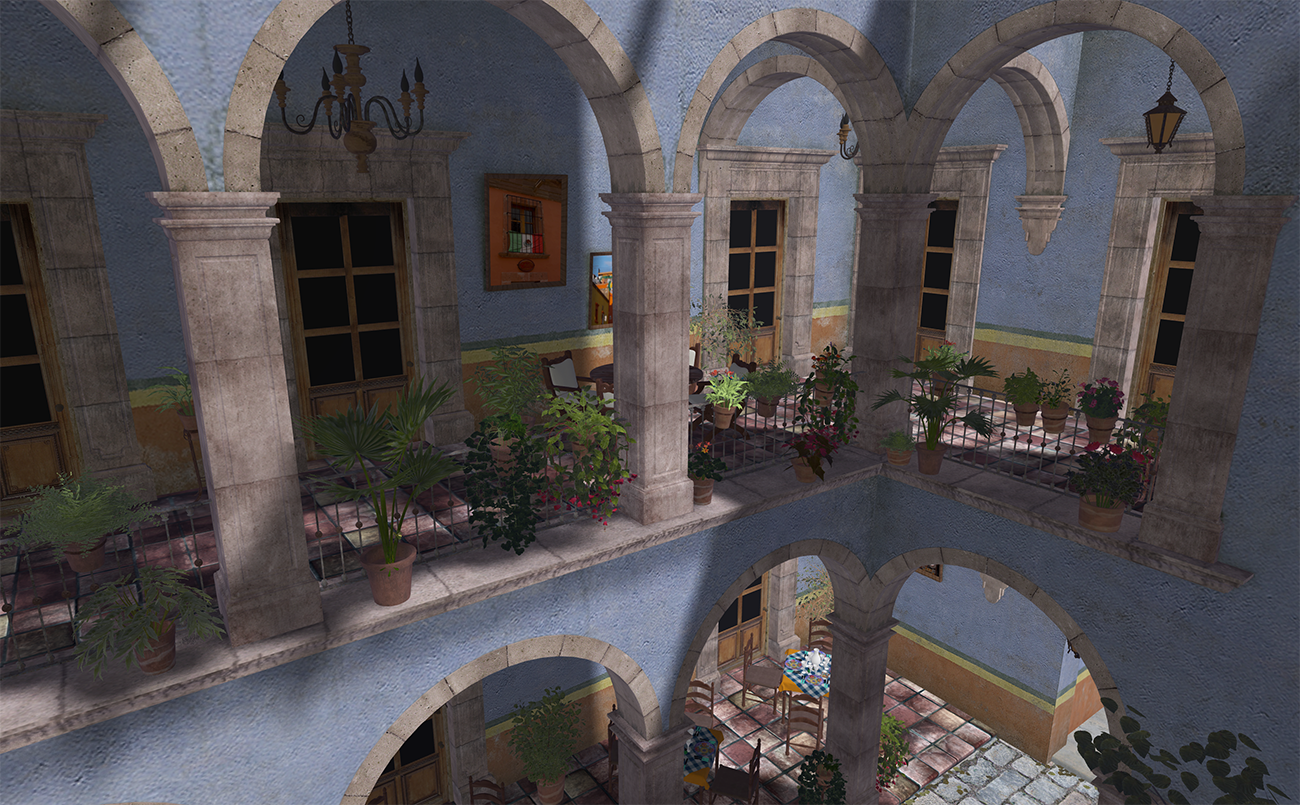
\includegraphics[width=\datasetImageSize]{figs/datasets/san_miguel.png}} \hspace{1mm}
    \shortstack{San Miguel\\ \#triangles\\ 5.6M } & \raisebox{\datasetImageHeight}{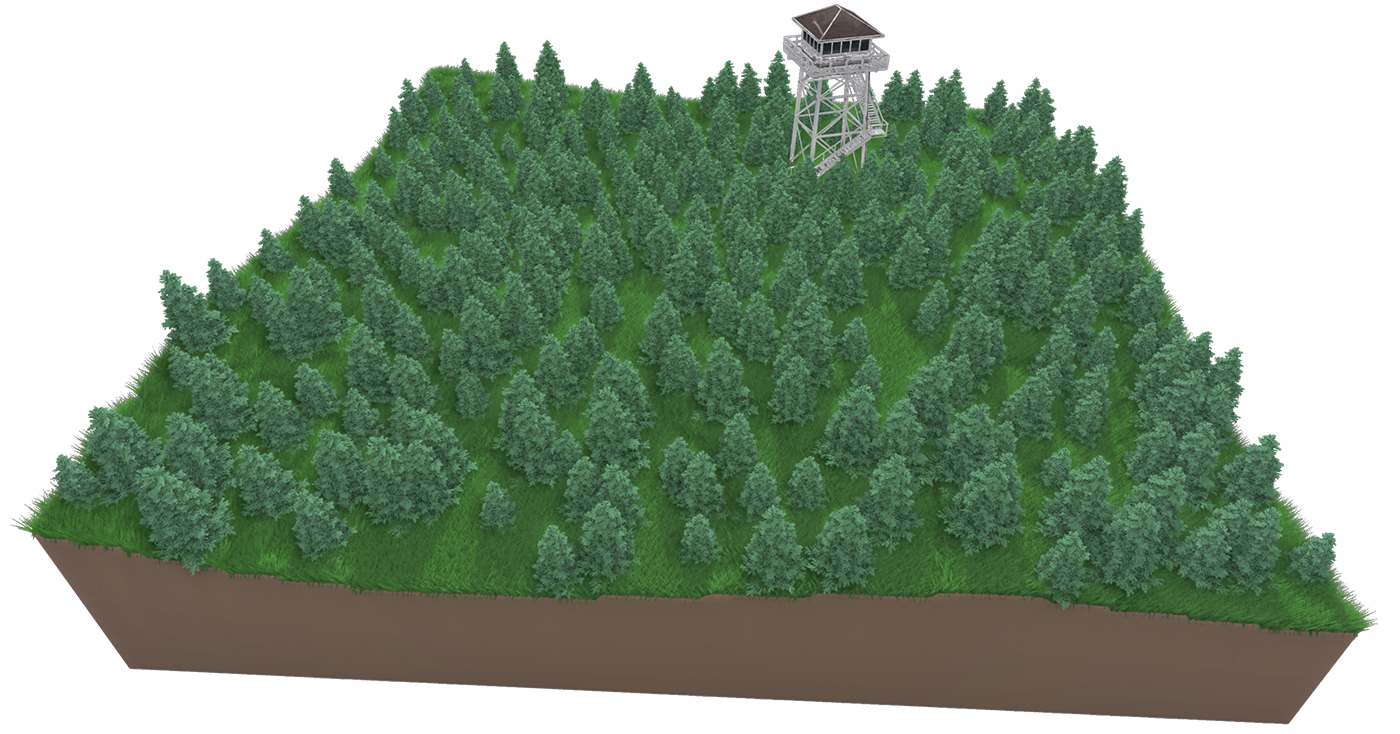
\includegraphics[width=\datasetImageSize]{figs/datasets/tls_forest.png}} \hspace{1mm}
    \shortstack{Forest\\ \#triangles\\ 11M } &
    \raisebox{\datasetImageHeight}{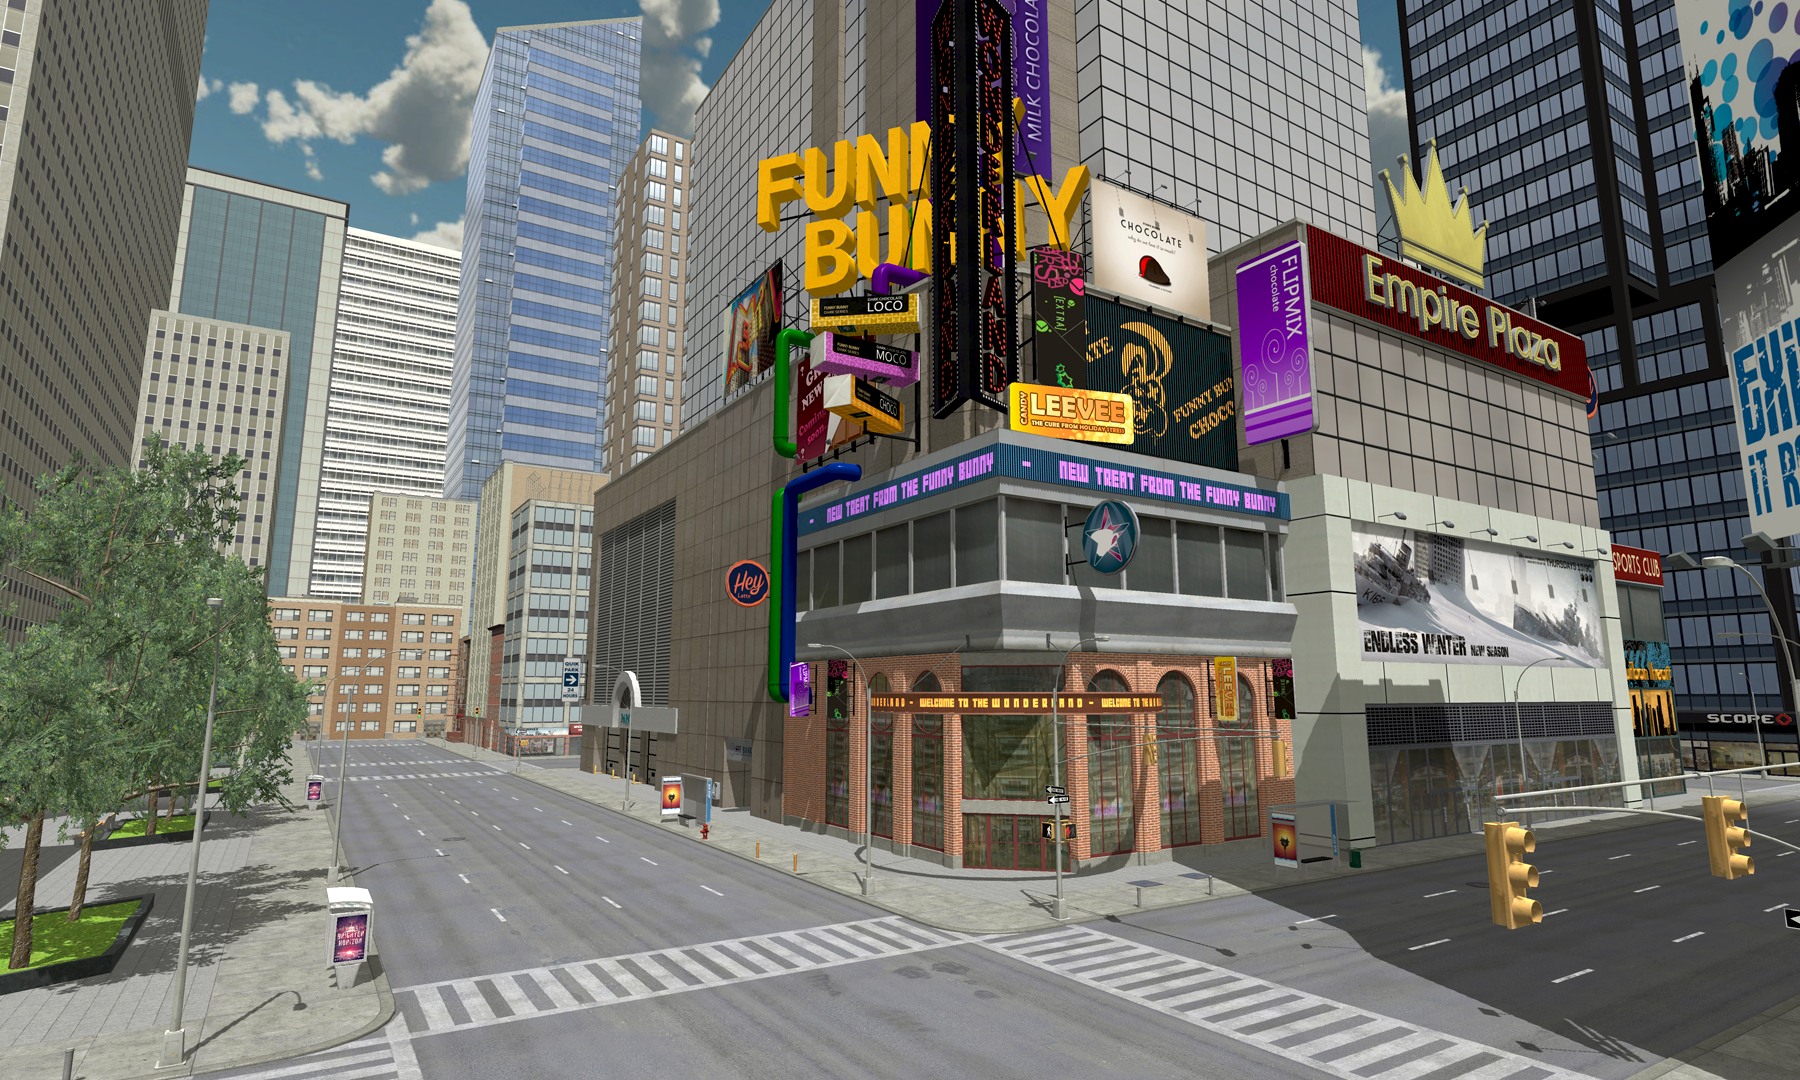
\includegraphics[width=\datasetImageSize]{figs/datasets/mcp.png}} \hspace{1mm}
    \shortstack{City\\ \#triangles\\ 10.1M }\\
    \cmidrule{1-7}
    \textbf{$n_{p}$} & Method & \textbf{$n_{r}$} & Ray inst. & \lidarCoreLabel & \lidarCoreLabel & \lidarCoreLabel\\
    \cmidrule{1-7}
    \multicolumn{7}{c}{Single return}\\
    \cmidrule{1-7}
    \multirow{2}{*}{5M} & \textbf{\acrshort{gpu}} & \multirow{2}{*}{10} & 
    \textbf{0.141s} & \textbf{2.747s} & \textbf{0.755s} & \textbf{3.664s}\\ 
    & \acrshort{cpu} & & 
    15.601s & 193.790s & 1,854.337 & 128.900s\\
    \cmidrule{1-7}
    \multirow{2}{*}{10M} & \textbf{\acrshort{gpu}} & \multirow{2}{*}{10} & 
    \textbf{0,279s} & \textbf{5.254s} & \textbf{1.510s} & \textbf{7.745s}\\ 
    & \acrshort{cpu} & & 
    31.740s & 1,571.758s & 3,743.797s & 261.091s\\
    \toprule
    \multicolumn{7}{c}{Multiple returns (5)}\\
    \cmidrule{1-7}
    \multirow{2}{*}{5M} & \textbf{\acrshort{gpu}} & \multirow{2}{*}{10} & 
    \textbf{0,141s} & \textbf{5.637s} & \textbf{3.323s} & \textbf{6.597s}\\ 
    & \acrshort{cpu} & & 
    15,601s & 194,533s & 1.900,348s & 129,725s\\
    \cmidrule{1-7}
    \multirow{2}{*}{10M} & \textbf{\acrshort{gpu}} & \multirow{2}{*}{10} & 
    \textbf{0.279s} & \textbf{11.481s} & \textbf{6.906s} & \textbf{12.949s}\\ 
    & \acrshort{cpu} & & 
    31.740s & 1,573.349s & 3,748.547s & 262.640s\\
    \cmidrule{1-7}
    \multicolumn{7}{c}{\textbf{Aerial \acrshort{lidar}}}\\
    \cmidrule{1-7}
    \multicolumn{3}{c|}{\textbf{Configuration}} & &
    \raisebox{\datasetImageHeight}{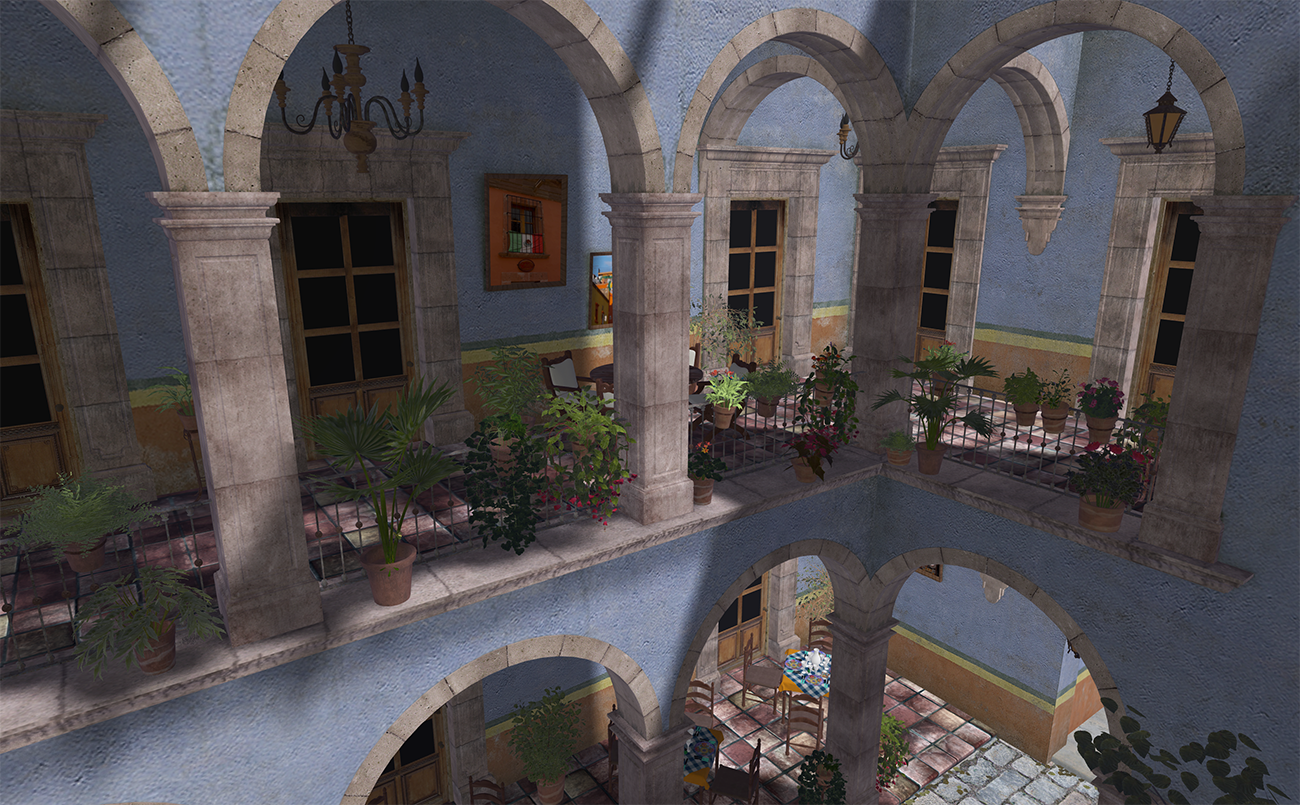
\includegraphics[width=\datasetImageSize]{figs/datasets/san_miguel.png}} \hspace{1mm}
    \shortstack{San Miguel\\ \#triangles\\ 5.6M } & \raisebox{\datasetImageHeight}{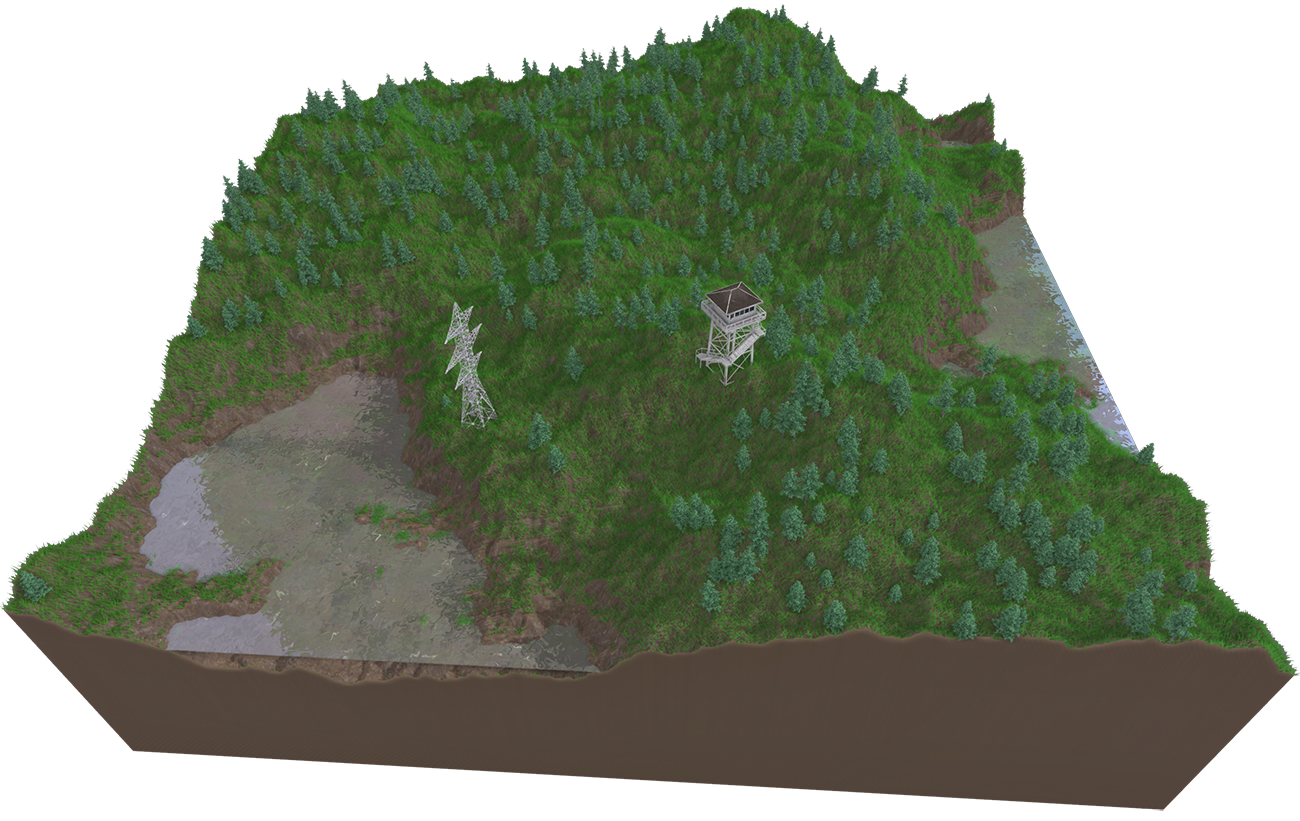
\includegraphics[width=\datasetImageSize]{figs/datasets/als_forest.png}} \hspace{1mm}
    \shortstack{Forest\\ \#triangles\\ 11M } &
    \raisebox{\datasetImageHeight}{\includegraphics[width=\datasetImageSize]{figs/datasets/suburb.png}} \hspace{1mm}
    \shortstack{Suburb\\ \#triangles\\ 4.1M }\\
    \cmidrule{1-7}
    \textbf{$n_{p}$} & Method & \textbf{$n_{r}$} & Ray inst. & \lidarCoreLabel & \lidarCoreLabel & \lidarCoreLabel\\
    \cmidrule{1-7}
    \multicolumn{7}{c}{Multiple returns (5)}\\
    \cmidrule{1-7}
    \multirow{2}{*}{5M} & \textbf{\acrshort{gpu}} & \multirow{2}{*}{10} & 
    \textbf{1.240s} & \textbf{0.923s} & \textbf{2.348s} & \textbf{0.995s}\\ 
    & \acrshort{cpu} & & 
    12.586s & 66.889s & 102.070s & 119.946s\\
    \cmidrule{1-7}
    \multirow{2}{*}{10M} & \textbf{\acrshort{gpu}} & \multirow{2}{*}{10} & 
    \textbf{2.510s} & \textbf{1.806s} & \textbf{4.4294s} & \textbf{1.996s}\\ 
    & \acrshort{cpu} & & 
    27.583s & 131.253s & 344.882s & 235.174s\\
    \bottomrule
    \end{tabular}
    \libertineNormal
\end{table*}
\renewcommand{\arraystretch}{1}

\subsection{Generation of synthetic datasets}

Another main objective of this work is to provide a framework for generating large semantic datasets. Thus, several tests were conducted to evaluate both the dimensionality and the number of labels in the collected datasets. Comparisons were established with previously cited work \cite{yue_lidar_2018, xiao_synlidar_2021, behley_towards_2021, pan_semanticposs_2020, caesar_nuscenes_2020}, either based on real or synthetic datasets, by taking into account the number of scans, the overall number of points, as well as the number of semantic annotations. To provide a fair evaluation, the tests were performed using the configuration of a Velodyne HDL-64E \cite{su_simulation_2019}, as proposed in most of the urban datasets in the literature \cite{behley_towards_2021, xiao_synlidar_2021, caesar_nuscenes_2020}. Aerial surveys are, on the other hand, not frequent in previous work. Accordingly, other simulations have been carried out using the configuration of an airborne DJI Zenmuse L1 sensor \cite{dji_zenmuse_2020}. Remark that some of the sensor parameters were not provided by the manufacturers, and therefore were adjusted to generate dense point clouds (Table \ref{table:test_sensor_parameters}). Also, the variable height of urban environments required solving the surveys with multiple scans at different altitudes.

\renewcommand{\arraystretch}{1.25}
\begin{table*}
    \centering
    \caption{Overview of outdoor \acrshort{lidar} datasets with semantic annotations, regarding their average size ($\textit{Points} / \textit{Scans}$) and number of classes (Labels).}
    \label{table:lidar_dataset_comparison}
    \centering
    \begin{tabular}{llllll}
    \hline
    \textbf{Dataset} & \textbf{Annotation} & \textbf{Number of scans} & \textbf{Average size} & \textbf{Labels} & \textbf{Synthetic}\\
    \midrule
    SynLiDAR \cite{xiao_synlidar_2021} & Point-wise & 198,396 & 98.197k points & 32 & \cmark \\
    GTA-LiDAR \cite{yue_lidar_2018} & Pixel-wise & 121,087 & - & 2 & \cmark \\
    Semantic3D \cite{hackel_semantic3d_2017} & Point-wise & 30 & \textbf{133.3M} points & 8 & \xmark \\
    SemanticKITTI \cite{behley_towards_2021} & Point-wise & 43,552 & 105.79k points & 25 & \xmark \\
    SemanticPOSS \cite{pan_semanticposs_2020} & Point-wise & 2,988 & 72.289k points & 14 & \xmark \\
    nuScenes \cite{caesar_nuscenes_2020} & Point-wise & 40,000 & 35k points & 32 & \xmark \\
    \midrule
    Ours & Point-wise & 488 & 622.95k points & \textbf{53} & \cmark \\
    \bottomrule
    \end{tabular}
\end{table*}

The results were collected by scanning two virtual urban scenes. The first has 32 semantic classes, whereas the second environment presents 45 semantic annotations. Furthermore, these scenes were populated with procedural pedestrians and vehicles. After scanning both environments, an average frame size of nearly 623k points was reported from 488 scans, either from \acrshort{tls} or \acrshort{als}, which greatly improves the current average size of synthetic \acrshort{lidar} simulators. Despite real-world datasets acquiring more dense point clouds, e.g., Semantic3D \cite{hackel_semantic3d_2017}, the main contribution of virtual scans is their low response time and efficiency both in acquiring data and annotating each point. Furthermore, the conducted tests were only performed over procedural environments generated with a single seed. Otherwise, a large number of differently populated environments could be modelled to further collect synthetic \acrshort{lidar} datasets.

Figure \ref{fig:lidar_urban_scan} illustrates the semantic labels of the input scenarios as well as the point clouds collected from \acrshort{tls} and \acrshort{als} scans, coloured with their height. The number of points annotated with different categories is depicted in Figure \ref{fig:semantic_histogram}, by reporting points returned from \acrshort{tls} and the fusion of both \acrshort{tls} and \acrshort{als} (Table \ref{table:lidar_dataset_comparison}). Despite the contribution of \acrshort{als} scans being relevant for augmenting the dataset labels, the weight on the bar chart is very reduced in comparison with \acrshort{tls} scans due to the lower number of pulses.

\begin{figure*}[ht]
    \centering
    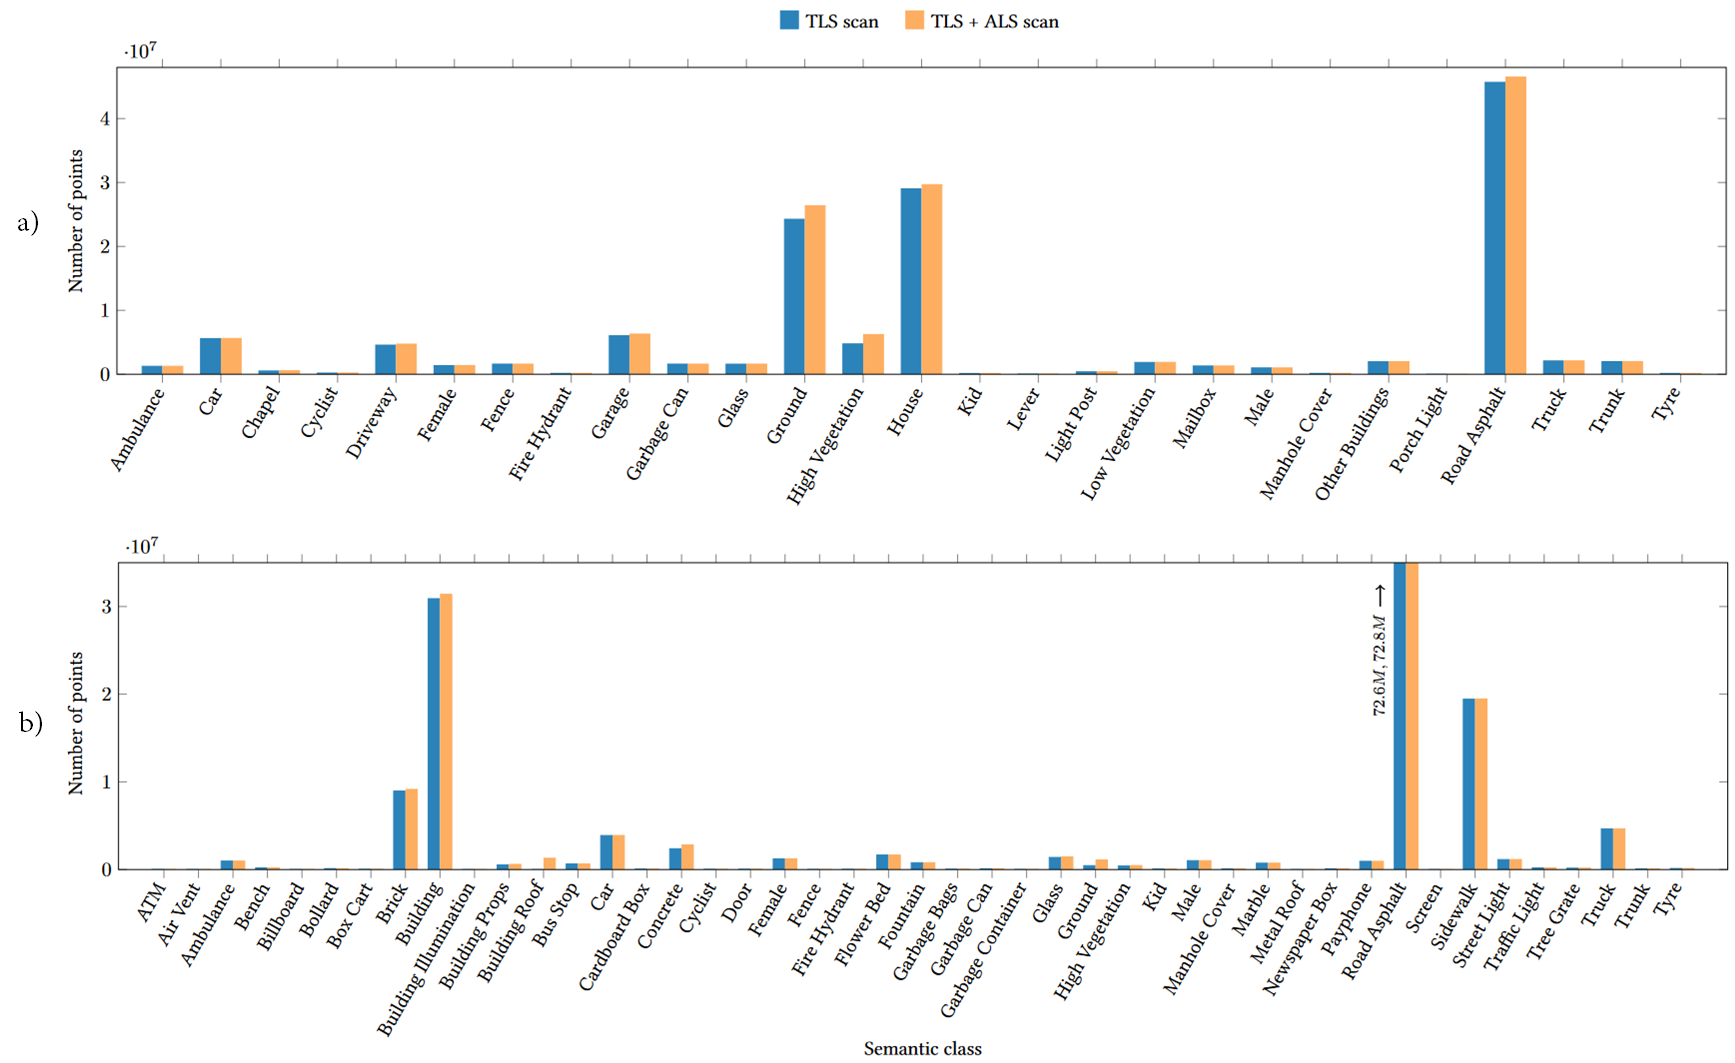
\includegraphics[width=\linewidth]{figs/lidar_simulation/bar_chart_annotations.png}
	\caption{Number of \acrshort{lidar} points per semantic label in two different urban environments. The first bar reports the results of \acrshort{tls} scans, whereas the second bar shows the results combining both \acrshort{als} and \acrshort{tls}. a) Distribution of 139M and 145M points for \acrshort{tls} and \acrshort{tls} + \acrshort{als} scans, respectively, whereas b) shows the profile generated by 165M and 170M points. }
	\label{fig:semantic_histogram}
\end{figure*}

\begin{figure*}[ht]
    \centering
    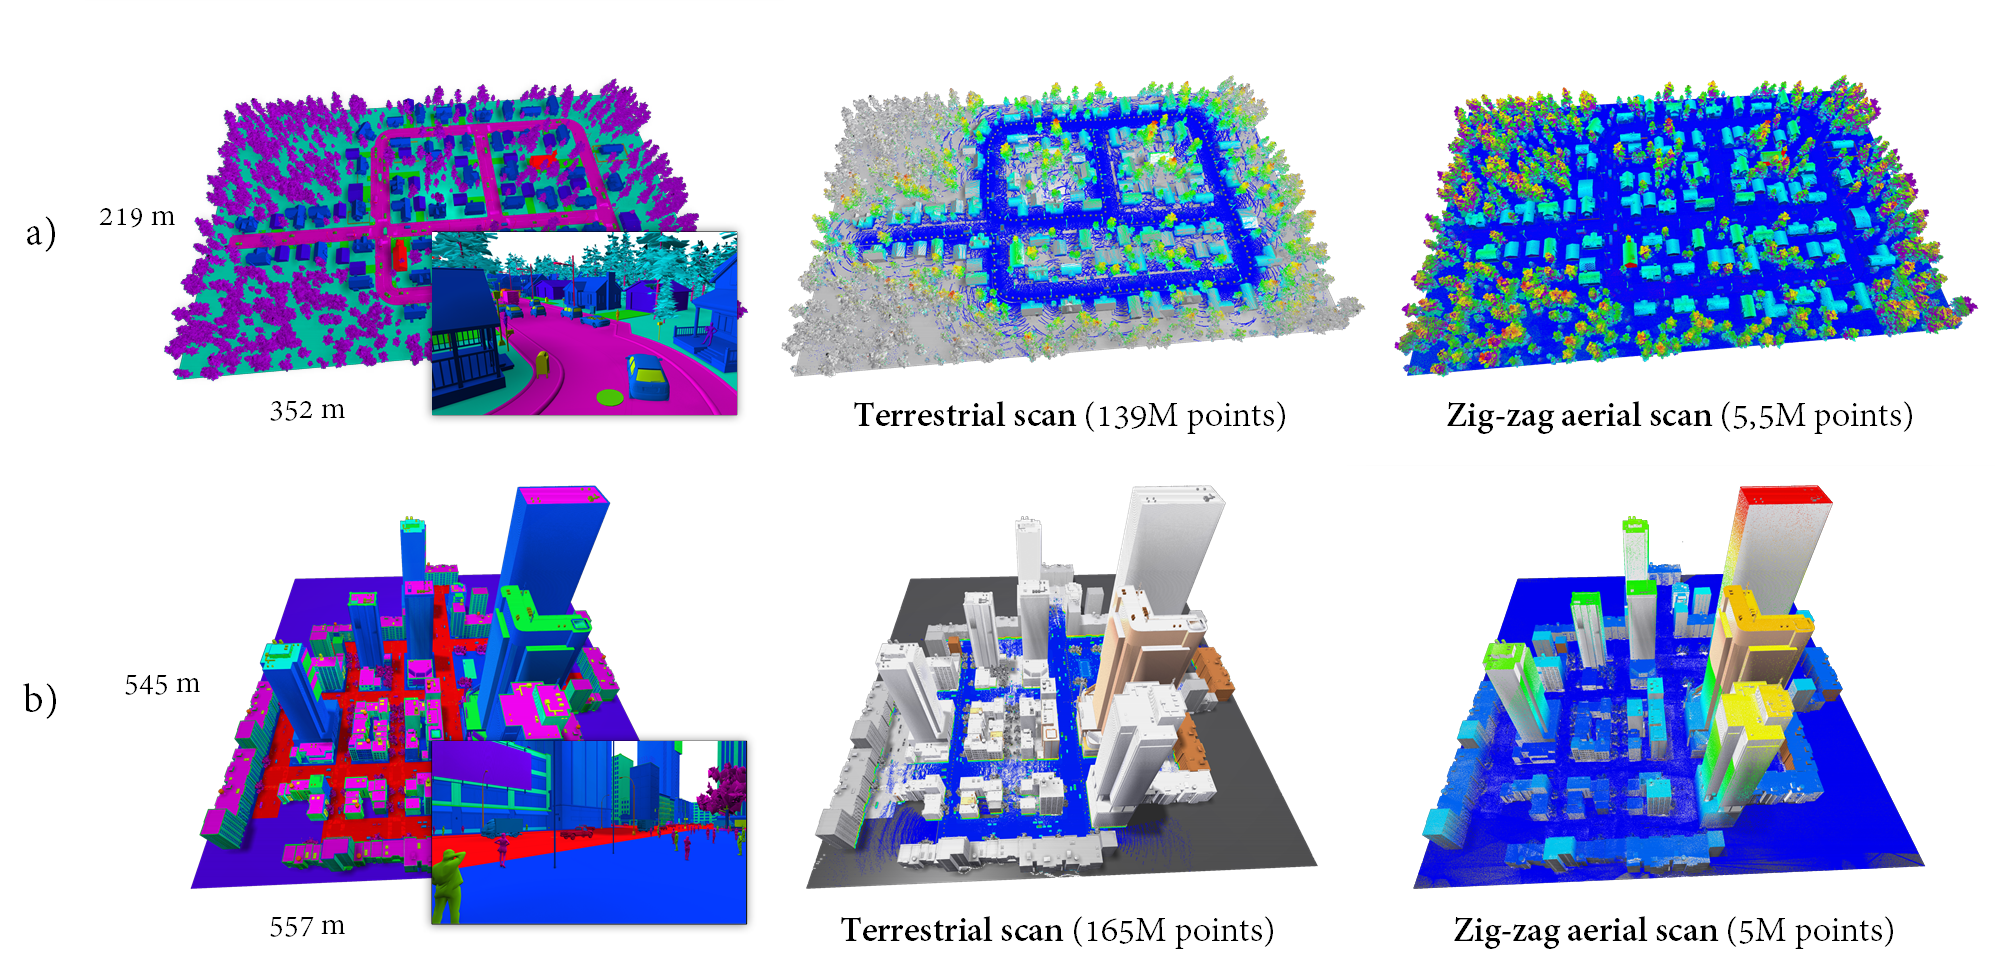
\includegraphics[width=\linewidth]{figs/lidar_simulation/urban_scan.png}
	\caption{Point clouds simulated over urban environments. The input triangle meshes are first depicted, and then, environments are scanned either with \acrshort{tls} or \acrshort{als}.}
	\label{fig:lidar_urban_scan}
\end{figure*}

\renewcommand{\arraystretch}{1.2}
\begin{table*}
    \caption{Specifications of sensors simulated during the scanning of urban environments. Parameters adapted or required by virtual scans are highlighted in cursive.}
    \label{table:test_sensor_parameters}
    \centering
    \begin{tabular}{lcccc}
    \hline
     & \multicolumn{4}{c}{\textbf{Sensors}}\\
    \cmidrule{2-5}
    \textbf{Attributes} & \multicolumn{2}{c}{\textbf{Velodyne HDL-64E} \cite{su_simulation_2019}} & \multicolumn{2}{c}{\textbf{Zenmuse L1} \cite{dji_zenmuse_2020}}\\
    \cmidrule{2-5}
     & Environment 1 & Environment 2 & Environment 1 & Environment 2\\
    \midrule
    Field of view & \multicolumn{2}{c}{360\textdegree $\times$ 26.9\textdegree} & \multicolumn{2}{c}{70.4\textdegree $\times$ 4.5\textdegree}\\
    Resolution & \multicolumn{2}{c}{0.08\textdegree $\times$ 0.4\textdegree} & \multicolumn{2}{c}{~0.1437\textdegree $\times$ 0.00918\textdegree}\\
    Number of channels & \multicolumn{2}{c}{64} & \multicolumn{2}{c}{1}\\
    Vertical \acrshort{fov} origin & \multicolumn{2}{c}{-11.45\textdegree} & \multicolumn{2}{c}{0\textdegree}\\
    Maximum range & \multicolumn{2}{c}{120 \si{\meter}} & \multicolumn{2}{c}{190 \si{\meter}}\\
    Maximum number of returns & \multicolumn{2}{c}{2} & \multicolumn{2}{c}{3}\\
    Scan altitude* ($h_{l}$) & \multicolumn{2}{c}{2 \si{\meter}} & 45 \si{\meter} & 115 \si{\meter} / 290 \si{\meter}\\
    Platform speed* ($s_{p}$) & \multicolumn{2}{c}{--} & \multicolumn{1}{c}{2 \si{\meter}/\si{\second}} & 0.5 \si{\meter}/\si{\second}\\
    Rays within a pulse* ($n_{r}$) & \multicolumn{2}{c}{5} & \multicolumn{2}{c}{5}\\
    \midrule
    Pulses per scan* & \multicolumn{2}{c}{302,625} & \multicolumn{2}{c}{240,000}\\
    \midrule
    Generated rays & 342M & 30M & 390M & 72M\\
    Resulting points & 139M & 5.5M & 165M & 5M\\
    \bottomrule
    \end{tabular}\\
    \footnotesize{$^*$ These parameters were not provided by the manufacturer and thus were adjusted with the objective of providing a dense result.}\\
\end{table*}
\renewcommand{\arraystretch}{1}

\subsection{Visual results}

Besides quantitative tests, comparisons were also established by means of visual results using real-world \acrshort{lidar} point clouds as the baseline result. Furthermore, these tests were carried out over \acrshort{cad} models instead of polygonal meshes extracted from previous scans, as the latter introduces geometrical errors. Vehicles were selected as the target since their \acrshort{cad} models were easier to collect and they are also very frequently scanned in publicly available \acrshort{tls} urban datasets. The compared dataset was obtained from a Pandar64 sensor \cite{hesai_pandaset_2021} that provided \acrshort{rgb} images and individual \acrshort{tls} scans. This way, individual scans were compared instead of point clouds obtained from several viewpoints. 

Regarding other virtual simulators, most of the revised work provides datasets rather than the simulator itself, operates only in pre-defined environments \cite{lg_electronics_rd_lab_lgsvl_2021}, or does not integrate surface materials \cite{yue_lidar_2018, xiao_synlidar_2021, manivasagam_lidarsim_2020, fang_augmented_2020, su_simulation_2019}. Others lack non-uniform scanning \cite{dosovitskiy_carla_2017} and noise/loss behaviour \cite{shah_airsim_2017}. Consequently, comparisons have been performed against the widespread blender plugin Blensor \cite{gschwandtner_blensor_2011}: it is an open-source project that also implements a naïve simulation of noise and errors derived from reflective surfaces. The scenario was configured so that some car materials were modelled as highly reflective (e.g., glasses), whereas the \acrshort{lidar} location was configured according to the real \acrshort{lidar} placement. In addition, the Pandar64 \acrshort{lidar} presents different spatial resolutions along the vertical axis. In contrast to previous work, the proposed solution also supports this kind of sensor. Finally, a loss function was defined for glossy surfaces, over which reflection errors were emulated. Nevertheless, note that the effects derived from 'time-walk' are harder to notice due to the reduced distance between the sensor and the target surfaces. 

Figure \ref{fig:lidar_point_cloud_comparison} shows that glossy surfaces are omitted by Blensor, whereas the point clouds obtained from our simulator have some gaps as a result of the loss function. On the other hand, Blensor includes a noise function defined by its amplitude and distribution to include some variability in the final point cloud. Consequently, both virtual \acrshort{lidar} sensors generate results following patterns similar to the real \acrshort{lidar}, including noisy point clouds; however, reflection errors were better emulated by the proposed solution in a lower response time.

\begin{figure*}
    \centering
    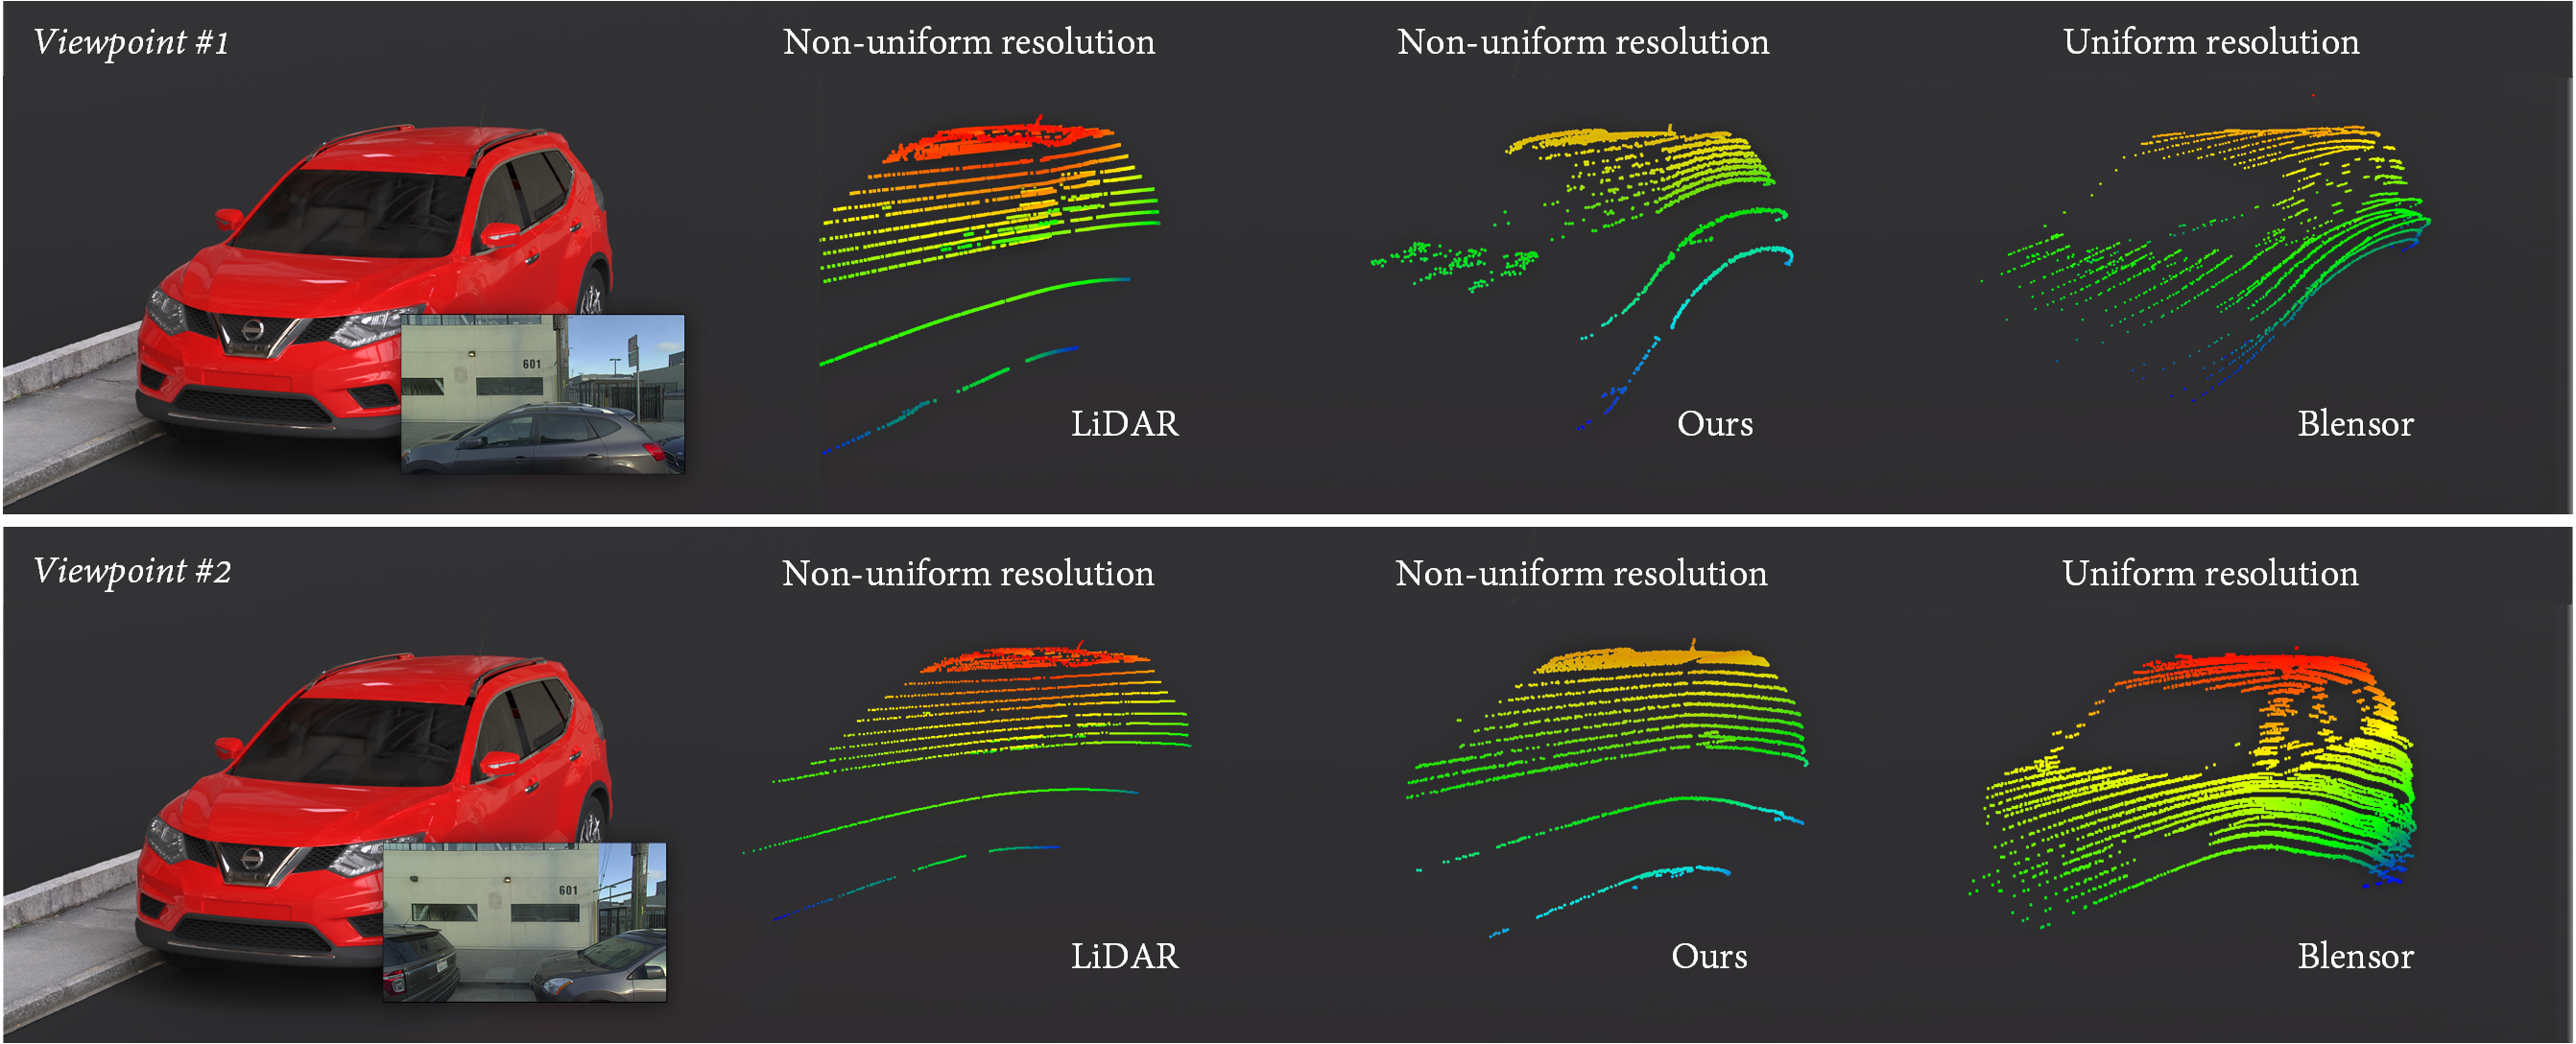
\includegraphics[width=\linewidth]{figs/lidar_simulation/lidar_point_cloud_comparison.png}
	\caption{Comparison of real and synthetic point clouds. The first two images depict the input \acrshort{cad} model and its corresponding \acrshort{lidar} point cloud as captured from a Pandar64 sensor \cite{hesai_pandaset_2021}. The third image illustrates a synthetic point cloud from our simulator, and finally, the fourth image shows the result from the Blensor plugin with a uniform vertical resolution. }
	\label{fig:lidar_point_cloud_comparison}
\end{figure*}

\section{Conclusions and future work}

A massively parallel and parameterized \acrshort{lidar} was proposed for generating dense semantic point clouds, aimed at collecting large datasets for \acrshort{dl} models. It operates over any environment defined as a triangle mesh. However, procedural scenes were constructed to provide a time-efficient alternative that alleviates the manual annotation task. Procedural environments are labelled once and produce large datasets, whereas static environments only contribute to building a few point clouds at most. Spatial queries were rapidly solved with state-of-the-art data structures proposed for ray tracing, whereas the proposed \acrshort{tof} solver includes multiple returns and well-known \acrshort{lidar} errors. To this end, \acrshort{lidar}'s pulses were discretized as several rays that strike into the scene surfaces, instead of solving the simulation in the image space. Thus, the described algorithm is suitable both for real-time simulations and the generation of large \acrshort{lidar} semantic point clouds with low latency. Accordingly, \acrshort{lidar} scans can be solved iteratively or in a single batch. Also, the sensor parameterization helps in simulating a wide range of \acrshort{lidar} sensors and platforms, including \acrshort{als}.

This solution was assessed through its performance and capabilities in the generation of large datasets. The workflow was implemented in \acrshort{glsl} and compared with its analogous multi-core \acrshort{cpu} approach by conducting much more dense scans than actual \acrshort{lidar} sensors. These tests showed that the \acrshort{gpu} approach improves the sequential procedure with speedups above 90\%. Hence, it was also demonstrated that this simulator is appropriate for generating large semantic \acrshort{lidar} datasets with low latency, despite working with large and highly detailed scenes. Regarding scanning capabilities, a significant enhancement both in average scan size and the number of semantic labels was observed. Note that this is not solely affected by the \acrshort{lidar} scans, but also as a result of the facilities given on the annotation task. Finally, point clouds were visually compared against the results obtained using the Blensor plugin, proving that some errors, such as those derived from highly reflective surfaces, were better simulated by our solution. 

In future work, the proposed pipeline could be further accelerated in multi-\acrshort{gpu} systems. Furthermore, this framework could be extended to cover full-waveform and single-photon \acrshort{lidar} \cite{tachella_real-time_2019} and other nonincluded systems. Finally, a deeper study ought to be conducted to show the benefits of synthetic \acrshort{lidar} point clouds in the training of \acrshort{dl} networks, thus checking whether datasets can be partially or completely exchanged by synthetic data. 